\documentclass{aamas2012}
\usepackage{times}  
\usepackage{helvet}     
\usepackage{courier}  
\usepackage{amsmath}  
\usepackage{multirow}
\usepackage{algorithmic}
\usepackage{algorithm}
\usepackage{amsthm}  
\usepackage{graphicx}   
\usepackage{textcomp}
\usepackage{amssymb}
\usepackage{subfigure}
\usepackage{xcolor}  
\usepackage{url}
\usepackage{tkz-2d}
\usepackage{multirow}
\usepackage{tikz}
\usepackage{tkz-berge}    
\usepackage{enumitem}
\newtheorem{definition}{Definition}
\newtheorem{theorem}{Theorem}
\newtheorem{example}{Example}
\usepackage{listings}
\usepackage[caption=false]{subfig}
\usepackage{array}
\usepackage{tabularx}
\usepackage{subfigure}
\usepackage{url}
\author{
\alignauthor Paper  5
}
\title{Stable coalition formation among energy consumers in the
smart grid}
\begin{document}
\maketitle
\begin{abstract}
The vision of the Smart Grid includes demand-side peak shaving strategies, such
as real-time pricing or profile's based tariffs, to encourage consumption such
that the peaks on demand are flattened. Up to date, most works along this line
focused on optimising via scheduling of home appliances or micro-storage the
individual user consumption. Alternatively, in this paper we propose to exploit
the consumer social side by organising them into coalitions of energy users with
complementary needs. To this ends\ldots
% In this paper we propose a general procedure to compute a core element (or to
% detect that no core allocation exists) which is based on mathematical
% programming techniques.
%
\end{abstract}

\section{Introduction}

Since energy cannot be stored efficiently on a large scale, the electricity grid
must perfectly balance the demand of all customers at any instant with supply.
In all current electricity grids this balance is achieved by varying the
supply-side to continuously match demand. The amount of demand required on a
continuous basis is usually carried by the baseload stations owing to low cost
generation, efficiency and safety. However, these stations are slow to fire up
and cool down, so they are not able to match the peakload periods that exceed
this baseload that require, in contrast, the use of expensive, carbon-intensive,
peaking plants generators. Although only running when there is high demand,
these peaking plants generators are responsible of most part of consumers
electricity bill.

Along this line, the vision of the Smart Grid includes demand-side peak-shaving
strategies such as real-time pricing or profile's based tariffs to encourage
consumption such that the peaks on demand are \emph{flattened} \cite{}. A
flattened demand results in a more efficient grid not only with lower carbon
emissions but also with lower prices for consumers. Hence, some works \cite{}
focused on techniques that flatten individual consumer demand by automatically
controlling home domestic or micro-storage devices. Unluckily, since each
consumer independently optimises its own consumption, the effectiveness of this
approach has a clear limit on the consumer's restrictions and comfort (e.g. it
will be unavoidable to get a consumption peak in the non-working hours of
consumers).

Against this background \ldots


\section{Background}
$p_F$ is the unit energy price in the forward market.
$p_A$ is the unit energy price in the day-ahead market.

\begin{figure}[!bt]
\hspace{-0.2in}\subfigure[$G$]{
	\tikzstyle{node} = [circle,line width = 1pt,text width=1.5em, text centered,color=black,draw]
	\tikzstyle{arrow} = [line width = 1 pt]
	\begin{tikzpicture}[scale=0.6,transform shape]
		\node[node] (0) at (-1,7) {\large$a_0$};
		\node[node]  (1) at (-1.5,5.5) {\large$a_1$};
		\node[node] (2) at (-2,4) {\large$a_2$};
		\node[node] (3) at (-0.5,5.5) {\large$a_3$};
		\node at (0,5) { };
		\path[-]	(1) edge[arrow,sloped, above] node {} (2)
					(0) edge[arrow,sloped, above] node {} (1)
					(0) edge[arrow,sloped, above] node {} (3)
					(0) edge[arrow,bend right, above] node {} (2);
			\end{tikzpicture}

} 
\hspace{-0.2in}\subfigure[$PT$]{
	\tikzstyle{node} = [circle,line width = 1pt,text width=1.5em, text centered,color=black,draw]
	\tikzstyle{arrow} = [line width = 1 pt]
	\begin{tikzpicture}[scale=0.6,transform shape]
		\node[node] (0) at (-1,3) {\large$a_0$};
		\node[node]  (1) at (-1.5,1.5) {\large$a_1$};
		\node[node] (2) at (-2,0) {\large$a_2$};
		\node[node] (3) at (-0.5,1.5) {\large$a_3$};
		\node at (0,5) { };
		\path[<-]	(1) edge[arrow,sloped, above] node {} (2)
					(0) edge[arrow,sloped, above] node {} (1)
					(0) edge[arrow,sloped, above] node {} (3);
		\path[-]	(0) edge[arrow,dashed, bend right, above] node {} (2);
	\end{tikzpicture}
}  
% \subfigure[Characteristic function]{
% 	\tikzstyle{node} = [circle,line width = 1pt,text width=1.5em, text centered,color=black,draw]
% 	\tikzstyle{arrow} = [line width = 1 pt]
% 	\begin{tikzpicture}[scale=0.6,transform shape]
% 		\node at (4,5.5) {
% 		\large
% 		\begin{tabular}{ | c |  c |  c | }
% 			\hline
% 			\multirow{2}{*}{$\mathcal{F}(G)$} & \multicolumn{2}{|c|}{$v(\cdot)$}\\
% 			\cline{2-3}
% 			 &    &  \\
% 			\hline
% 			\{0\} &  &  \\
% 			\{0,1\} &  & \\
% 			\{0,1,2\} &  &  \\
% 			\{0,2\} & &  \\
% 			\{0,3\} & & \\
% 			\{0,1,3\} &  &  \\
% 			\{0,2,3\} & &  \\
% 			\{0,1,2,3\} &  &  \\
%   			\{1,2\} &  &  \\
%   			\{1\} &  & \\
%   			\{2\} &  & \\
%   			\{3\} &  & \\
%   			\hline
%   			\multicolumn{1}{c}{ } & \multicolumn{1}{c}{} &\multicolumn{1}{c}{}\\
%   			\hline
%   			\multicolumn{1}{|c |}{$CS^*$} & \multicolumn{1}{|c|}{$\{\{0,2\},\{1\}\}$} &
%   			\multicolumn{1}{|c|}{$\{\{0,1,2\}\}$}\\
%   			\hline
%   			\multicolumn{1}{|c|}{$\rho$}
%   			& \multicolumn{1}{|c|}{$\{1.1, 0.6, 0.9\}$}&
%   			\multicolumn{1}{|c|}{$\emptyset$}\\
%   			\hline
%   			%\multicolumn{3}{c}{$ \{0,1,2\}$}\\
% 		\end{tabular}
% 		};
% 	\end{tikzpicture}
% }  
\caption{\label{fig:cycle_graph} Example of (a) a graph with a
cycle ($G$); (b) a pseudotree $PT$ of $G$; and (c) a clique tree of $PT$.}
\end{figure}  
\subsection{Today's electricity market}
 
In most European countries, the current operation of the exchange electricity
market is composed of multiples markets available for trading electricity,
each with different operation and purpose \cite{vademecumitaly, marketrules} .
In particular, most countries define and distinguishes, at least,
between two kinds of markets: the \emph{spot electricity markets} and the
\emph{forward electricity markets}.
The main goal of spot markets lies in the facilitation of the
trading of short-term energy delivery. In a spot market energy is traded
independently for each time slot and hence, each time slot may have a different
price (e.g.
the day-ahead market is a spot market where hourly blocks of electricity are negotiated
for the next day).
In contrast, forward markets is the venue where forward
electricity contracts for long periods (e.g. month, quarter or year) with
delivery and withdrawal obligation are negotiated.
Thus, the contract in a forward market specifies a single quantity that
will be delivered at constant rate for the contract period and a single
price.

Up to date, even most countries in the EU are now liberalised, market
operation restricts explicitly or implicitly the participation to
wholesale companies that subsequently will offer electricity to final consumers
in form of standard products.
However, in the smart grid .
As part of the smart grid community, electricity consumers have already access
to smart meters that allow them to monitor its (load) energy profile in an
hour-day basis. Thus, the energy profile of a consumer $a_i$ can be represented
as a vector $E_i=\{e^1_i,\ldots,e^N_i\}$ where $e^t_i$ is the amount of energy
consumed at time slot $t$.
Figure shows an example of energy profile as a graph that plots the variation
in the electrical load versus time.
  
in time units.
The most typical type unit is the hour.
 
MWh. 



For electricity, the unit of measurement is the MWh.





\subsection{Coalitional games}

A coalitional (''transferable utility'' or ''characteristic function'') game is
traditionally defined as follows. Let $A=\{a_1,\ldots,a_n\}$ be a set of agents.
A subset $S\subseteq A$ is termed a coalition. However, depending on the domain
not all coalitions may be feasible. In particular, here we are interested on
restricting coalitions by a \emph{graph} $G$: (i) each node of the graph
represents an agent; and (ii) a coalition $S$ is allowed to form iff every two
agents in $S$ are connected by some path in the subgraph induced by $S$. We
denote the set of graph feasible coalitions as $F(G)$.
Then, a coalitional game $CG$ is completely defined by its {\em
characteristic function}  $v: F(G) \rightarrow \Re$, which assigns a real value representing
(transferable) utility to every feasible coalition~\cite{osborne}.
Agents in a coalition are then permitted to freely distribute coalitional
utility among themselves. Given a game $CG$, a {\em coalition structure} $CS=
\{S_1, \ldots, S_k\}$ is an exhaustive disjoint partition of the space of agents
into feasible coalitions. We overload notation by denoting by $v(CS)$ the
(intuitive) worth of a coalition structure: $v(CS) = \sum_{S \in CS} v(S)$. 
%We also denote
%the set of all coalition structures by $\mathbf{CS}$.


Then, the coalition formation process can generally be considered to include
three differentiated activities: \emph{Coalitional Value Calculation},
\emph{Coalition Structure Generation} and \emph{Payoff Distribution}.
First, on \emph{coalitional value calculation}, agents enumerate and evaluate
all possible feasible coalitions that can be formed. 
Next, given the values of feasible coalitions, the key challenge addressed in
\emph{coalition structure generation} is to identify the coalition
structure $CS^*$ that maximizes \emph{social welfare} - i.e. the coalition structure with
maximal value.
%\begin{equation}
%CS^* = arg \max_{CS\in \mathbf{CS}} v(CS)
%\end{equation}
%The CSG problem is NP-hard~\cite{DBLP:journals/ai/SandholmLAST99}.
Finally, \emph{Payoff Distribution} determines the utility that each agent in a
coalition should obtain as a result of the actions taken by the coalition as a
whole. A vector $\rho = \{\rho_1, \ldots, \rho_n\}$ assigning some payoff to each agent
$a_i \in A$ is called an \emph{allocation}.
We denote $\sum_{i\in S}\rho_i$ by $\rho(S)$.
An allocation $\rho$ is an {\em imputation} for a given $CS$, if it is
efficient ($\rho(S) =v(S)$ for all $S \in CS$), and individually rational (that
is, $\rho_i \geq v(\{i\})$ for all $a_i$). Note that if $\rho$ is an imputation
for $CS$, then $\rho(A) = v(CS)$.
A game outcome is a $(CS,\rho)$ pair, assigning agents to
coalitions and allocating payoffs to agents efficiently. However, in a selfish
environments, agents are only concerned with maximizing their own payoffs.
Thus, with the presence of selfish
agents we need to the determine \emph{stable} allocations.
Here, stability refers to
the state where the agents have no incentive to deviate from the coalitions to
which they belong. Cooperative game theory provides several stability concepts
and one concept, the core which is arguably the most well-studied shall be
discussed here. The core is composed of all coalition structure-imputation
tuples $(CS, \rho)$ such that no feasible coalition has a deviation incentive.
Formally:


\small
\begin{equation}
\hspace{-0.05in}Core(CG) = \{ (CS,\rho): \rho(A) = v(CS) \ \& \ \rho(S) \geq
v(S) \ \forall S \in F(G) \} \notag
\end{equation}
\normalsize

\noindent The core is a strong solution concept, as it is
empty in a plethora of games. Moreover, notice that \emph{only optimal coalition
structures might admit an element in the core}. Intuitively, if the current structure is suboptimal then a
subset of agents can be made strictly better off by moving to an optimal
coalition structure. Hence, for any core-pair allocation $CS$ is an optimal
coalition structure, $CS^*$, and the allocation $\rho$ is efficient with respect of the value of the optimal coalition structure ($\rho(A) = v(CS ^*)$).
In this work, we are interested on the question of how to compute a core member:
this includes to solve the CSG problem to get the optimal coalition structure
$CS^*$ and compute the stable payoff allocation over $CS^*$ or
detect the emptiness of the core if it is the case.


%Therefore, the question of the core non-emptiness is a key in many settings.
%However, this does not mean that a game outcome is necessarily stable; there
% might be agents that feel there are outcomes that can make them better-off.
%Unlike cooperative environments, where the agents are mainly concerned
%with maximizing the social welfare, the agents in a selfish environment are
% only concerned with maximizing their own utility. Thus, with the presence of selfish
%agents we need to the determine stable allocations. Here, stability refers to
%the state where the agents have no incentive to deviate from the coalitions to
%which they belong.

\section{The model}
\label{sec:the_model}
In this section, we model the problem of demand-side coalition formation among
energy consumers as a coalitional game. Let $A=\{a_1,\ldots,a_n\}$ be the set of
agents, each one representing an energy consumer with its associated energy
profile $E_i$.
Agents can form energy coalitions $S\subseteq A$, where an energy coalition $S$ stands for the set of
consumers $S$ acting as a single virtual consumer in the market along with
their joint consumption. Analogously to single consumer coalitions, the
(expected) demand of any coalition of consumers $S$ is represented by their
joint energy profile $E_S=\{e^1_S, \ldots, e^N_S\}$ where $e^t_S=\sum_{i\in S}
e^t_i$. By forming coalitions, agents can join other consumers with
complementary energy needs, getting a flattened demand for which they can get better prices in the market. 
Hence, regarding the coalitional value calculation, the value of a
coalition among energy customers $v(S)$ needs to codify the expected payment
that the coalition of consumers $S$ will need to carry out to get their joint demand.  Moreover, we consider that each consumer looks for potential partners
for its coalitions through its contacts in a social network. 
 Thus, the set of energy feasible
coalitions is constrained by a graph $G$.

In the next sections, we specify with more detail how we solve the three main
activities that underline the coalition formation process for this particular
energy domain.


\subsection{Coalitional Value Calculation}
To capture such complementarities, in
Section we define the characteristic function $v(\cdot)$ for this domain, where $v(S)$ stands for the expected payment that the coalition of consumers $S$ will need to carry out to get their joint demand.
We address the problem of enumerating and evaluating all energy coalitions in
the social network in Section .
\subsubsection{Characteristic function definition}
To capture such complementarities, in
Section we define the characteristic function $v(\cdot)$ for this domain, where $v(S)$ stands for the expected payment that the coalition of consumers $S$ will need to carry out to get their joint demand.

The value of a coalition S, $v(S)$, is the total payment that the set of
consumers need to carry out to cover the demand of their joint energy profile. 
Analogously to the operation of the current grid, we consider that consumers buy
directly their electricity in two different markets: the Spot Electricity
Market and the Forward Electricity Market. 
We use the joint average energy profile of a coalition as a prediction of its consumption. Then one question that emerge is how members of a
coalition can buy their excepted consumption in the available markets (spot and
forward market) in order to minimize the amount to be paid. We denote
$p_{Spot}$ and $p_{Forward}$ to the prices of the spot and the forward market
respectively. Explain that the price of the spot is the average among hours and
the price of the forward is the price for one hour. Agents in a coalition need
to decide the quantity they buy in the forward market $q^{F}$ and the quantity
they buy on the spot market $q^i_{Spot}$ for each time slot 1\ldots N. Agents
need to decide these quantities such that the demand for each time slot is
covered. Formally,
\begin{equation}
e^i \geq q^i_{Spot} + q_{Forward} \ \ \forall i= 1\ldots N
\label{eq:covered}
\end{equation}


 Then, the value of the expected
payment for the coalition $S$ is given by:
\begin{equation}
v(S) = -( \sum^N_{i=1}q^i_{Spot} \cdot p_{Spot} + q_{Forward}\cdot N \cdot
p_{Forward} )
\label{eq:objective}
\end{equation}

Agents need to decide the continuous amount of quantity they buy in the forward
market $q_{Forward}$ as well as the quantity they buy in the spot market for
each time slot i such that maximise equation \ref{eq:objective} whereas
satisfying constraints in equation \ref{eq:covered}.



 In the forward market, consumers in a coalition
$S$ buy in advance the fix continuous amount of energy of their joint energy profile,
$base(S)$, for a better price. To compute the base load from an energy profile
you simply compute the minimum of the energy consumption along hours and
$base(S) = min*24 h$. $peak(S)= sum_{h} - base(S)$.

The amount of energy that exceeds this baseload,
$peak(S)$, is bought in the day-ahead market.
\begin{equation}
v(S) = -base(S) \cdot p_F - peak(S) \cdot p_A
\end{equation}

Since $p_F<p_A$, the flattered the energy profile, the most a coalition of
consumers can buy in the forward market and the lower the payment of the
coalition.

Another measure?



\subsection{Network-based coalitions}

% \begin{algorithm}[!tb]
% \caption{\textbf{generateCoalitionsOnAGraph}\label{proc:generateCoalitionOnAGraph}}
% Each agent runs:
% \begin{algorithmic}
% \STATE $converged \leftarrow false;$
% \STATE $Req_i \leftarrow \emptyset;$
% \STATE $rn_i \leftarrow getReqNumber();$
% \STATE requestCoalitionsMessages($rn_i$,$rn_i$,
% $a_i$,$a_i$,$\langle \emptyset,\emptyset, null \rangle$);
% \WHILE{! global\_convergence}
% \STATE Wait for any incoming $msg$ message. Let $a_k$ be the sender.
% \IF{$msg$ is a $ReqCoalitions(rn_l, a_l, \langle S, E, a_h \rangle)$
% message }
% \STATE $rn \leftarrow getReqNumber();$
% \STATE sendRequestCoalitionsMessages($rn$,$rn_k$,
% $a_l$,$a_k$,$\langle S, E, a_h \rangle$);
% \ELSIF{$msg$ is a $Coalitions(rn, \mathbf{S})$}
% \STATE $info(rn).\mathbf{S}(a_k)\leftarrow \mathbf{S} $/*Store
% coalitions*/ 
% \STATE $info(rn).R \leftarrow info(rn).R
% \cup \{a_k\};$
% \IF{$info(rn).Q == info(rn).R$ /*All agents sent
% coalitions*/} \STATE cross-over(rn);/*Do the cross-over*/
% \IF{$rn == rn_i$}
% 	\STATE $converged \leftarrow true;$
% \ELSE
% 	\STATE Send
% 	$Coalitions(info(rn).rn_s,info(rn).\mathbf{S})$
% 	to $info(rn).a_s$;
% \ENDIF
% \ENDIF
% \ENDIF
% \ENDWHILE
% \FORALL{$required(S)$ msg received}
% 	\STATE Let $a_k$ be the sender agent
% 	\IF{$Req_i(S \setminus \{a_k\}) == \emptyset$}
% 		\STATE $ Req_i(S) \leftarrow S \setminus \{a_k\}; $
% 	\ELSE
% 		\STATE $ Req_i(S) \leftarrow Req_i(S \setminus \{a_k\});$
% 	\ENDIF
% \ENDFOR
% \RETURN $info(rn_i).\mathbf{S}$
% \end{algorithmic}
% \end{algorithm}
% 
% \begin{algorithm}[!tb]
% \caption{\textbf{cross\_over(rn)}}
% \begin{algorithmic}
% \IF{$rn == rn_i$/*Crossing over local coalitions*/}
% 	\FORALL{$a_j\in info(rn).Q, \langle S, E,a_h\rangle
% 	\in info(rn).\mathbf{S}(a_j)$}
% 		\STATE $Req_i(S) \leftarrow \emptyset;$
% 		\STATE Send $required(S)$ to $a_h$;
% 	\ENDFOR
% \ENDIF
% \FORALL{$a_j\in info(rn).Q$}
% \STATE $info(rn).R \leftarrow info(rn).R
% \setminus \{a_j\};$
% \FORALL{$a_k\in info(rn).R $}
% 		\STATE /*Do the cross-over between coalitions received from $a_j$ and
% 		coalitions received from $a_k$*/
% 		\FORALL{$\langle S, E,a_h\rangle \in
% 		info(rn).\mathbf{S}(a_j)$}
% 		\STATE $\mathbf{S}_{new} \leftarrow \emptyset;$
% 		\FORALL{$\langle S', E',a'_h\rangle \in
% 		info(rn).\mathbf{S}(a_k)$}
% 		\IF{$E\cap S' == info(rn).\mathbf{S}(a_j).S$}
% 			\IF{$rn == rn_i$/*Crossing over local coalitions*/}
% 				\IF{$Req_i(S)==\emptyset$}
% 					\STATE $Req_i(S\cup S')\leftarrow \{S',S\};$
% 				\ELSE
% 					\STATE $Req_i(S\cup S')\leftarrow \{S',Req_i(S)\};$
% 			 	\ENDIF
% 			 	\STATE $\mathbf{S}_{new} \leftarrow \mathbf{S}_{new} \cup \langle S\cup S',
% 			E\cup E', null\rangle$;/*All the requiring coalitions are in this agent*/
% 			\ELSE
% 				\STATE $\mathbf{S}_{new} \leftarrow \mathbf{S}_{new} \cup \langle S\cup S',
% 			E\cup E', minlevel(a_h,a'_h)\rangle$;
% 			\ENDIF
% 		\ENDIF
% 		\ENDFOR
% 		\STATE $info(rn).\mathbf{S}(a_j).\langle S, E, a_h\rangle \leftarrow \langle
% 		S, E \cup \{a_j\}, a_h\rangle;$ \STATE $info(rn).\mathbf{S}(a_j)\leftarrow
% 		info(rn).\mathbf{S}(a_j) \cup \mathbf{S}_{new};$
% 		\ENDFOR
% \ENDFOR
% \ENDFOR
% \end{algorithmic}
% \end{algorithm}


%  \begin{algorithm}[!tb]
% \caption{\textbf{Procedure
% sendRequestCoalitionsMessages($rn$,$rn_s$, $a_l$,$a_s$, $\langle S, E, a_h
% \rangle$)}}
% \begin{algorithmic}
% \STATE $S\leftarrow S�\cup \{a_i\};$ /*Add
% $a_i$ to the coalition*/
% \STATE $F_i \leftarrow \{ a_j \in N(a_i) \vert a_j.level > a_l.level
% \mbox{ and } a_j \not\in E \}$; /*Get all $a_i$'s neighbours not excluded and with higher
% level than $a_l$ in the DFS*/
% \IF{$a_i \neq a_l $ and $a_i.level < a_h$}
% \STATE $a_h \leftarrow a_i;$
% \ENDIF
% \IF{$F_i == \emptyset$ /*No frontier agent connected to $a_i$*/}
% 	\STATE Send $Coalitions(rn, \{\langle S, E, a_h\rangle\})$ to $a_s$;
% \ELSE
% 	\FORALL{$a_j \in F_i$}
% 		\STATE $E \leftarrow E \cup \{a_j\};$ /*Add $a_j$ to excluded*/
% 		\STATE Send $ReqCoalitions(rn,a_l,\langle S,E, a_h \rangle)$ to $a_j$;
% 	\ENDFOR
% 	\STATE /*Store information to Req\_queue*/
%     \STATE $info(rn).a_l \leftarrow a_l;$
%     \STATE $info(rn).a_s \leftarrow a_s;$
%     \STATE $info(rn).rn_s \leftarrow rn_s;$
%     \STATE $info(rn).\mathbf{S}(a_i) \leftarrow \{\langle S,
% E, a_h\rangle \};$
%     \STATE $info(rn).Q \leftarrow F_i;$
% \ENDIF
% \end{algorithmic}
% \end{algorithm}

To generate the set of graph coalitions we observe that generating all feasible
graph-based coalitions is analogous to the problem of generating all connected
induced subgraphs of a connected undirected graph $G$.
Thus, we formulate an algorithm that allows agents to generate the set of
feasible coalitions in a distributed way. Our algorithm is based on a
state-of-the-art algorithm formulated in \cite{Gutin08analgorithm} that
generates all connected induced subgraphs of a given graph (for further details see \cite{Gutin08analgorithm},
section 5).
The complexity of the algorithm is $O(n\cdot c(G))$, where $n$ is the number of
nodes of $G$ and $c(G)$ is the number of connected induced subgraphs of $G$.
Similarly to Theorem ?, one can prove the following:
(Theorem 10) Let $c(G)$ be the number of connected induced subgraph of a
connected graph $G$. Algorithm is correct and its time and space complexities
are O(n\cdot c(G)) and O(n+m), respectively.
Instead of using a linear ordering as in \cite{Gutin08analgorithm},
we propose to use the partial ordering that defines a pseudotree arrangement
of the agent's graph \cite{}.
Pseudotrees are a common structure used in search and inference procedures
given their ability to exploit independencies between nodes in a graph, allowing
parallel processing of independent branches.

Figure \ref{fig:cycle_graph}(b) shows a pseudotree, rooted at agent
$a_0$, of the cyclic graph $G$ in Figure \ref{fig:cycle_graph}(a). A PT has two kinds of
edges: tree-edges (bold
lines) that link parent with children (e.g. $a_2$ is child of $a_1$); and
pseudoedges (dashed lines) that link pseudoparents with pseudochildren (e.g.
$a_2$ is pseudochild of $a_0$). Let's denote $A(PT)$ the set of agent' nodes
in $PT$ and $PT_i$ the subtree of $PT$ rooted at $a_i$. Thus, in Figure
\ref{fig:cycle_graph}(b), $PT_1$ is a tree rooted at $a_1$ composed of agents $a_1$, $a_2$. Finally, given an agent $a_i\in
A(PT)$ we will denote as $Ch_i$ its children, $An_i$ its ancestors (the set composed of its parent and its pseudoparents), and $D_i$ its descendants (the set composed
of its children and pseudochildren) in $PT$. Then, in Figure
\ref{fig:cycle_graph}(b), $Ch_2=D_2=\emptyset$ and $An_2=\{a_0,a_1\}$.
Then, given a game on a graph $CG=\langle A(G), v, F(G)\rangle$ and a pseudotree
$PT$ over $G$, the partial ordering that $PT$ defines among agents allows
us to partition the set of feasible coalitions into $\vert A \vert$ disjoint
sets $\{\mathbf{L}_i \vert a_i \in A\}$, one per agent. The set
of (leading) coalitions $\mathbf{L}_i$ contains all the
feasible coalitions in which $a_i$ is the leader in the hierarchy, that
is all coalitions that include agent $a_i$ but no agent up $a_i$ in $PT$,
$\mathbf{L}_i = \{S \in F(G_{A(PT_i)}) \vert i \in S \}$). 

Next, we describe the main steps of a distributed procedure that allow agents to
compute the set of leading coalitions on a graph. Thus, at the end of this
process, each agent will know its set of leading coalitions $\mathbf{L_i}$.

Each agent $a_i$ uses the $PT$ partial ordering
 to order its descendants $D_i =
\{d^1,\ldots,d^m\}$ from higher to lower.
For example, in Figure \ref{fig:cycle_graph}(b), $a_0$ can order its descendants
as $a_1$,$a_2$,$a_3$ (as far as $a_1$ is placed before $a_2$ the order is valid).
Then, $a_i$ will proceed to generate its set of leading coalitions
$\mathbf{L}_i$ into two steps: first, generating a
set of basic coalitions, and second, generating a set of composed coalitions,
that result from combination of basic ones.

\noindent \textbf{Step 1. (Basic coalitions).} In this step,
each agent $a_i$ will generate the set of \emph{basic} coalitions.
For each descendant
$d^{j=1\ldots m}$, $a_i$ generates all coalitions $S$ such that $\{d^j\} \subseteq S \subseteq
A(PT_i) \setminus\{E\}$ where $E= \{d_k \vert k< j\}$ stands for all descendants
placed before $d^j$ in the ordering.
For example, in Figure \ref{fig:cycle_graph}(b), agent $a_0$ will
generate the set of coalitions that include:
(i) $a_1$ and other agents reachable from $a_1$ in $PT_1$ ($\{1\}$,$\{12\}$);
(ii) $a_2$ and other agents reachable from $a_2$ in $PT_1$ excluding $a_1$
($\{2\}$); and (iii) $a_3$ and other agents reachable from $a_3$ in $PT_1$
excluding $a_1$ and $a_2$ ($\{3\}$). 

%To generate these sets of coalitions we use a distributed version of a
% recursive algorithm that generates all connected induced subgraphs of a given graph (for
%further details see \cite{Gutin08analgorithm}, section 5).
%The
%procedure in \cite{Gutin08analgorithm} 
Each agent $a_i$ records for each coalition $S$ a
set of frontiers nodes, $F$, these are nodes that are reachable
from $S$ but not included in $S$.
For example, in Figure \ref{fig:cycle_graph}(b) the set of frontiers for 
$\{1\}$ is $\{2\}$ since $a_2$ is reachable from $a_1$ but not
included.

Finally, $a_i$ stores each generated coalition $S$, adding $a_i$,
($S\cup\{i\}$), as well as $a_i$'s single coalition ($\{i\}$), as part of its
leading coalitions $\mathbf{L}_i$.



\noindent \textbf{Step 2. (Composed coalitions).} In this step, each agent $a_i$
will generate the set of \emph{composed} coalitions.
For each descendant $d^{j= 1 \ldots m}$ $a_i$ will combine all coalitions
reachable from $d^j$ with all compatible coalitions reachable from $d^{j+1}$,
from $d^{j+2}$, \ldots, and until $d^{m}$, storing at each step the new
coalitions as reachable from $d^j$.
Thus, in Figure \ref{fig:cycle_graph}(b), $a_0$ will combine coalitions reached
from $a_1$ with coalitions from $a_2$ (storing any new coalition as reachable
from $a_1$) and coalitions reachable from $a_1$ with coalitions from $a_3$.
Two coalitions, $S$ reachable from $d^j$, and $S'$ reachable from $d^{k>j}$, are
compatible if $S'$ does not contain any agent in $S$ or in its frontiers $(S'
\cap S \cap F_S \neq \emptyset)$.  Thus, in Figure \ref{fig:cycle_graph}(b),
$a_1$ will not combine $\{1 \}$ from $a_1$ and $\{2\}$ from $a_2$ because $a_2$
is a frontier for $\{1\}$.
A composed coalition is generated as $\{S\cup S'\}$ with frontier agents
 $\{F_S\cup F_{S'}\}$.
Thus, in Figure \ref{fig:cycle_graph}(b), $a_0$ the result of combining $\{2\}$
from $a_2$ with $\{3\} $ from $a_3$ is a composed coalition $\{2,3\}$ reachable
from $a_2$ with $F=\{2\}\cup\emptyset$.
For each composed coalition resulting from the combination of $S$ with $S'$,
$a_i$ computes its set of requiring coalitions $Req_i(S\cup S'\cup\{i\})$ as
$\{S,S'\}$ if $S$ is a basic coalition or, alternatively, as $\{Req_i(S),S'\}$
if $S$ is a composed coalition.
% In this step, each agent $a_i$
%computes the set of required variables for each composed coalition generated in
% step 2.1. The set of required coalitions for a composed coalition resulting from the combination of $S$ with $S'$, $Req_i(S\cup
%S'\cup\{i\})$, is composed of $\{S,S'$ 
%if $S$ is a basic coalition or, alternatively, of $\{Req_i(S),S'\}$ if $S$ is a
%composed coalition.

% Finally, notice that the set of
%required coalitions for a combined coalition for agent $a_i$ are a set of local
%basic coalitions of $a_i$. Concretely, the required coalitions for a combined
%coalition local to $a_i$ resulting from the combination of $S$ with $S'$,
%$Req_i(S\cup S'\cup\{i\})$ , is composed of: $S$ and $S'$ if $S$ is a basic
%coalition or $\{Req_i(S),S'\}$ if $S$ is a composed coalition. 

%Finally, for each requiring messages received , agent
%$a_i$ adds the requirement to its local requirement function $Req_i(S\cup{j}) =
%\{S\}$ and coalition $S\cup{j}$ to its set of requiring coalitions
%$\mathbf{R}_i$.
%To generate these sets of coalitions we use a distributed version of a
% recursive algorithm that generates all connected induced subgraphs of a given graph (for
%further details see \cite{Gutin08analgorithm}, section 5).
 Explain the way we generate
coalitions.
There is a way to count them?
\cite{Gutin08analgorithm}


\subsection{Coalition Structure Generation}

We now show how to map the CSG defined above into integer programming (IP).
Our aim is to find \ldots.
We define a set of binary decision variables $x_S\in \{0,1\}$, one per feasible
coalition $S\in F(G)$, where $x_S$ takes on value 1 if coalition $S$ is selected and 0
otherwise. Now solving the CSG for the demand-side  amounts to solving the
following IP:

\begin{equation}
max \ \  \sum_{S\in F(G)} v(S) \cdot x_S \notag
\end{equation}

\noindent Subject to:\\


\noindent (1) Each energy customer can join at most one coalition:
\begin{equation}
\forall a_i
\in A: \  \sum_{S \in  F(G) \vert S\ni i } x_S =1 �\notag
\end{equation}

\subsection{Payoff Distribution}
We now show how to map the Payoff Distribution defined above into a linear
program (LP). Following the lemma, x is not blocked if it is not blocked by any
B specified in W. The core is not empty if we can find such a payment vector.
Therefore, the problem that needs to be solved is:

In this paper we propose a general procedure to compute a core element (or to
detect that no core allocation exists) which is based on mathematical
programming techniques.

 Our aim is to find \ldots.
We define a set of binary decision variables $x_S\in \{0,1\}$, one per feasible
coalition $S\in F(G)$, where $x_S$ takes on value 1 if coalition $S$ is selected and 0
otherwise. Now solving the $CSG$ for the demand-side  amounts to solving the
following integer program:
Find stable payments once $CS^*$ has been found by
solving the following LP:\\

\begin{equation}
min \ \ \rho(A) \notag
\end{equation}

\noindent Subject to:\\

\noindent (1) There are no deviating coalitions for these payments:
\begin{equation}
\forall S\in F(G): \  \rho(S) \geq v(S) �\notag
\end{equation}

\noindent (2) Agents can could make a profit
%Agents never get a surplus from the system:
\begin{equation}
\forall a_i\in A : \  \rho_i \leq 0 �\notag
\end{equation}

If the value of the objective function of this IP yields $\rho(A) =v(CS^*)$,
then the problem has a non-empty core and the values $\rho$ define an allocation
in the core. Otherwise, the problem has an empty core.
It should be emphasized that the values $v(S)$ as well as a optimal coalition
structure $CS^*$ are given parameters which means that this program can not
computed the allocation needs as input the results of solving the Coalitional
and the CSG.

If $ v(CS^*)\neq  \rho(A)$ the core is empty. Otherwise the payments
are in the core.
Notice that (2) ensures that agents do not make a profit expoiling from other
agents, getting a positive payoff from payments from other agents in the
coalition. So, as maximum agents can get the energy for free in their best deal.

Linear programs can be solved in polynomial time in the number of variables and
constraints. In our case, the variables are $x_1,\ldots,x_n$ and there are
constraints. The Linear Program will not only specify if the core is not empty,
but also provide $\rho \in CORE$ if one exists.

This program has a number of variables equal to the number of agents
$N_{variables} = \vert A \vert$ and number of constraints equal to the number of
feasible coalitions $N_{constraints} = \vert F(G)�\vert$ which can be very
large (in a complete graph is exponential in $N$).


      
  
\section{Empirical Evaluation}
\label{sec:experiments}
In this section we provide an empirical evaluation of the coalition
formation model among energy consumers introduced in Section
\ref{sec:the_model}. 
Firstly, we explain the details of our experimental setup in Section
\ref{sec:empirical_settings}.
Next, we analyse our empirical results in Section \ref{sec:results}.

\subsection{Empirical settings}
\label{sec:empirical_settings}

\subsubsection{Problem generation}
\label{sec:problem_generation}
To evaluate the sensitivity of the coalition
formation process with respect to the underlying network topology we
evaluate our model on three different network models. Moreover, for each network
topology we analyse networks with different density levels.
The density of a graph is defined as the ratio between the number of links and the number of agents in the graph ($\frac{\vert E \vert}{\vert A \vert}$).
In more detail, in our experiments we test our model on the following network
configurations:
%We compare the results obtained in the coalition formation process among energy
%users on three different network topologies and with three different densities
%that generate low, medium and high density problems:


\vspace{0.1in}\noindent \textbf{Random Networks.} Graphs are created by
\emph{randomly} adding a number of links $d$ for each agent. Densities used in this case are : $d=1$
(low), $d=2$ (medium) and $d=3$ (high).



\vspace{0.1in}\noindent \textbf{Scale Free Networks.} Graphs are created by
using an implementation of the Barabasi-Albert model. At each step, a node is added and
attached to $d$ neighbours using a biased random selection giving more chance to
a node if it has a high degree.
Graphs are generated using three different densities:
($d=0.92$, low), ($d= 1.75$, medium) and ($d=3.17$, high).


\vspace{0.1in}\noindent \textbf{Small-World Networks.} Graphs are created by
following the Watts and Strogatz model.
This model generates a ring of graph where each node is connected to its $k$
nearest neighbours in the ring (k/2 on each side, which means k must be even).
Then it process each node of the ring in order following the ring, and
"rewiring" each of their edges toward the not yet processed nodes with randomly
chosen nodes with a rewiring probability of $0.1$.
Graphs are generated using three different values for parameter k: $k=2$ ($d=1$,
low), $k=4$ ($d=2$, medium) and $k=6$ ($d=3$, high).



Notice that whereas scale free
and small-world networks  are known to capture some characteristics of social
networks, random networks constitute a more synthetic model for our domain.
% Notice that Scale Free
%Networks and Small-World Networks are now to capture some characteristics of
% the real-word social networks whereas and hence, represent more realistic networks for our domain than not Random Networks.
All experiments are run using networks of 12 nodes. For each instance, the
energy profile of each node is randomly selected from a  real dataset composed
of energy profiles characterizing the real domestic electricity consumption
of X homes in the United Kingdom.
% In our experiments we use the average user energy profile
%of consumers in the United Kingdom. 

%Measure of fee of 0. \texteuro/MWh
%The
%day-ahead market price is calculated by averaging the hourly price of 
\subsubsection{Market's parameters}
\label{sec:market_parameters}
As explained in Section , two of the most important parameters that regulate the
electricity market are the prices of the electricity in the forward, $p_{DA}$,
and the day-ahead market, $p_{DA}$ (although the price of electricity in the
day-ahead market varies on each time slot, we consider here that $p_{DA}$ is
calculated by averaging the hourly price of a day).
Moreover, in addition to the market prices, another sensitive parameter is the choice of the strategy to decide which is the
base amount to buy in the forward market (defined through fraction parameter
$p$).
Then, in our experiments, we explore three different market conditions:
\begin{itemize}
  \item[M1] $p_F=70$, $p_{DA}=80$, $p=1$
  \item[M2] $p_F=70$, $p_{DA}=80$, $p=0.875$
  \item[M3] $p_F=1$, $p_{DA}=2$, $p=0.5$
\end{itemize}

Notice that whereas in M1 agents follow a risk-free strategy ($p=1$), in M2 and
M3 agents takes the maximum much risk that gives them a positive expected gain
($p=\frac{p_F}{p_{DA}}$). Regarding market prices, in $M1$ and $M2$ prices used
are those of current electricity markets in Italy\footnote{Available at:
\url{http://www.mercatoelettrico.org/En/Default.aspx} } whereas $M3$ explores a
different scenario in which buying in the forward market is more incentivized
with better prices. As a consequence, the maximum relative
percent gain\footnote{We compute the maximum relative percent gain as the
difference between the cost of buying all demand in the day-ahead market and the cost of buying all demand in the
forward market divided by the cost of buying all demand in the day-ahead
market $100\cdot\frac{p_{DA}-p_{F}}{p_{DA}}$.} an agent can get in M1 and M2
is of $12.5\%$ whereas in M3 is of $50\%$.
 

\subsection{Results}
\label{sec:results}
Using the different configurations explained in section above, we evaluate our
model by performing repeated simulations (50 instances per graph configuration)
and analysing the results in terms of the individual consumer gain and the
structure of the formed coalitions.

%the standard deviation divided by the square root of the
%number of instances.
% \begin{figure*}    
%   \centering  
%   \hspace{-0.1in}\subfigure[Random Graphs.]{
% 	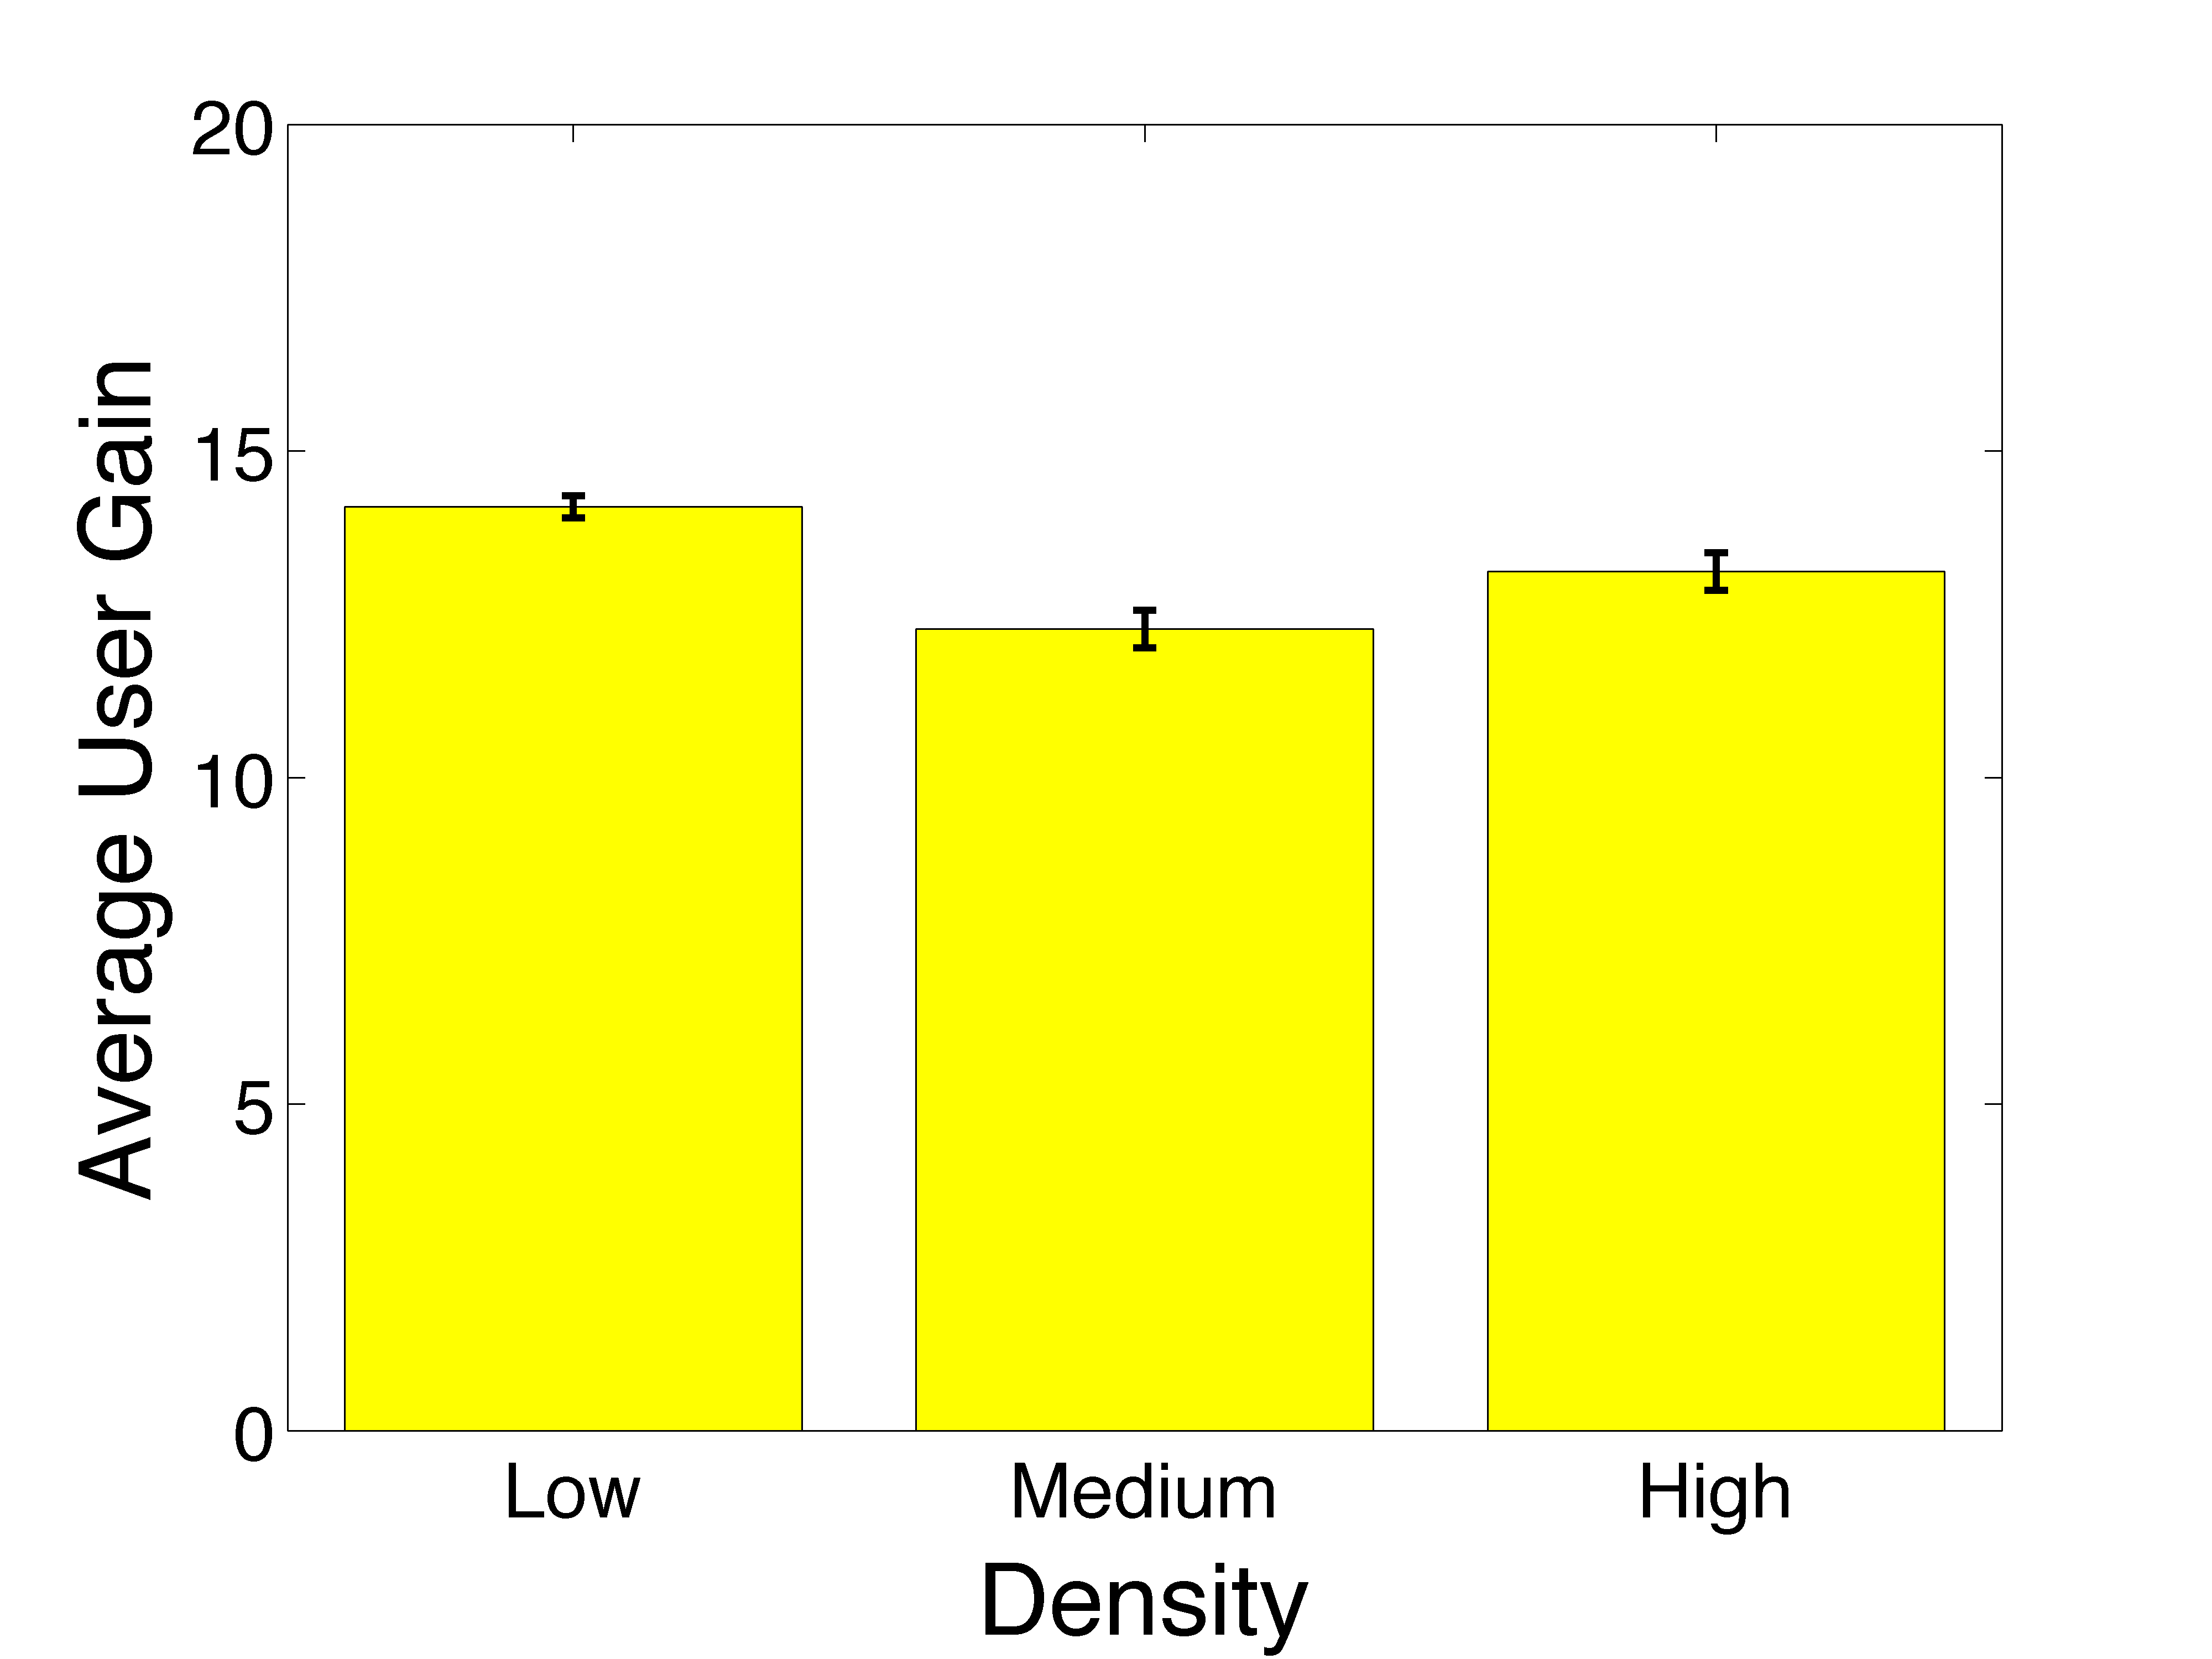
\includegraphics[width=0.33\textwidth,type=png,ext=.png,read=.png]{img/Random-1.000-AUG}
% 	}  
%   \hspace{-0.1in}\subfigure[Scale Free.]{
% 	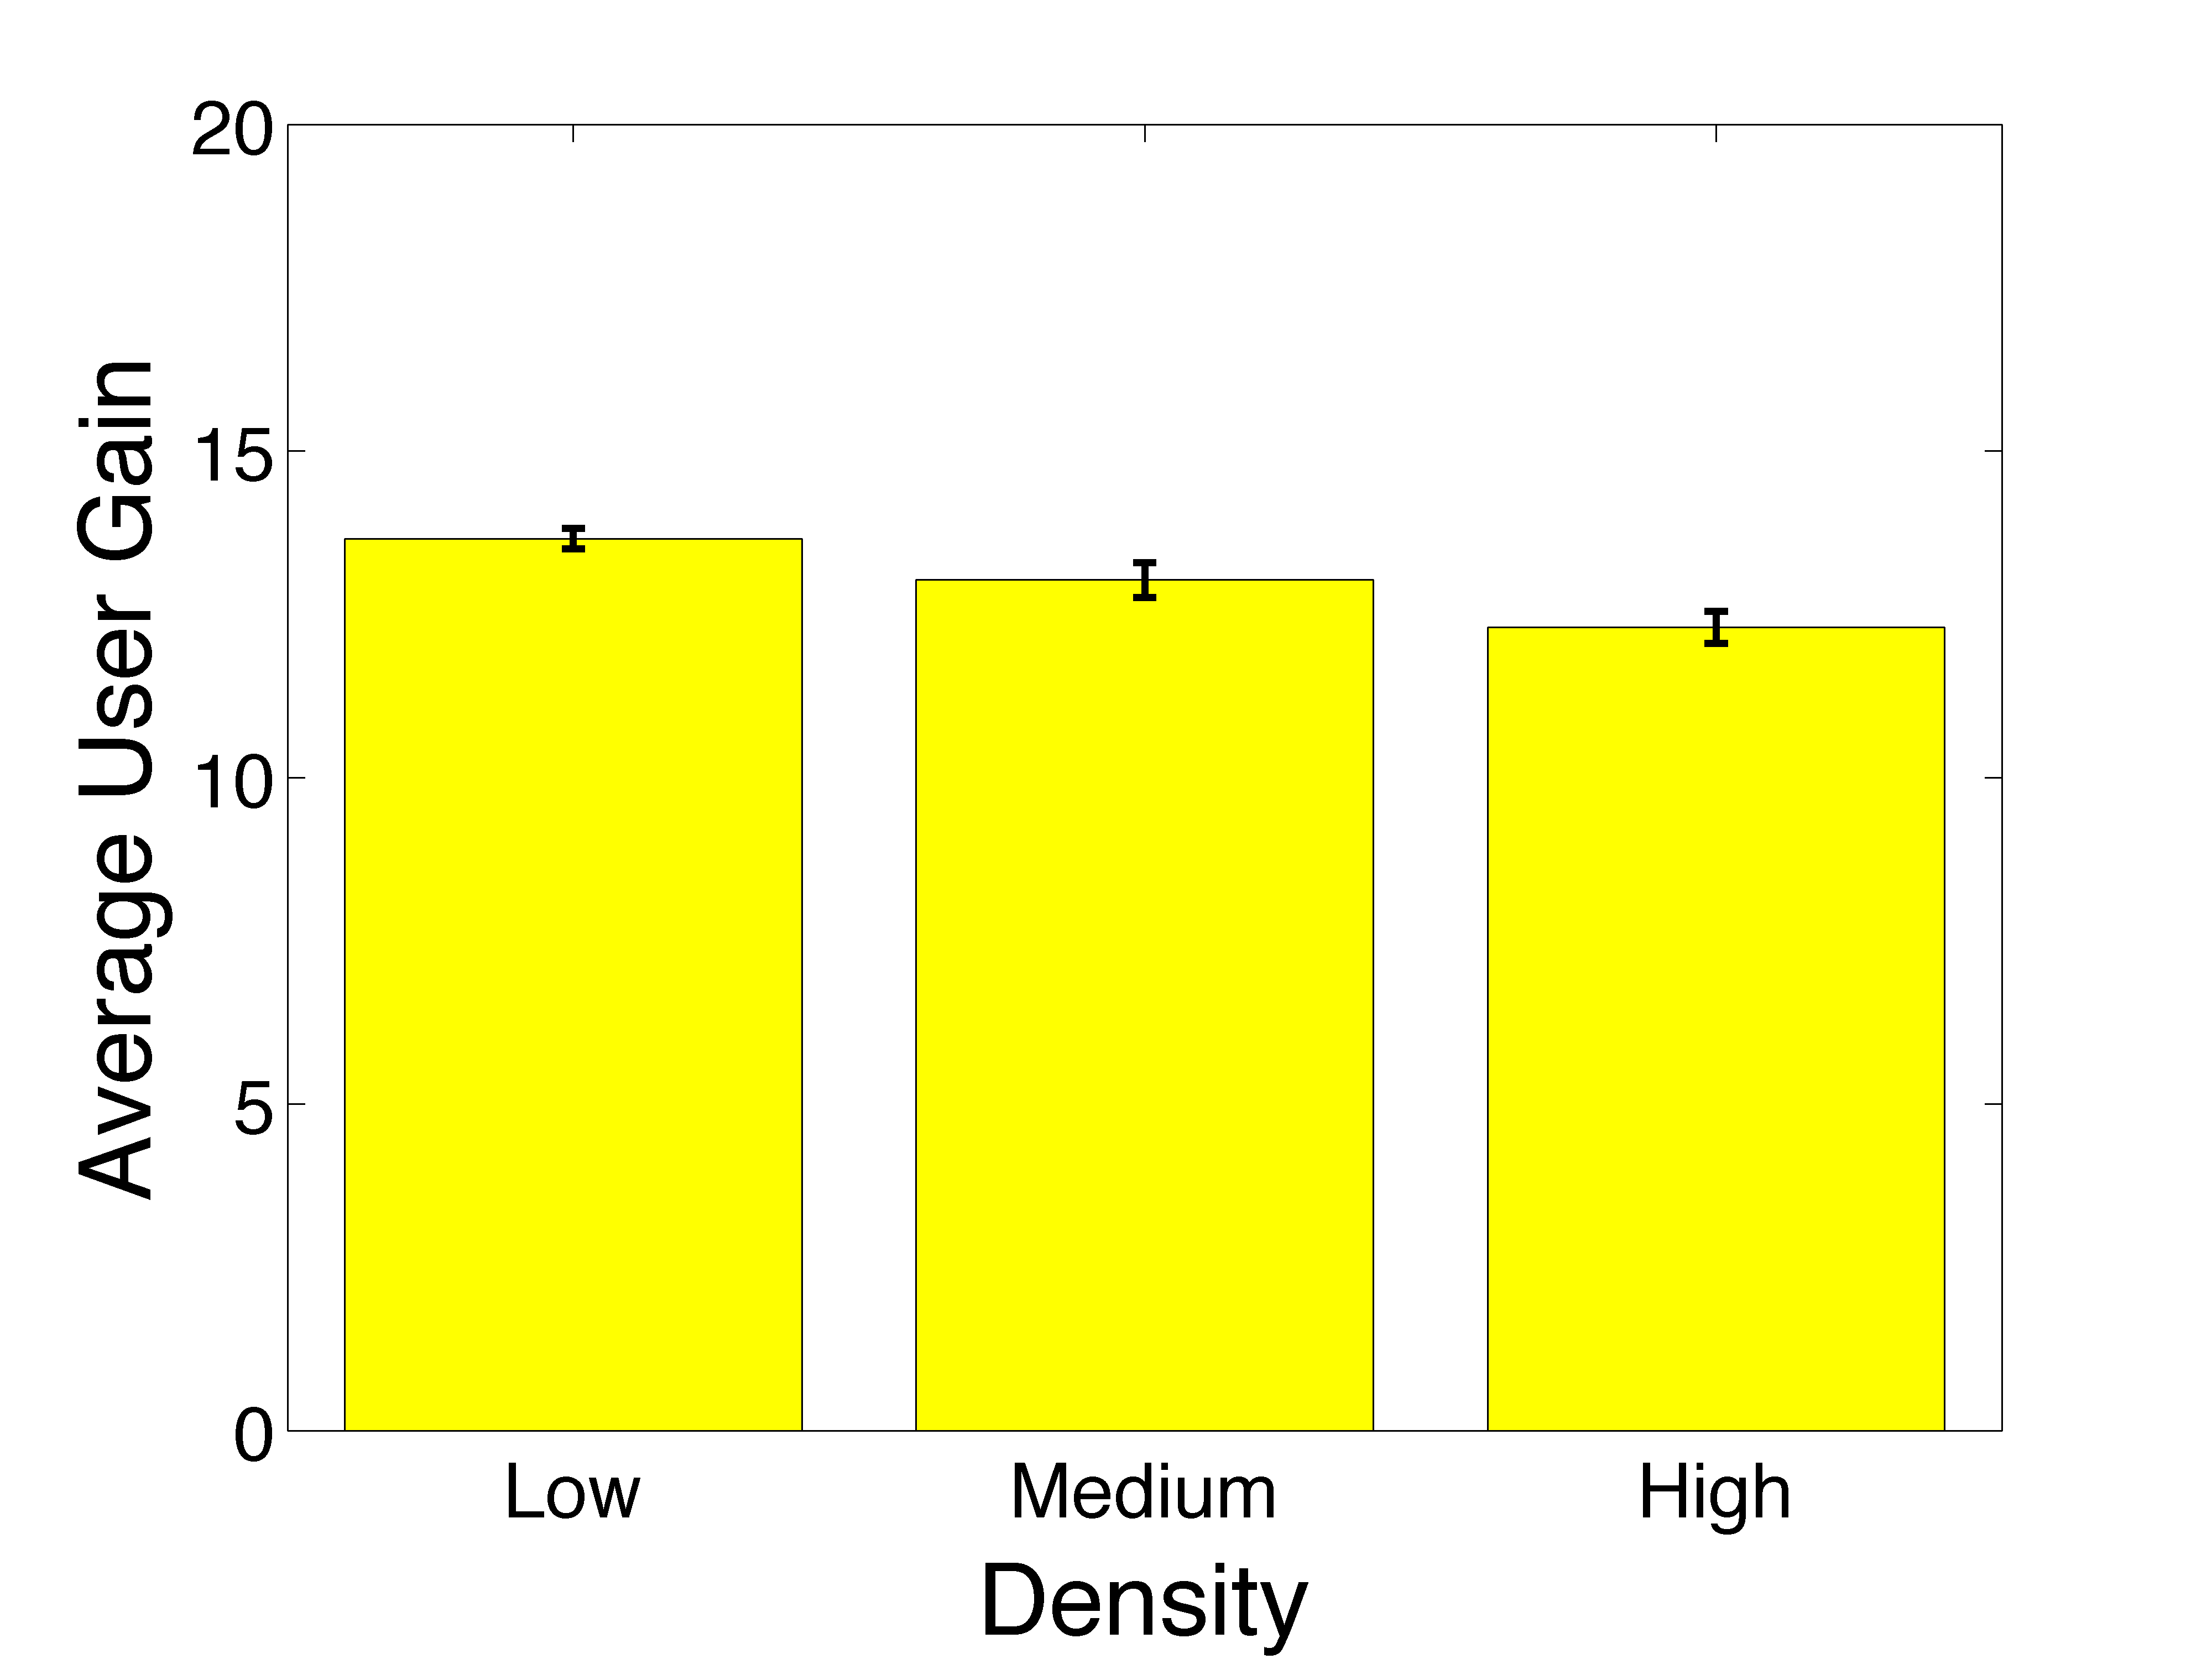
\includegraphics[width=0.33\textwidth,type=png,ext=.png,read=.png]{img/ScaleFree-1.000-AUG}
% 	}  
%   \hspace{-0.1in}\subfigure[Small World.]{
%   	%\label{fig:res_mmuca_time}
% 	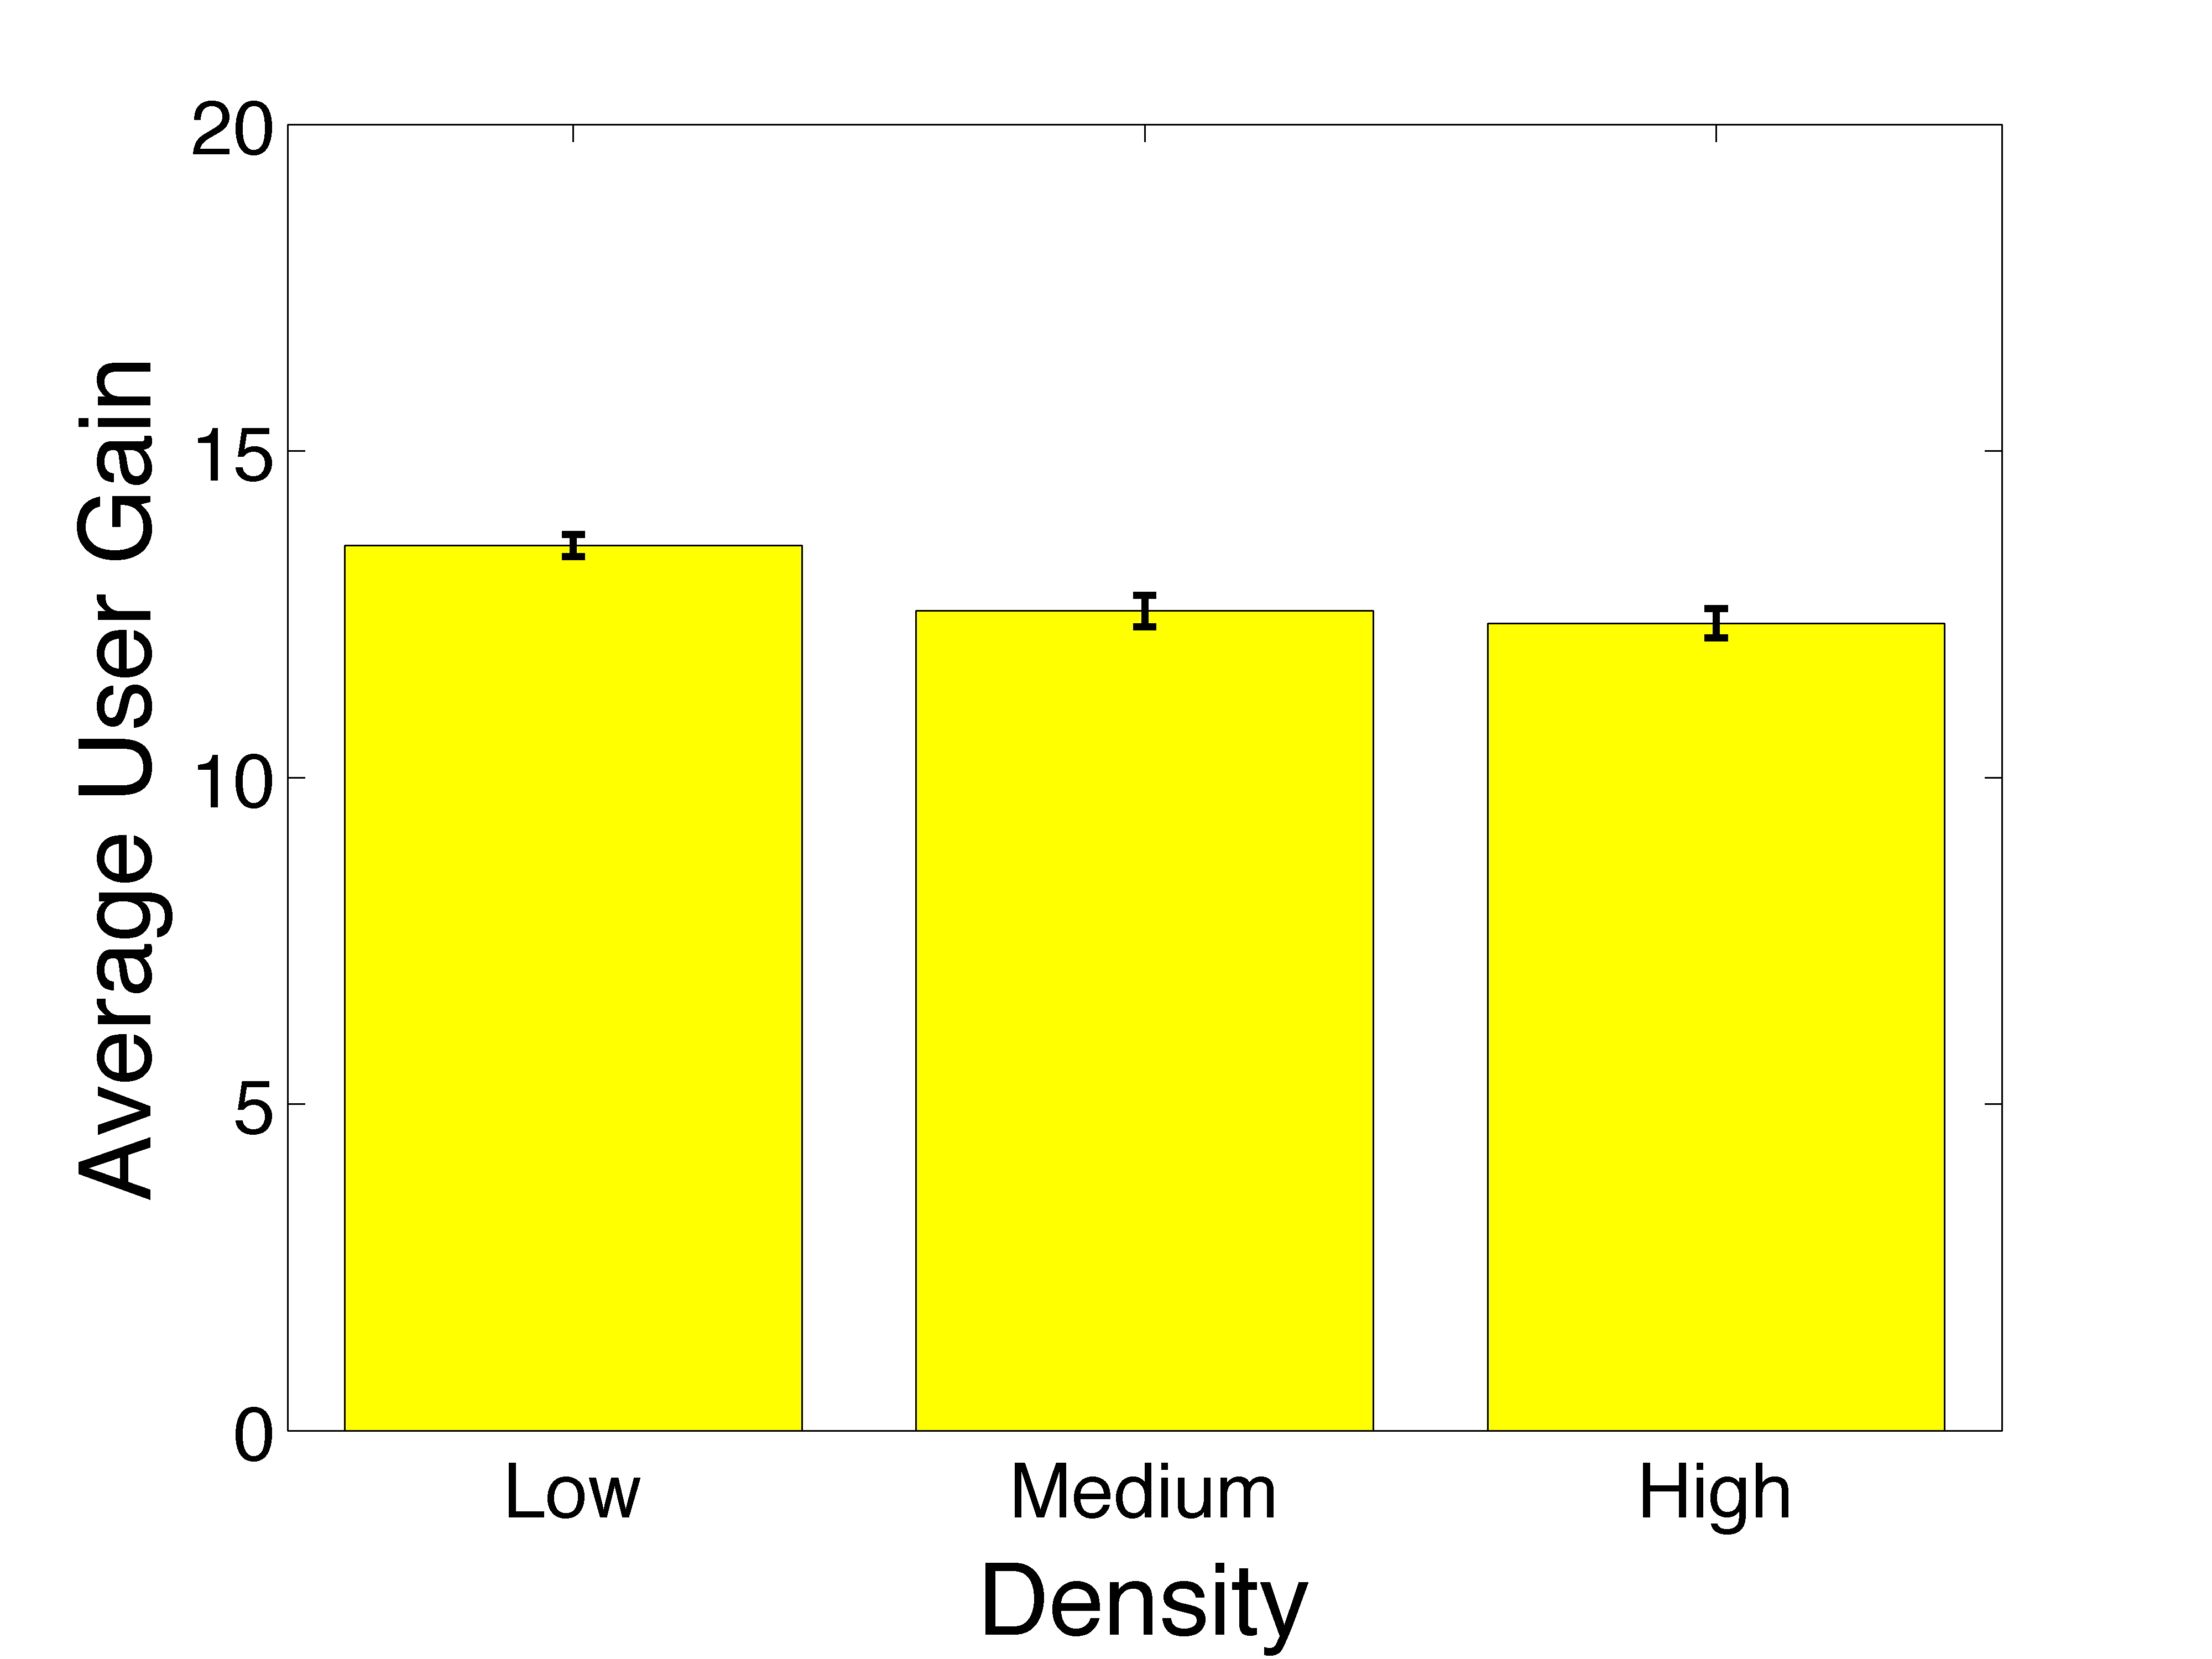
\includegraphics[width=0.33\textwidth,type=png,ext=.png,read=.png]{img/SmallWorld-1.000-AUG}
% 	}    
%   \caption{$70/80 p=1$ Graphs showing the average percent gain of consumers'
%   payoffs in the coalitions with respect to the payoff of individual coalitions on
%   different topologies and with different densities. }
%   \label{fig:graphs_gain}
% \end{figure*}
\subsubsection{Consumer's gain}

In this section we analyse the consumer's gain that agents obtain in our model
on the different network and market configurations. Let $\rho_i$ be the payment
of agent $a_i\in A$ in a coalition and $v(\{i\})$ the payment of the agent in its single coalition. Then, the average percent
consumer gain is assessed as $\frac{\sum_{a_i\in A} \rho_i - v(\{i\})}{\vert A
\vert}$. Figure \ref{fig:graphs_gain} show the results
for 12 agents on a random, scalefree and smallworld networks in the three
different market scenarios respectively.
We also plotted the standard error of the mean as a measure of the
variance in each graph. Only data regarding instances with non-empty core are
plotted. Observe that in all configurations, although the average percent user
gain is increased with density, this increment is not significant. Moreover, the
average percent user gain is much higher (around $10\%$) in M3 market than not
in M1 and M2 (around $1\%$).

% Each graph shows the
% mean
%among the from 50 problem instances that resulted in non-empty core of the user
%percent gain of consumers in coalitions with respect to their individual
%coalitions when varying the density of the agent's social network.

%As expected graphs show that increasing the network social density increases
% the percent user gain in all scenarios because each new link allows the formation of
%a set of new energy coalitions that were forbidden before. However this
%increment of gain is more significant on random graphs and small world networks
%where the degree of nodes is more uniform than not in scale free due to the
%presence of hubs.
Table \ref{tab:percentage_core_emptiness} shows the percentage of
instances under each configuration for which the core was detected as empty.
Notice that in all network topologies, the number of instances for which the core is empty
increases with the density of the network. These results are coherent with the
well-known results that any acyclic network (which has by definition the
lowest density) is guarantee to have a non-empty core \cite{demange2004}. As we
increase the density the number of cycles also increase and results show that the probability
of core emptiness is higher.
Regarding different network topologies, we observe that the number of instances
with core emptiness is higher in scale free networks, where the links are
concentrated on hubs, than not on random and small-world networks, where each
node in average have the same degree.
Finally, we also observe that the number of instances with core empty is much
higher on M1 and M2 than not in M3. Although we need to perform a deeper
analysis on these results, they lead to the hypothesis that the more the
distance of prices in the market the less the probability of having an empty
core in the coalitional game.



\begin{figure*}  
  \centering  
  \hspace{-0.1in}\subfigure[Random Graphs M1.]{
	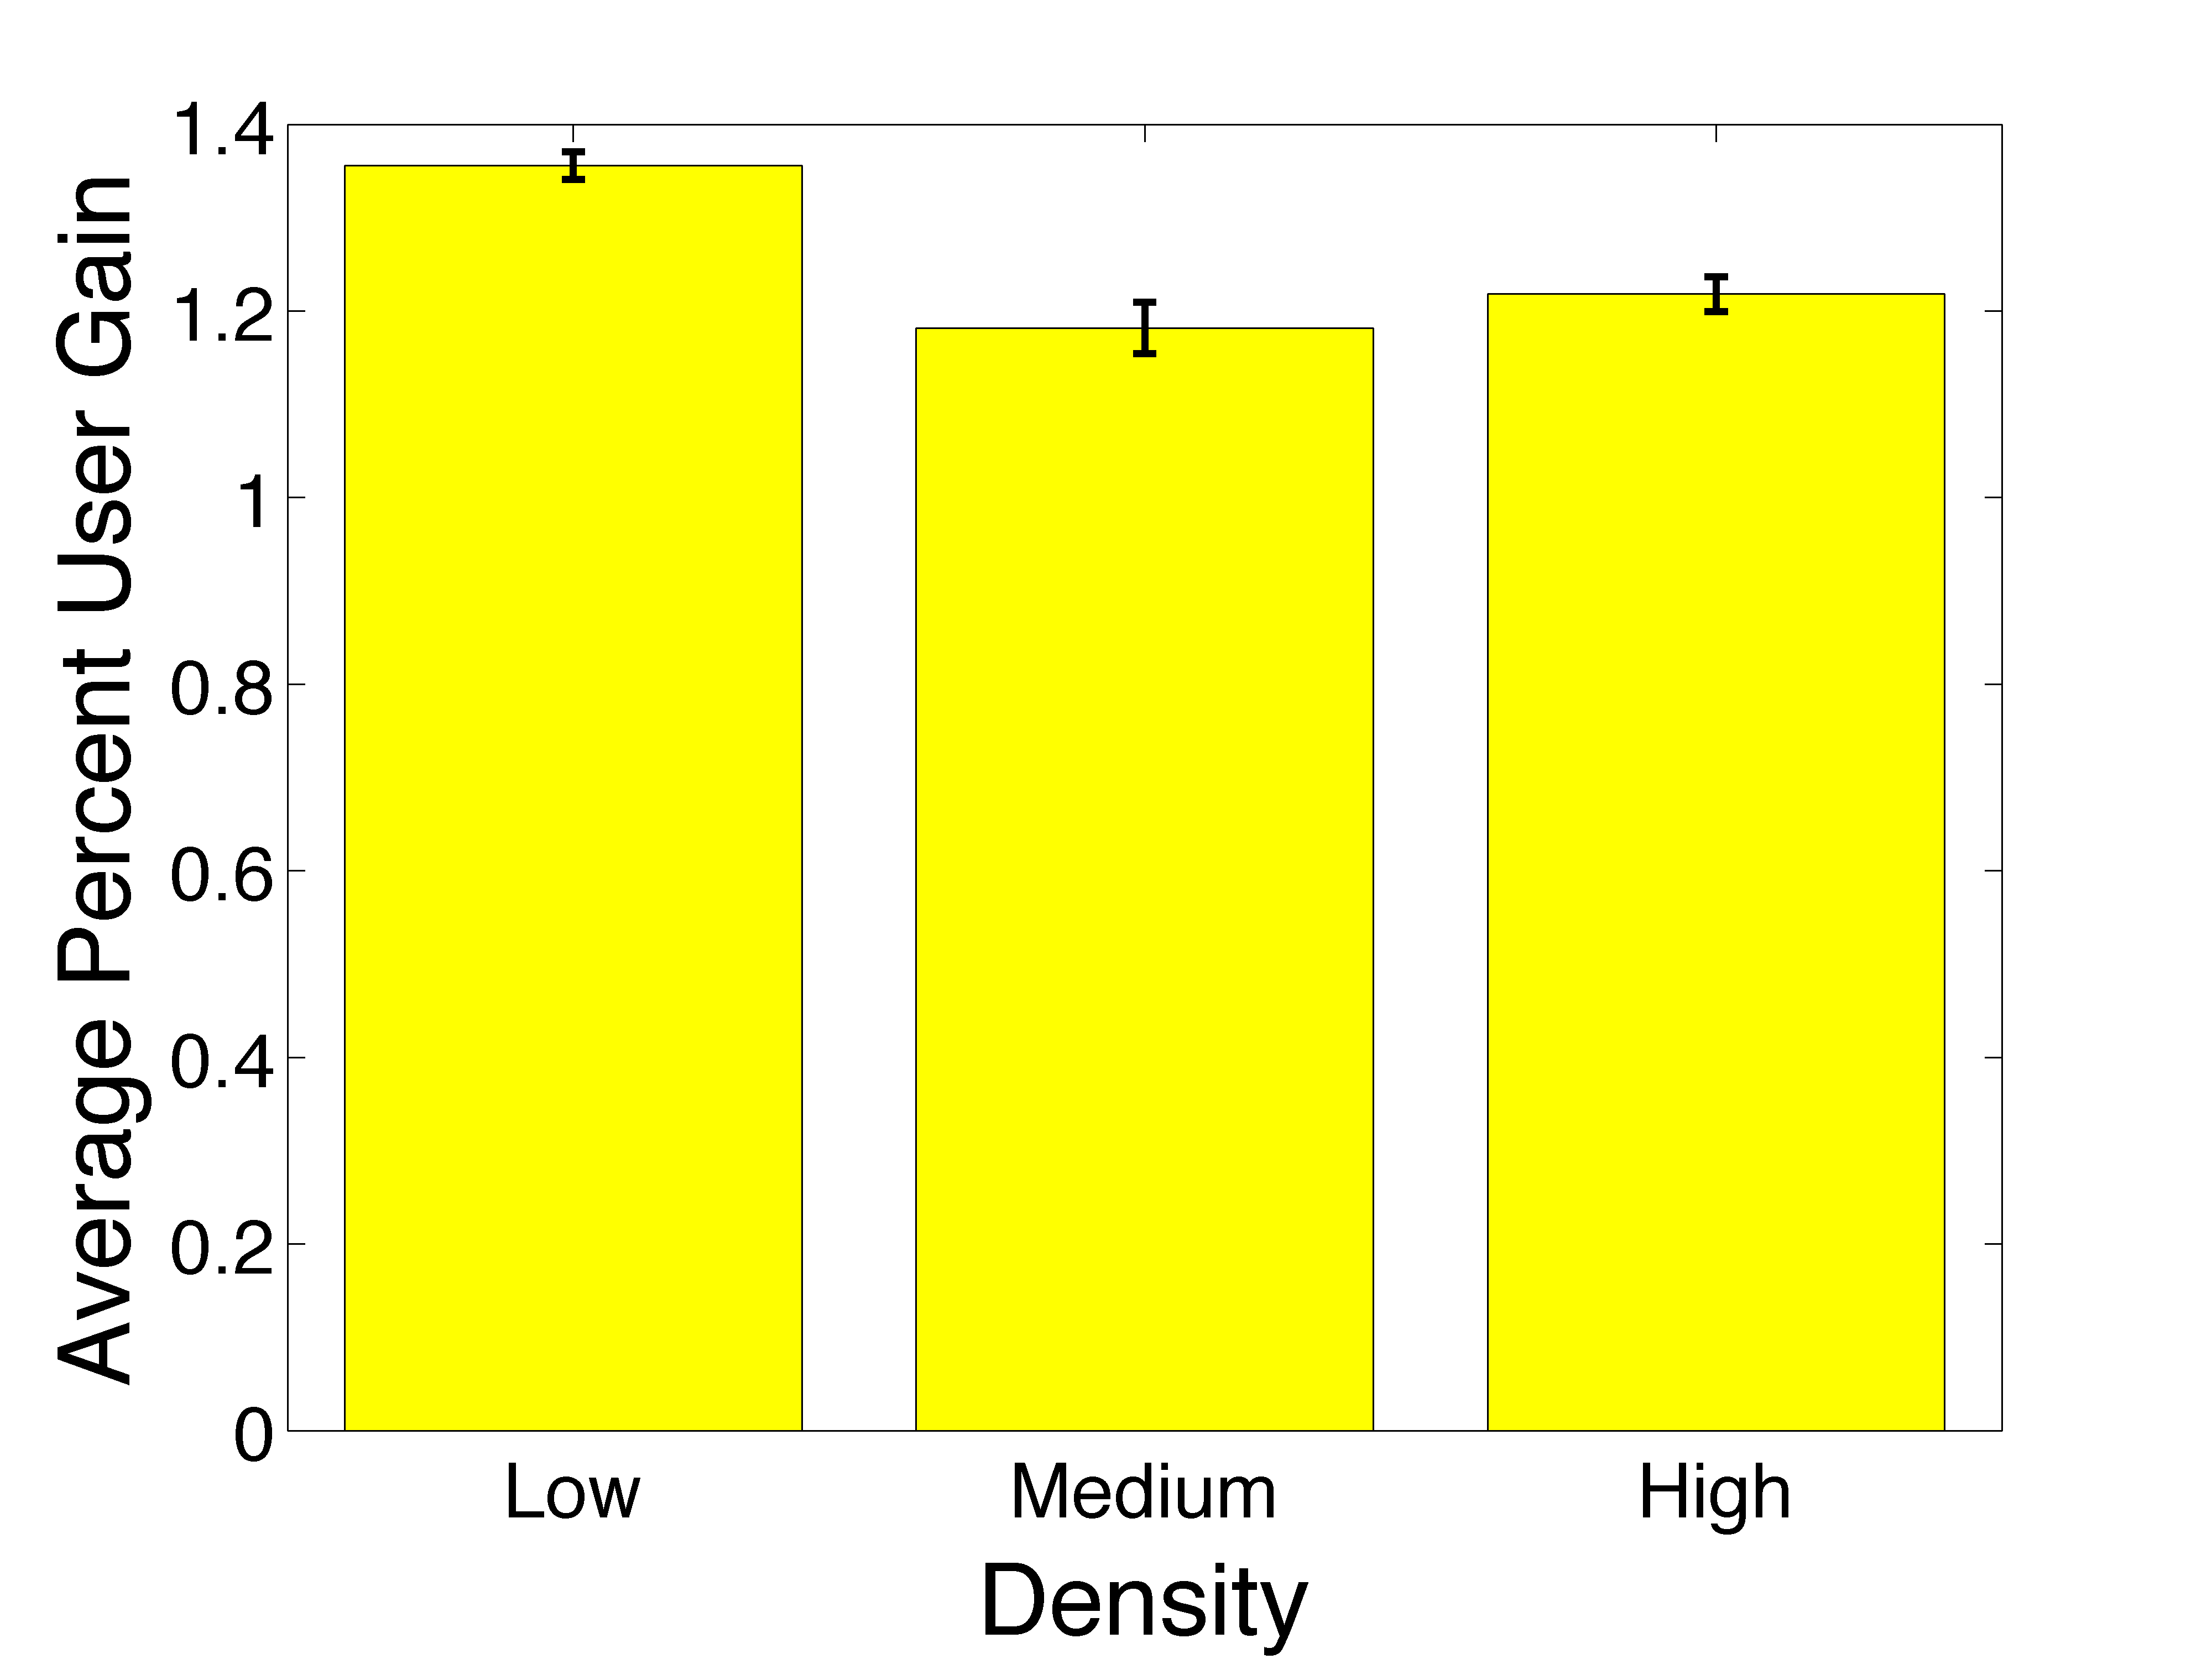
\includegraphics[width=0.33\textwidth,type=png,ext=.png,read=.png]{img/Random-1.000-AUG-PER}
	}  
  \hspace{-0.1in}\subfigure[Scale Free M1.]{
	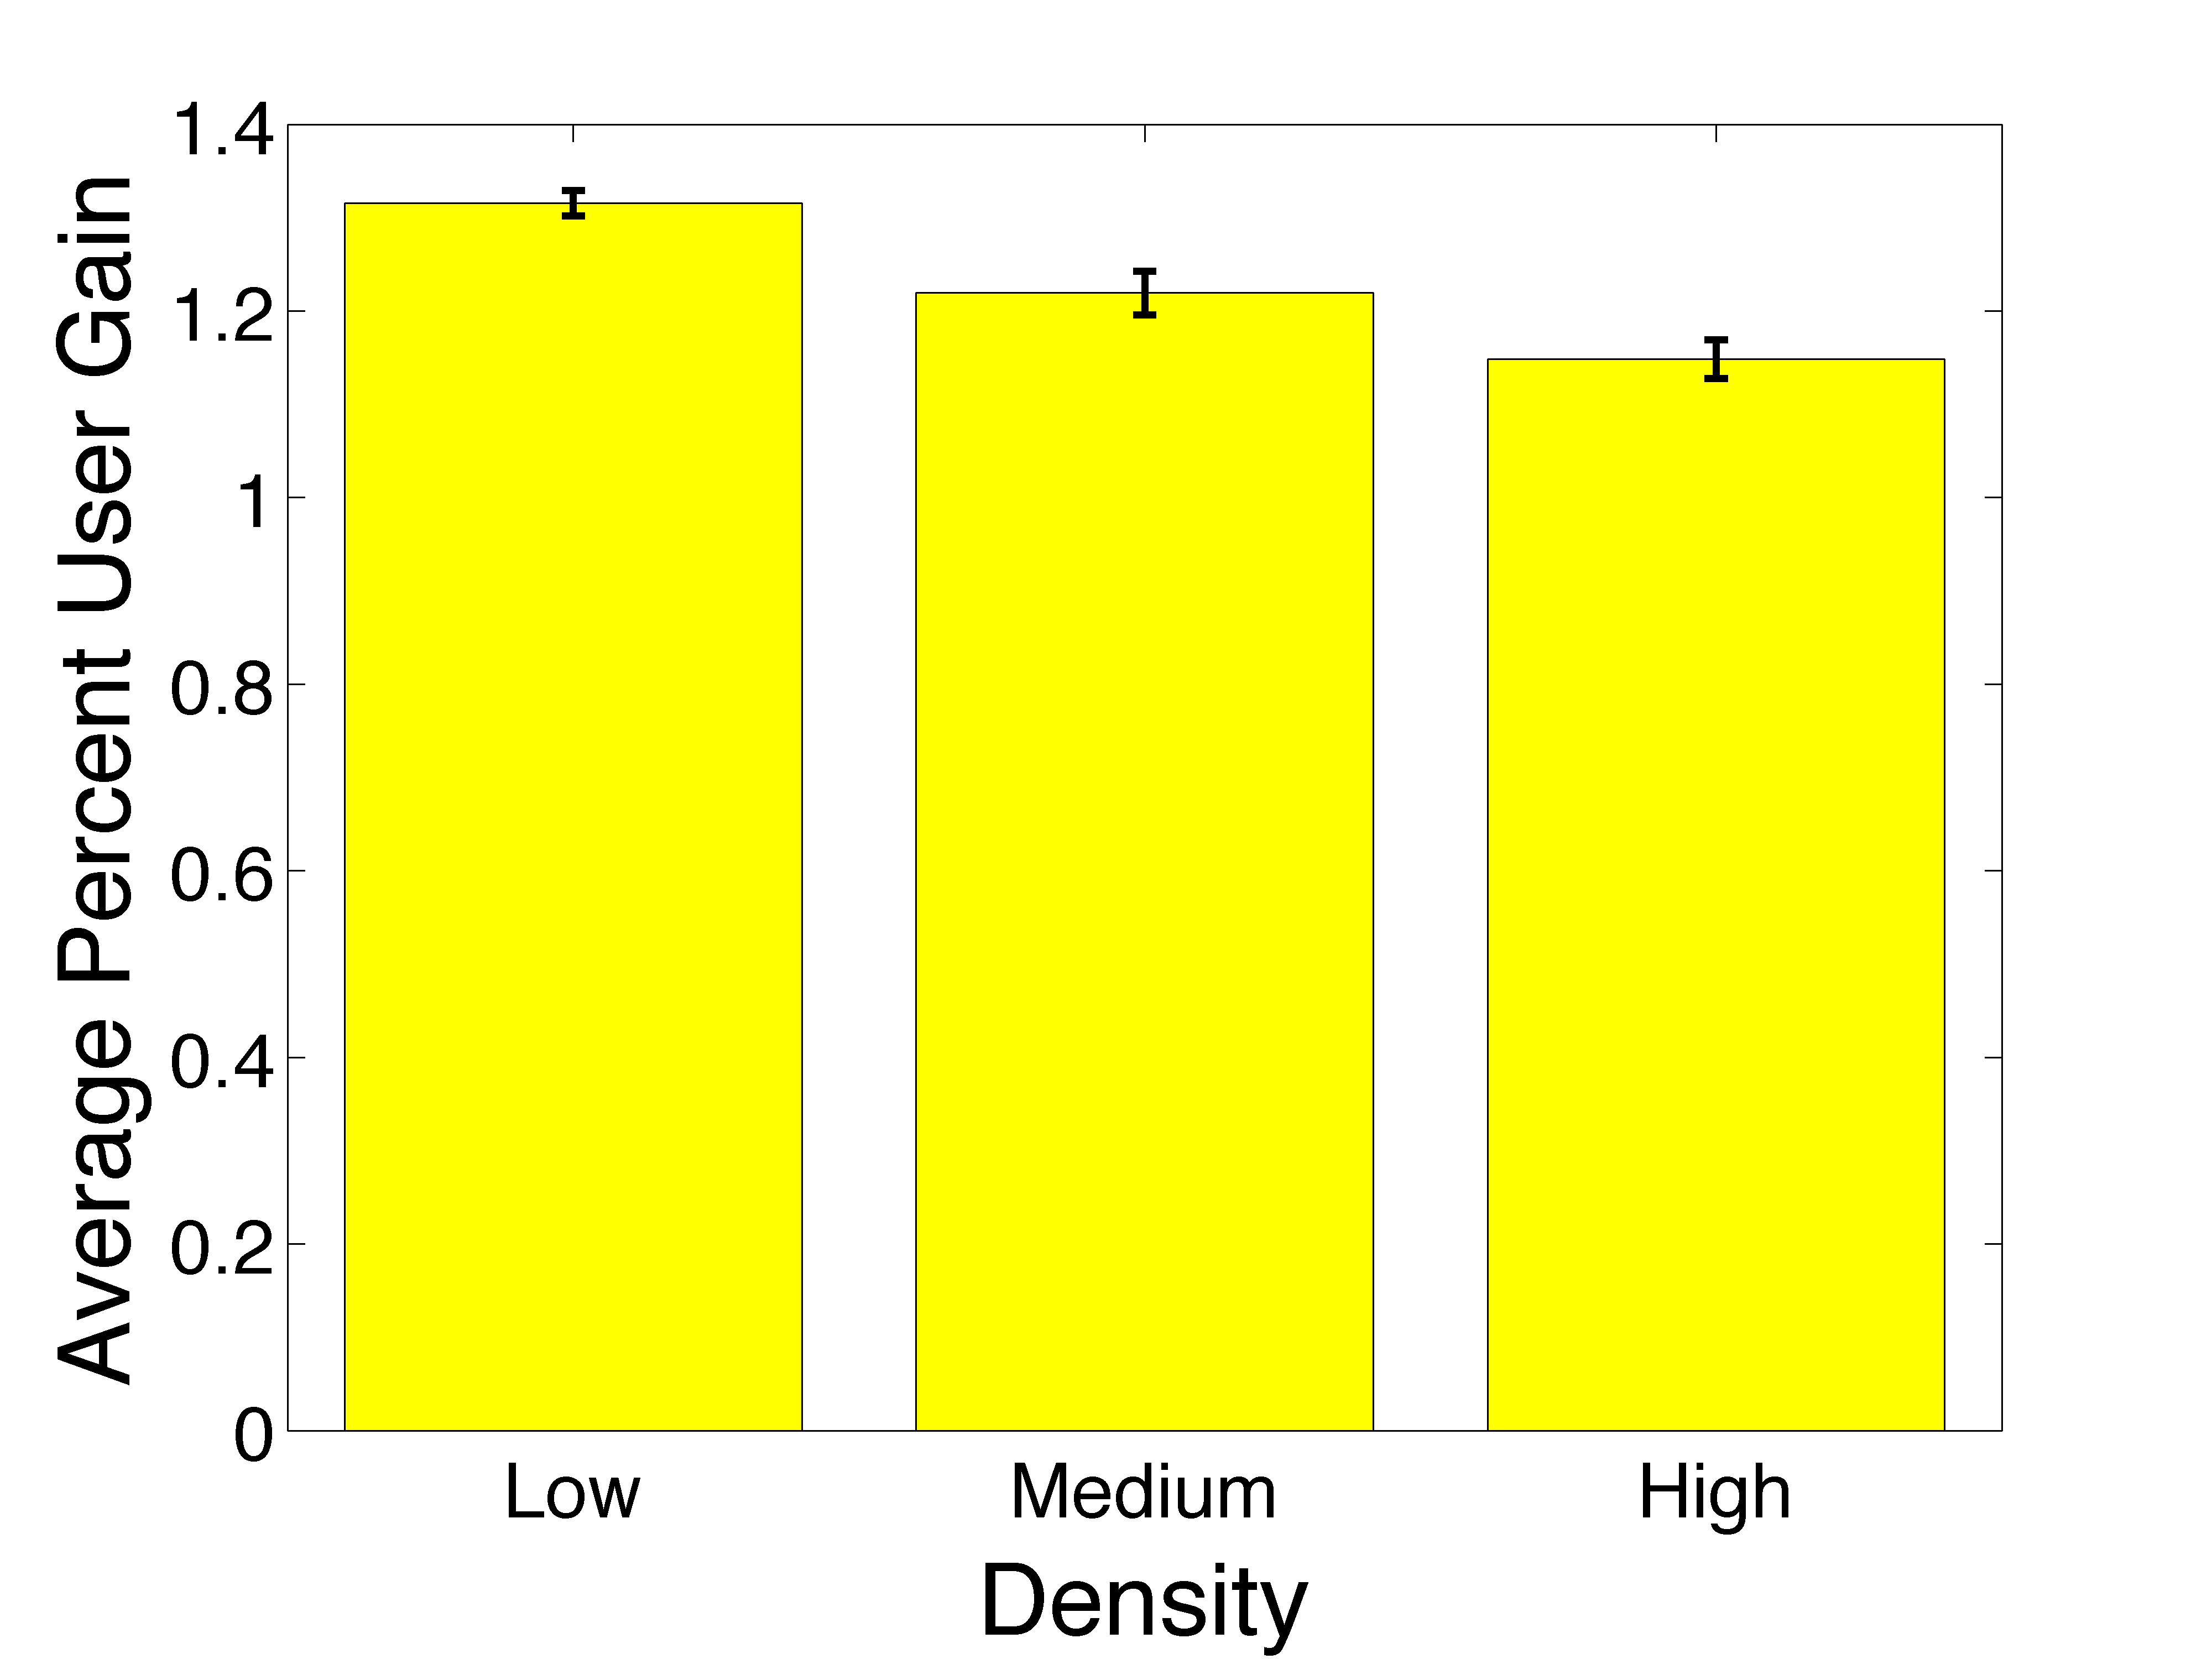
\includegraphics[width=0.33\textwidth,type=png,ext=.png,read=.png]{img/ScaleFree-1.000-AUG-PER}
	}  
  \hspace{-0.1in}\subfigure[Small World M1.]{
	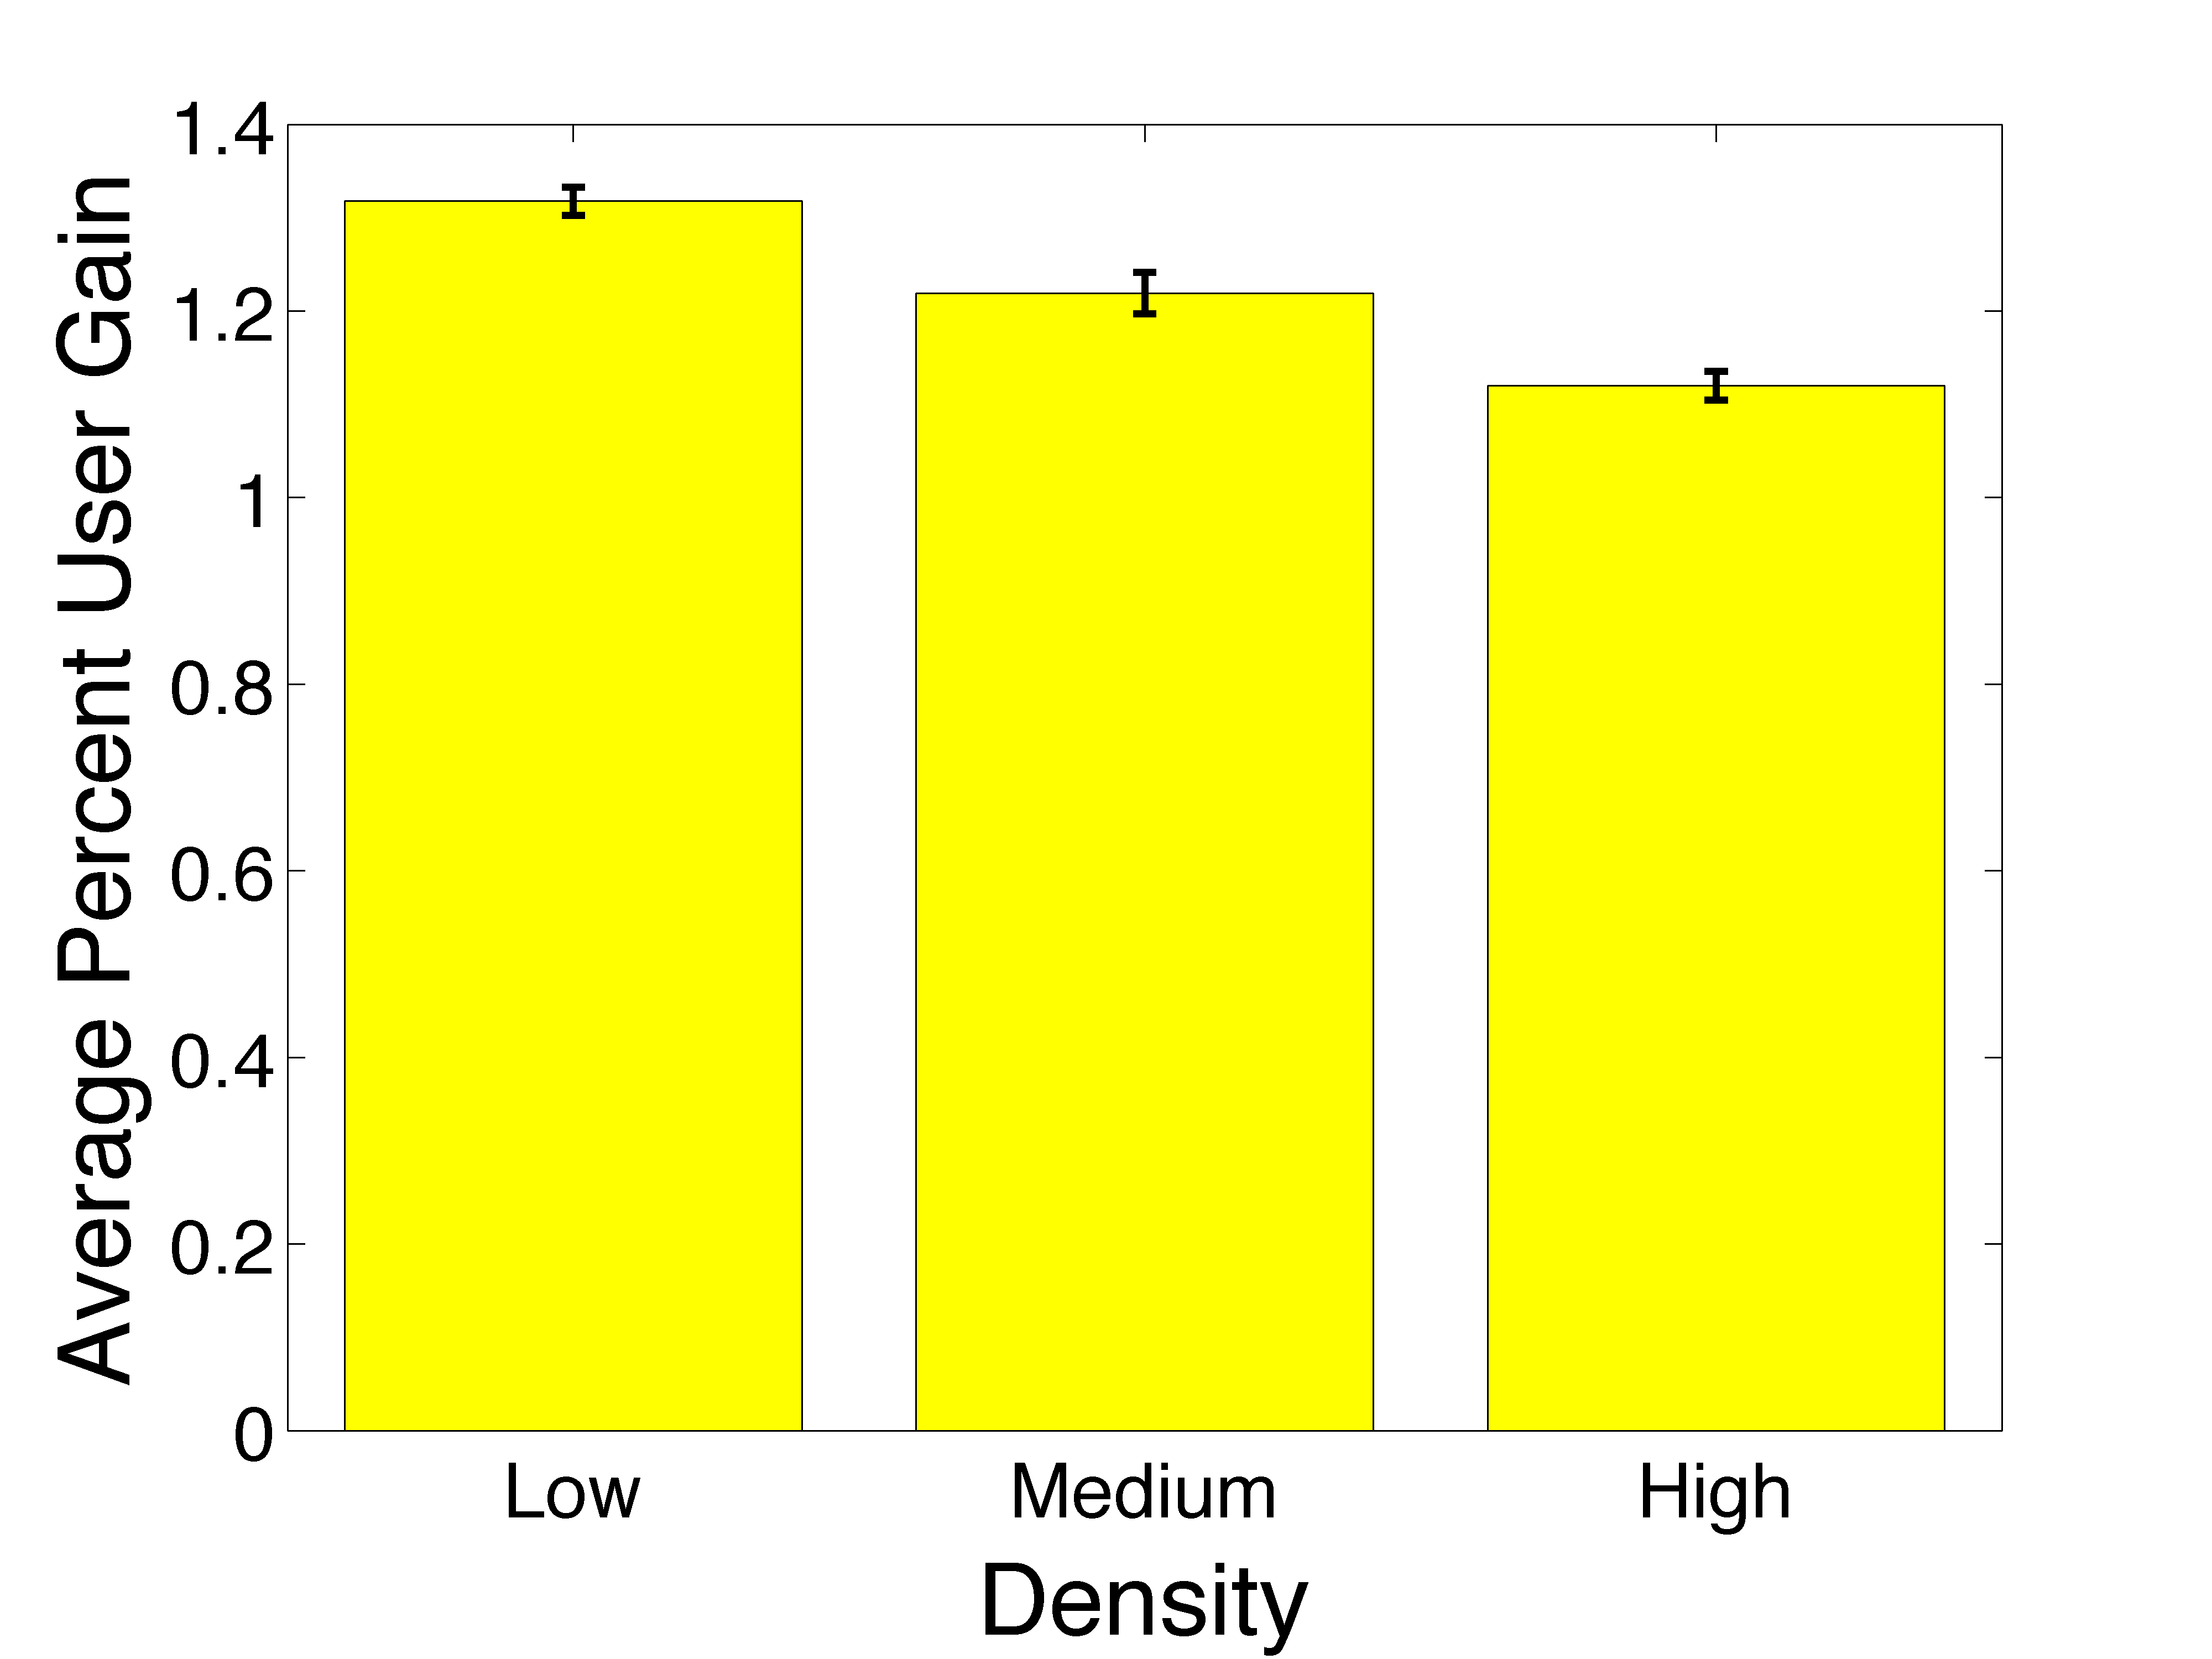
\includegraphics[width=0.33\textwidth,type=png,ext=.png,read=.png]{img/SmallWorld-1.000-AUG-PER}
	}  
  \hspace{-0.1in}\subfigure[Random Graphs M2.]{
	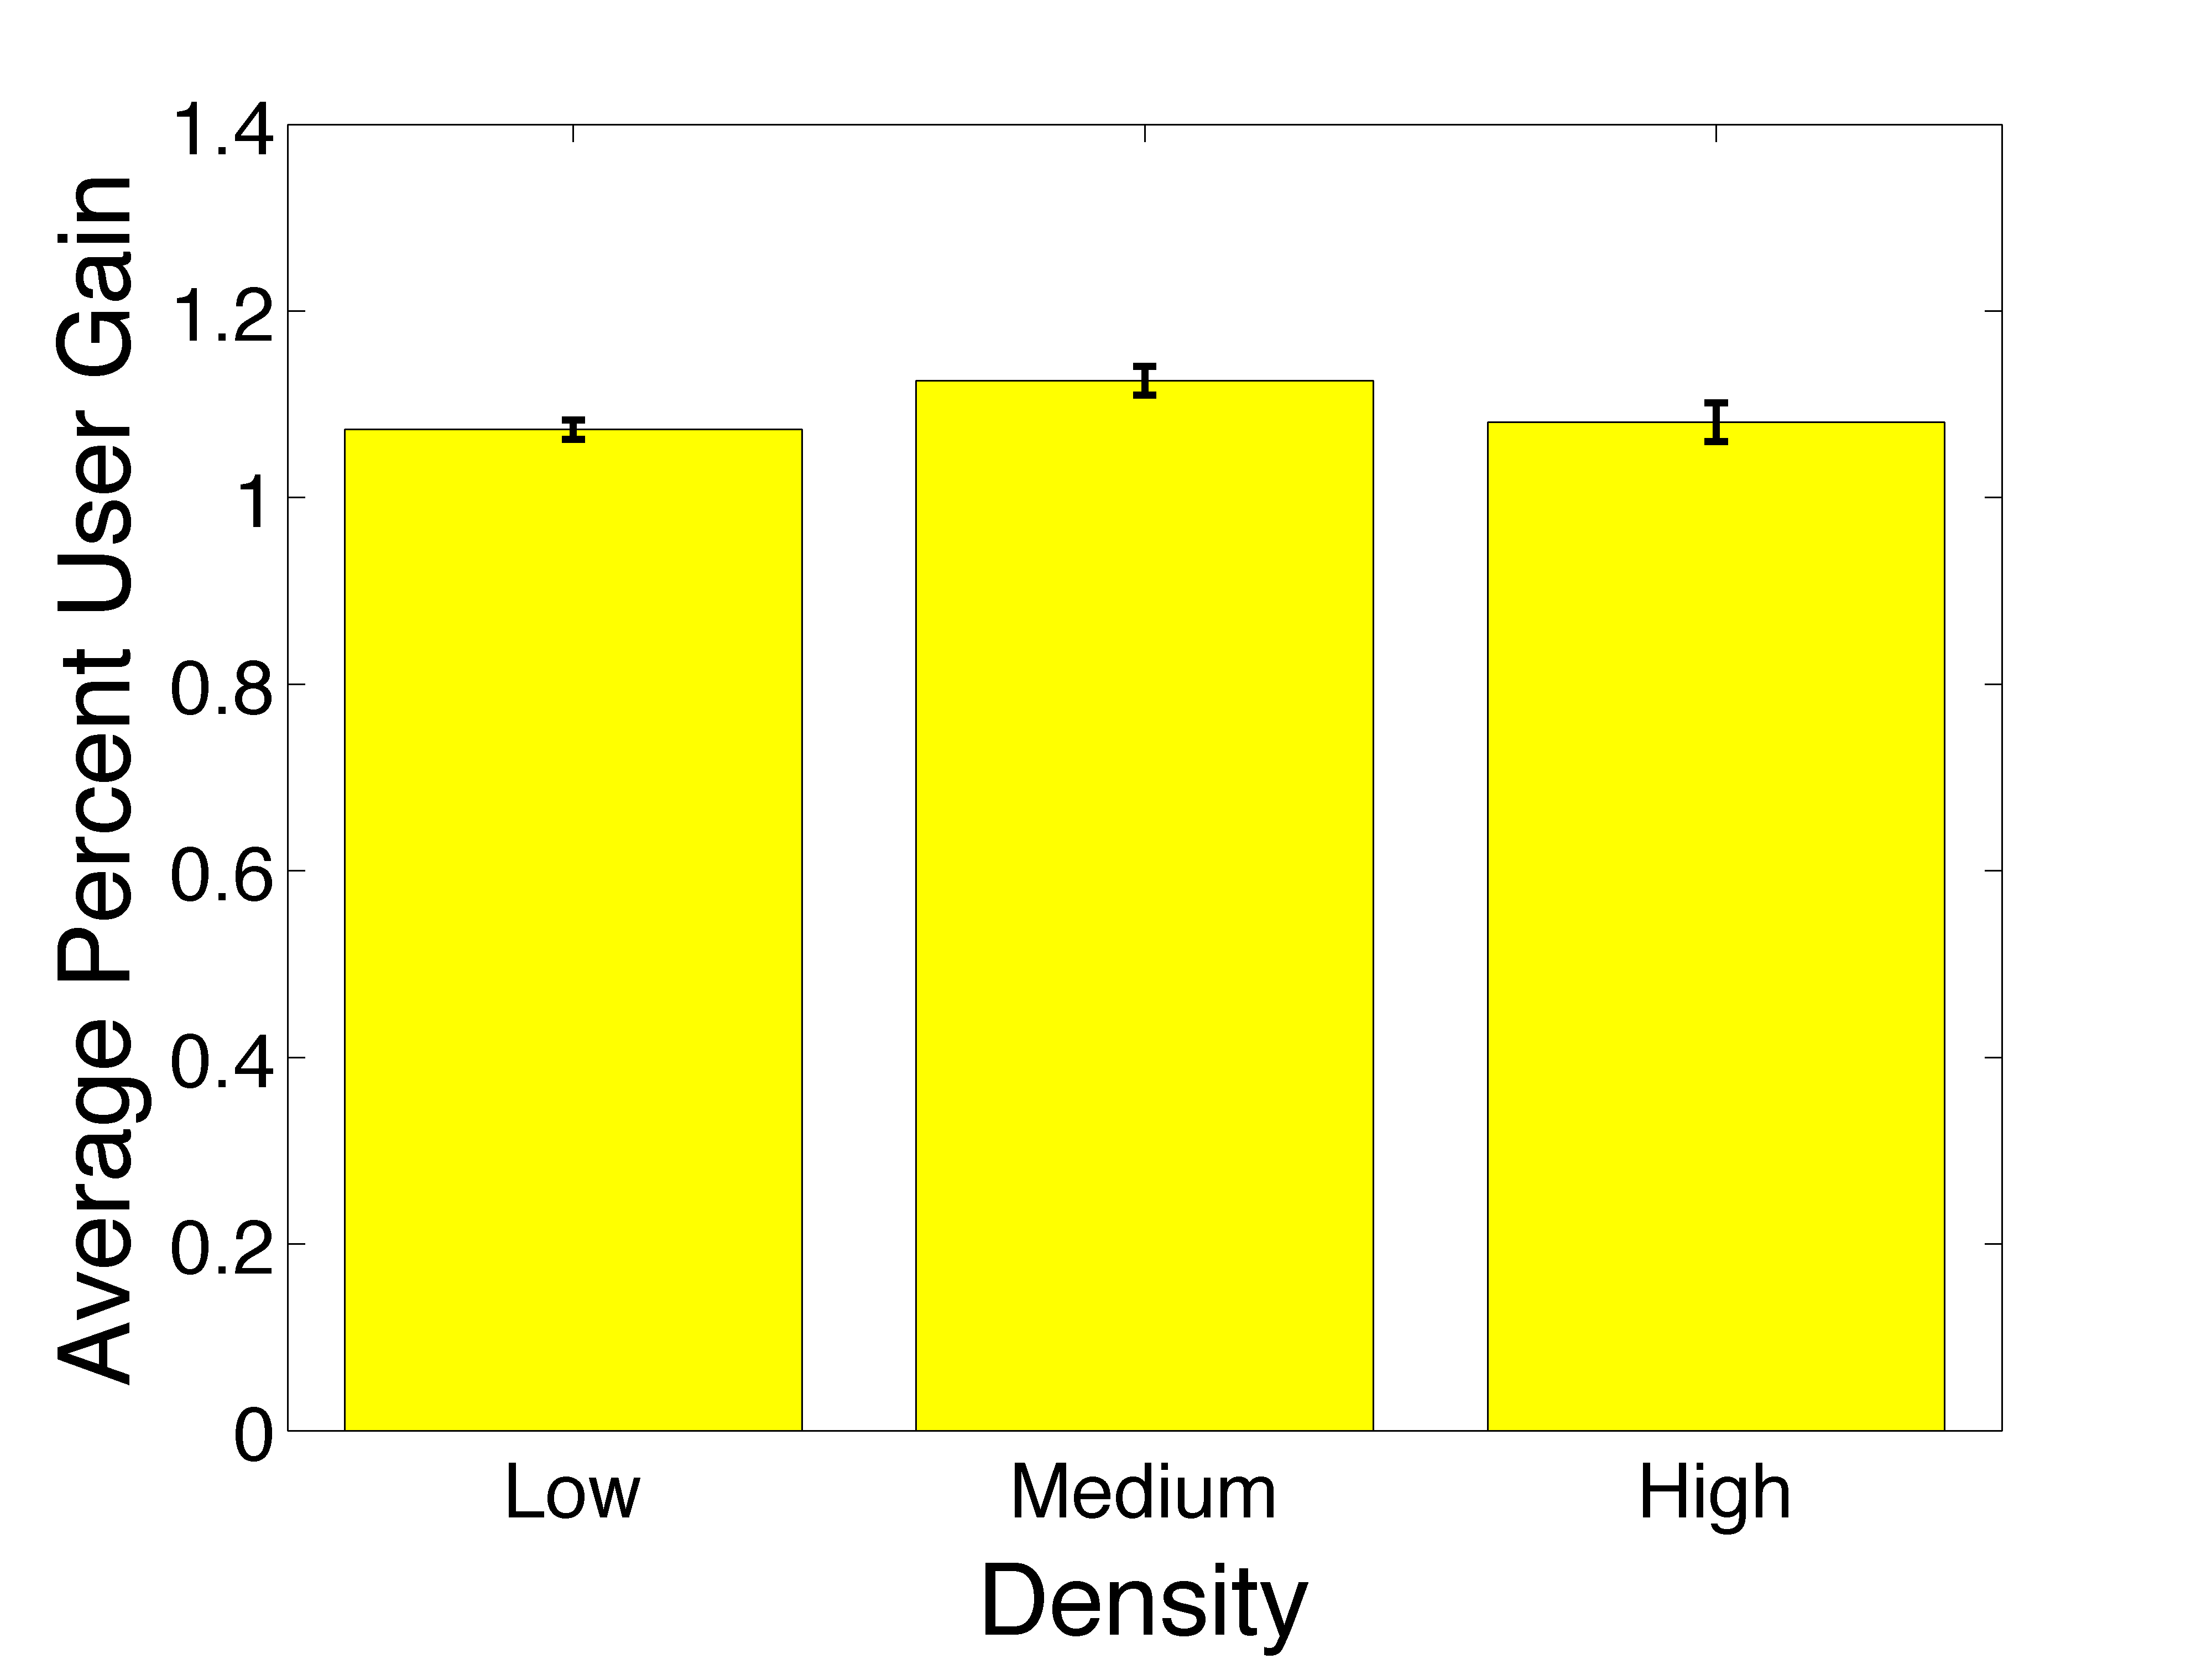
\includegraphics[width=0.33\textwidth,type=png,ext=.png,read=.png]{img/Random-0.875-AUG-PER}
	}  
  \hspace{-0.1in}\subfigure[Scale Free M2.]{
	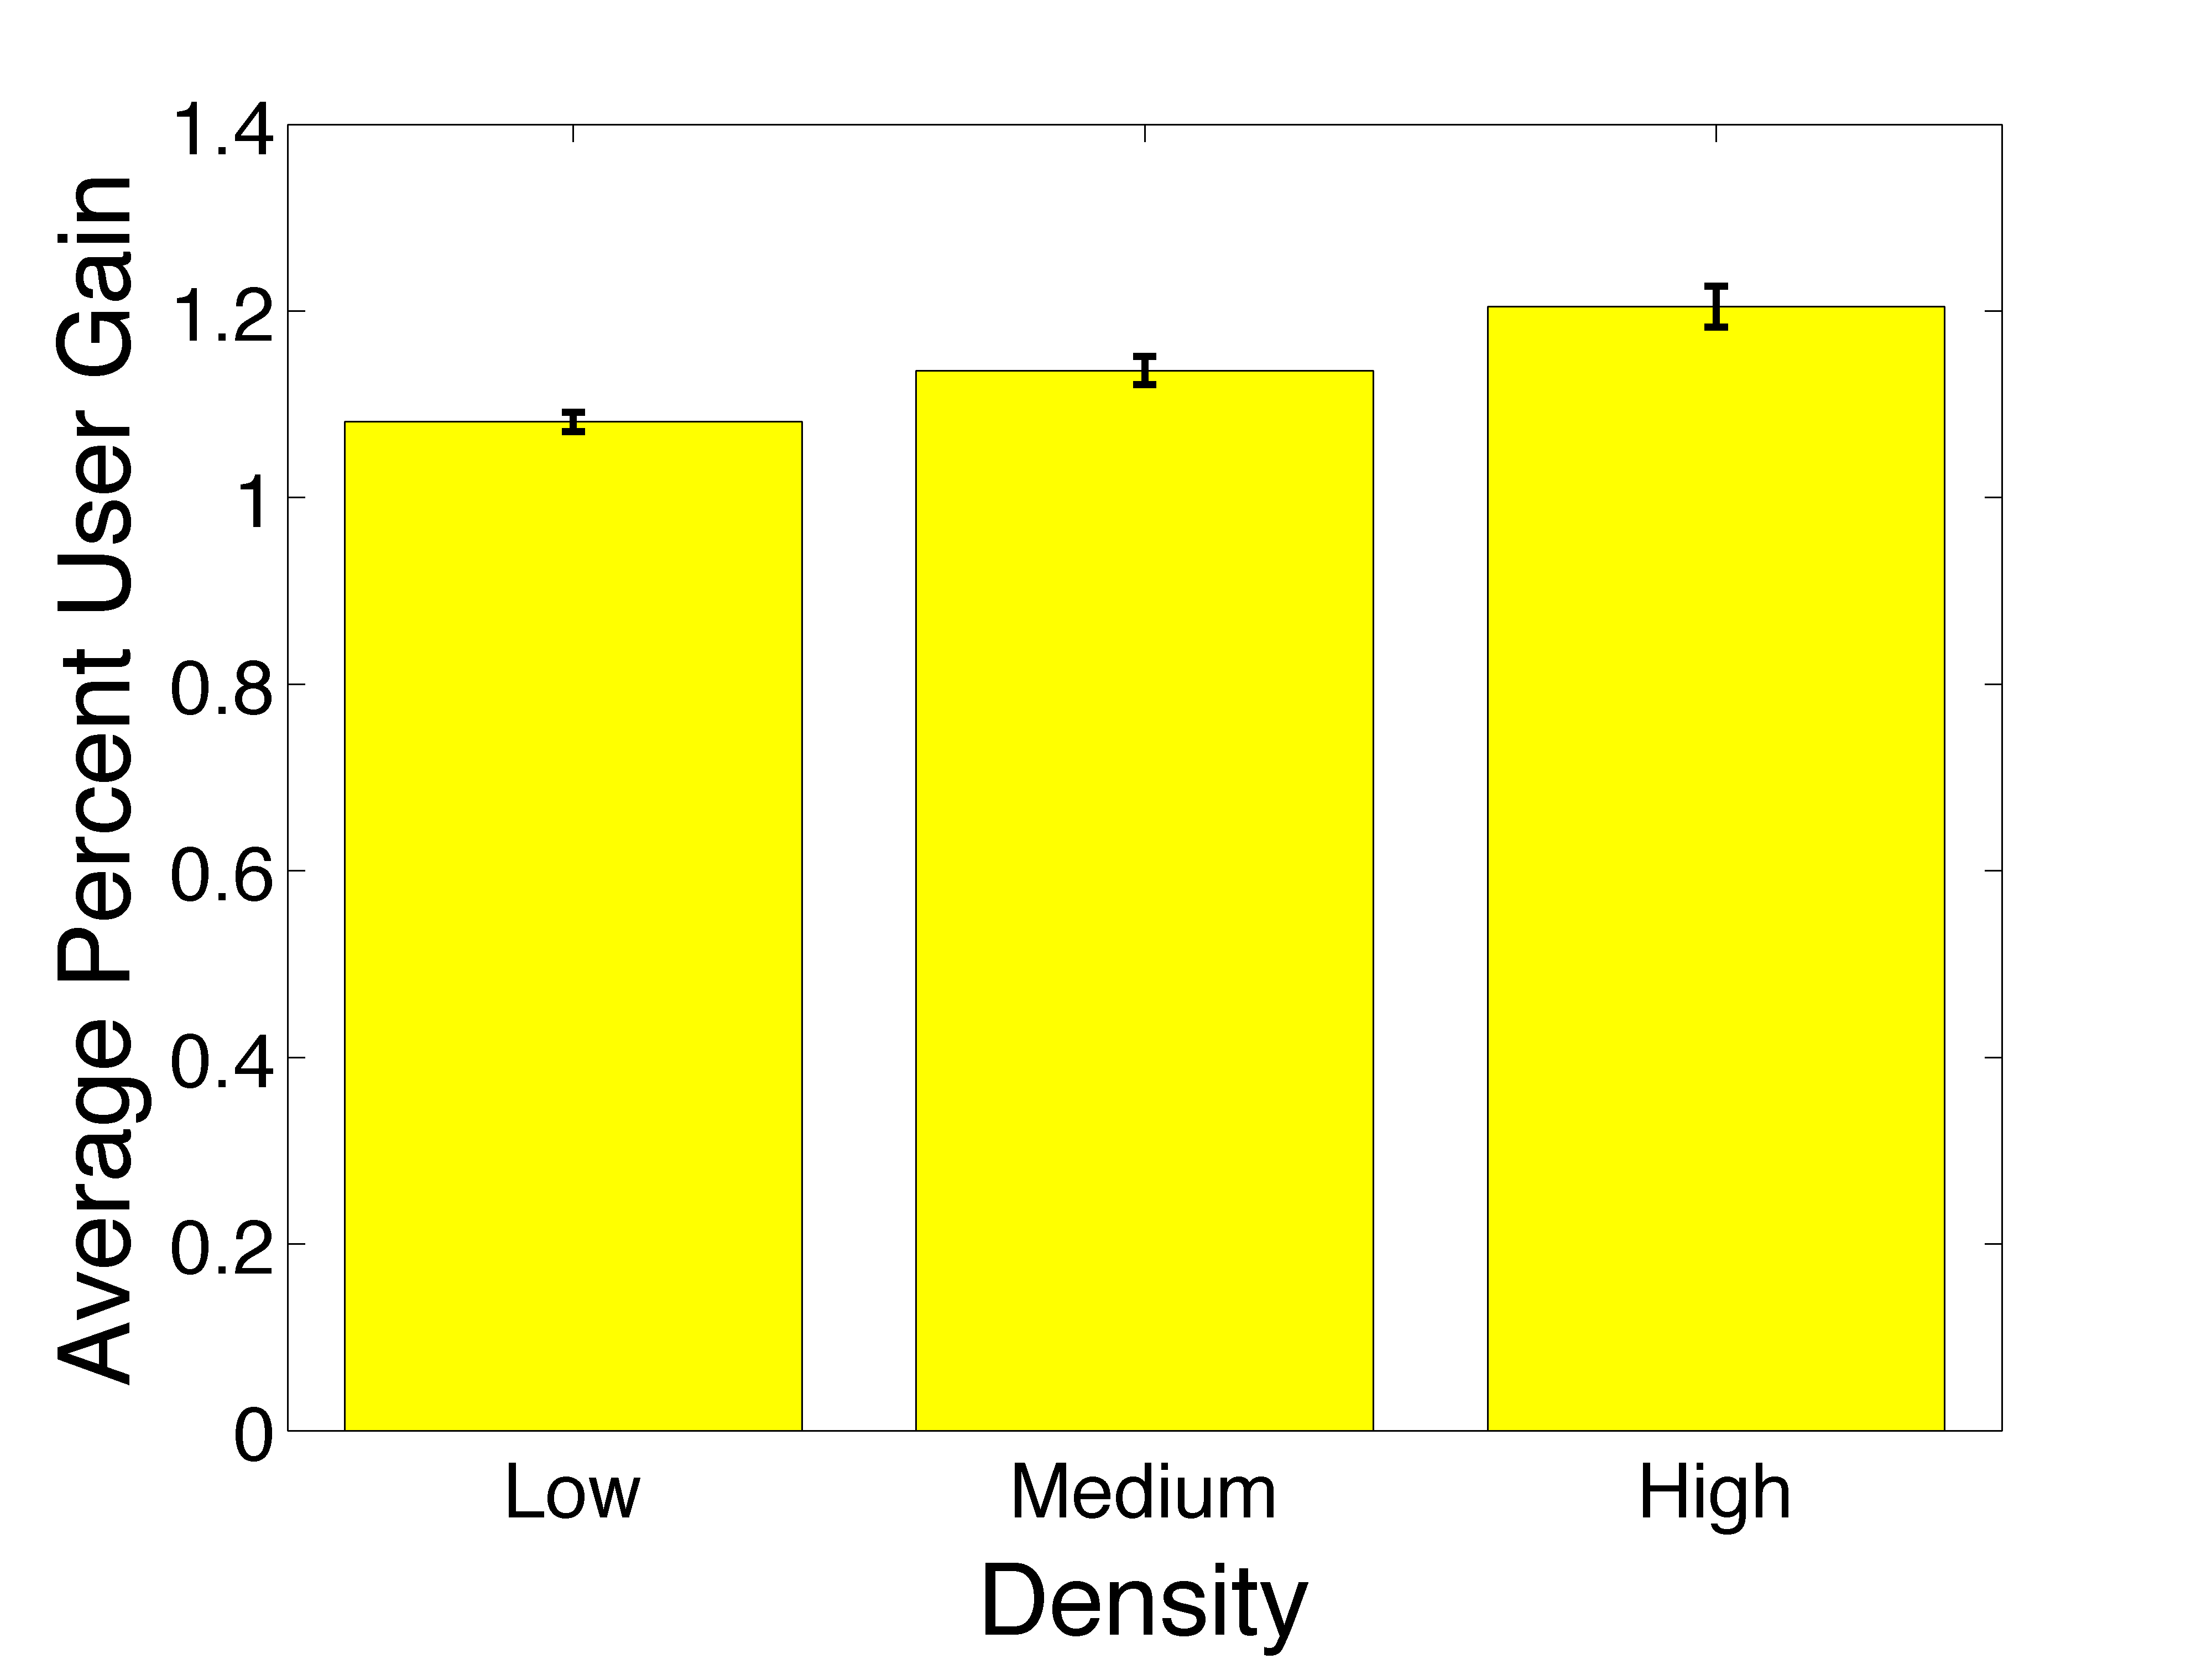
\includegraphics[width=0.33\textwidth,type=png,ext=.png,read=.png]{img/ScaleFree-0.875-AUG-PER}
	}  
  \hspace{-0.1in}\subfigure[Small World M2.]{
	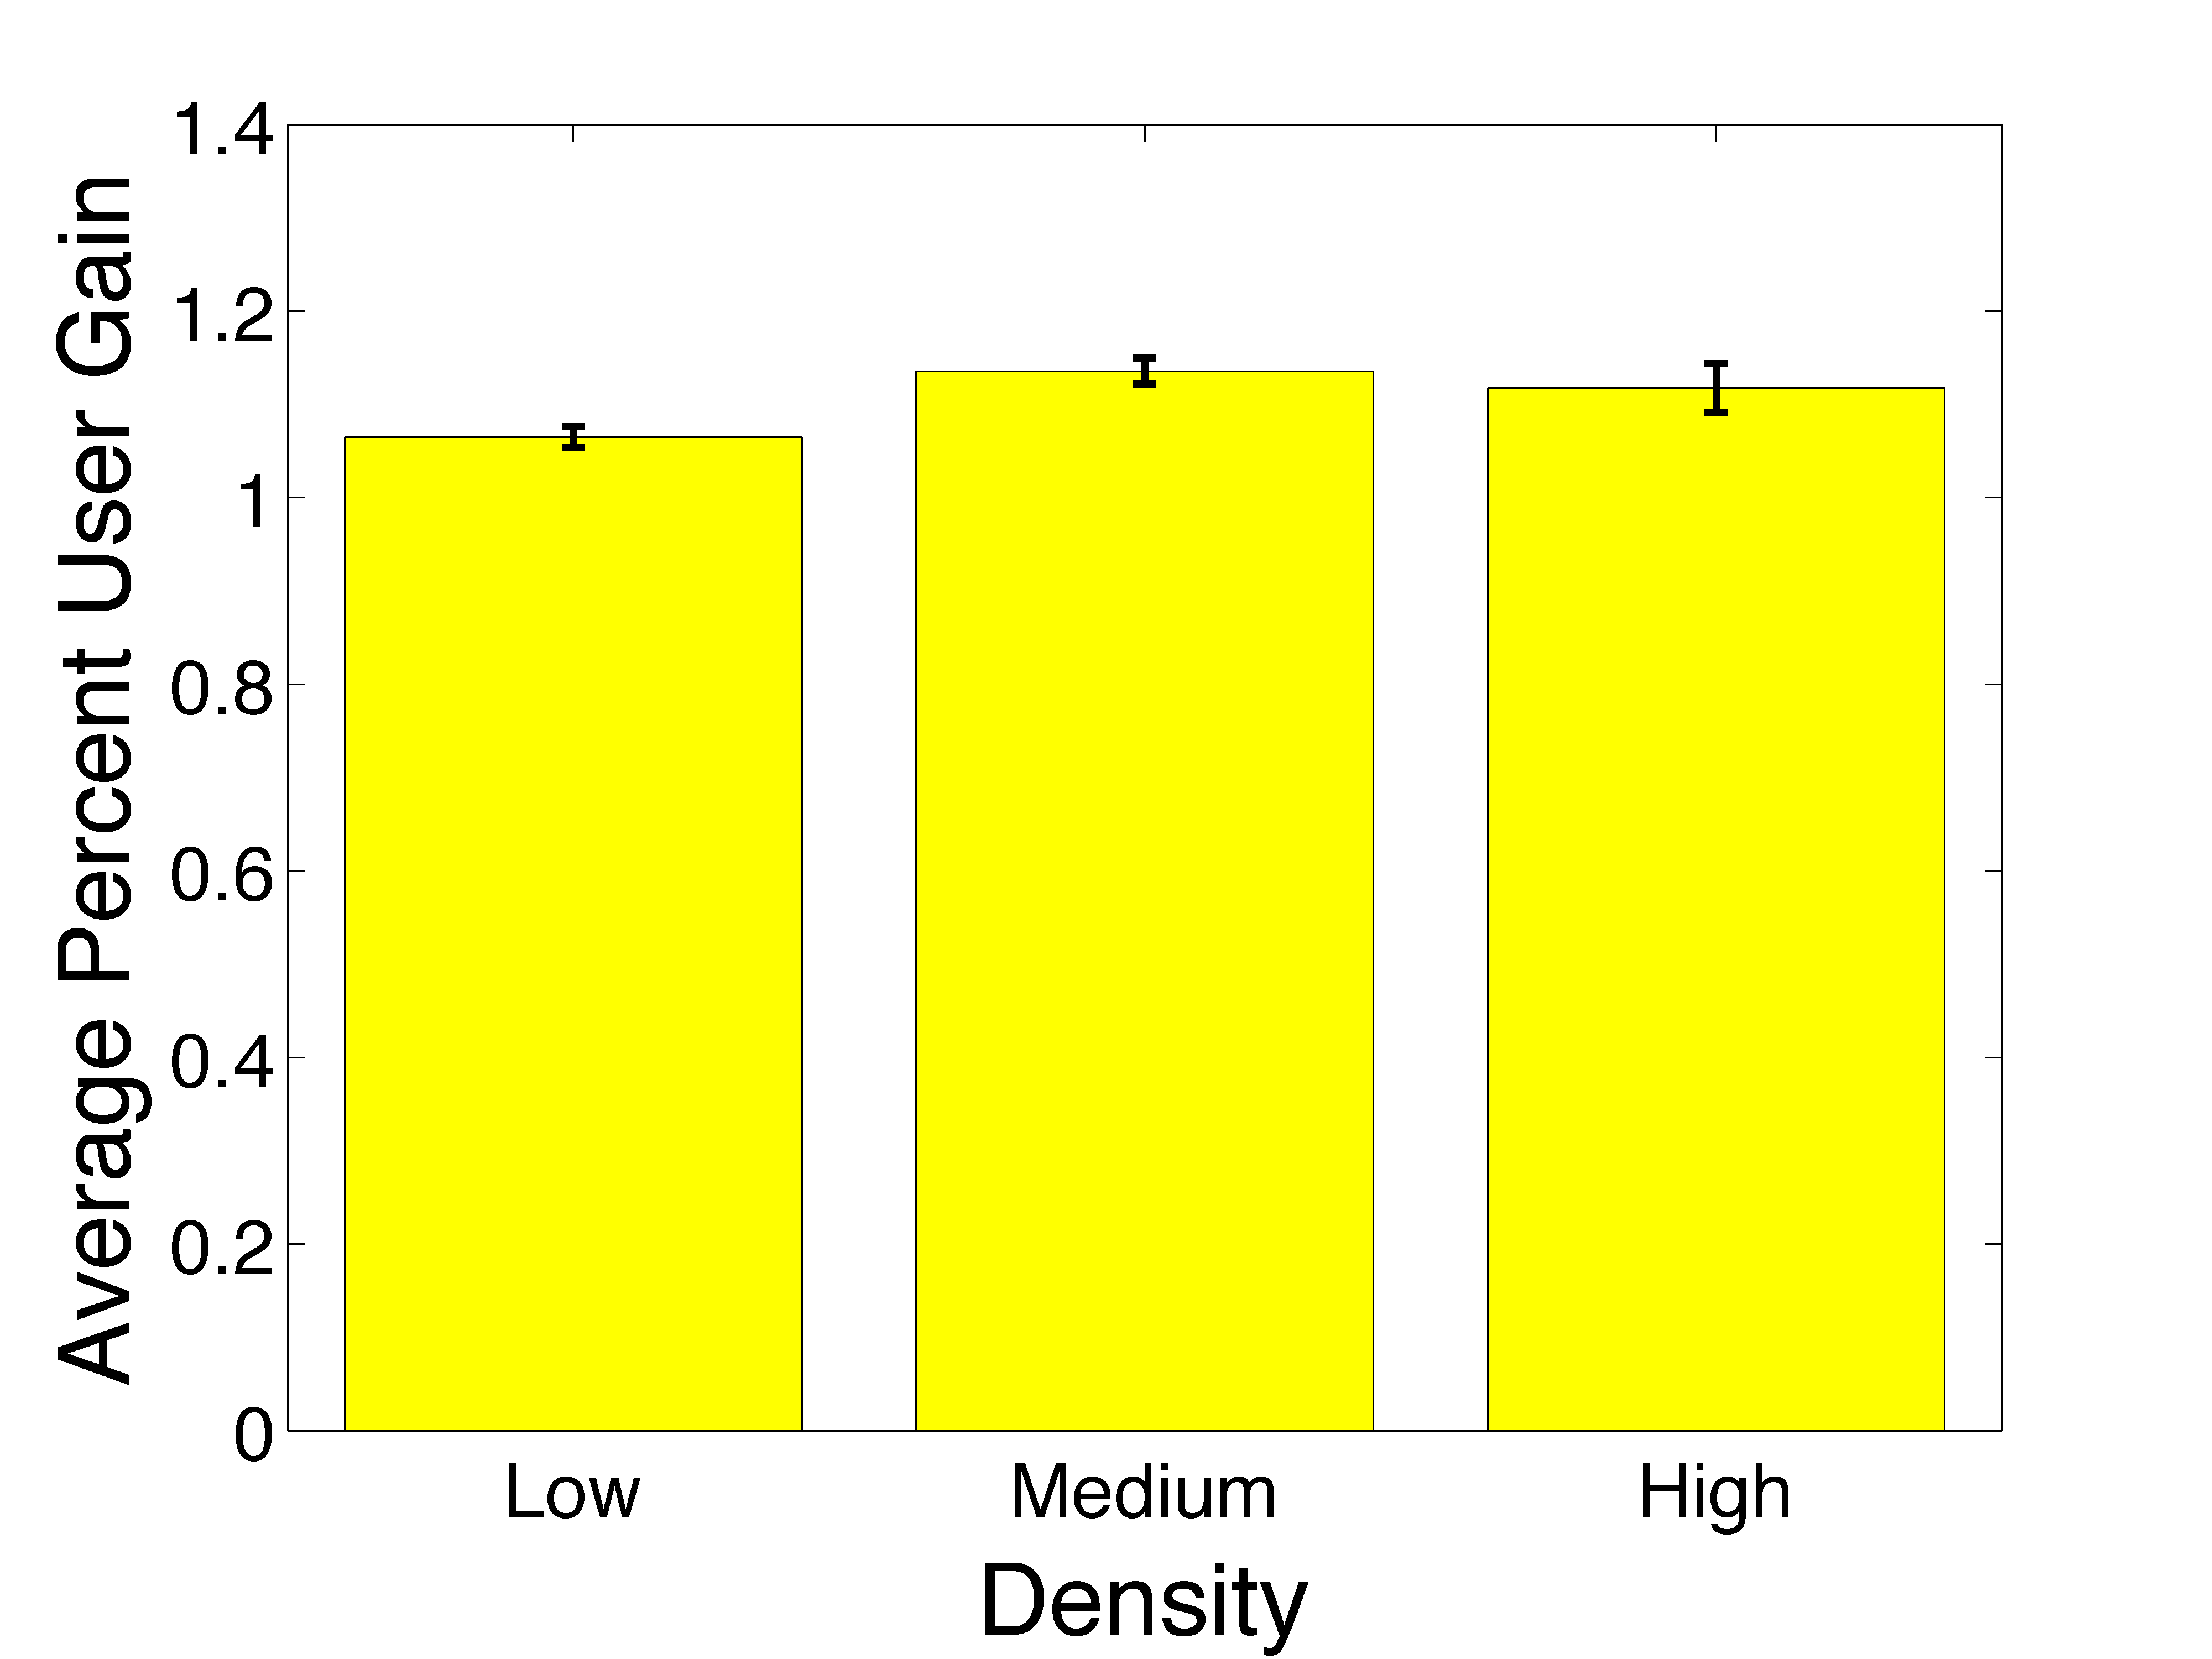
\includegraphics[width=0.33\textwidth,type=png,ext=.png,read=.png]{img/SmallWorld-0.875-AUG-PER}
	}    
   \hspace{-0.1in}\subfigure[Random Graphs M3.]{
	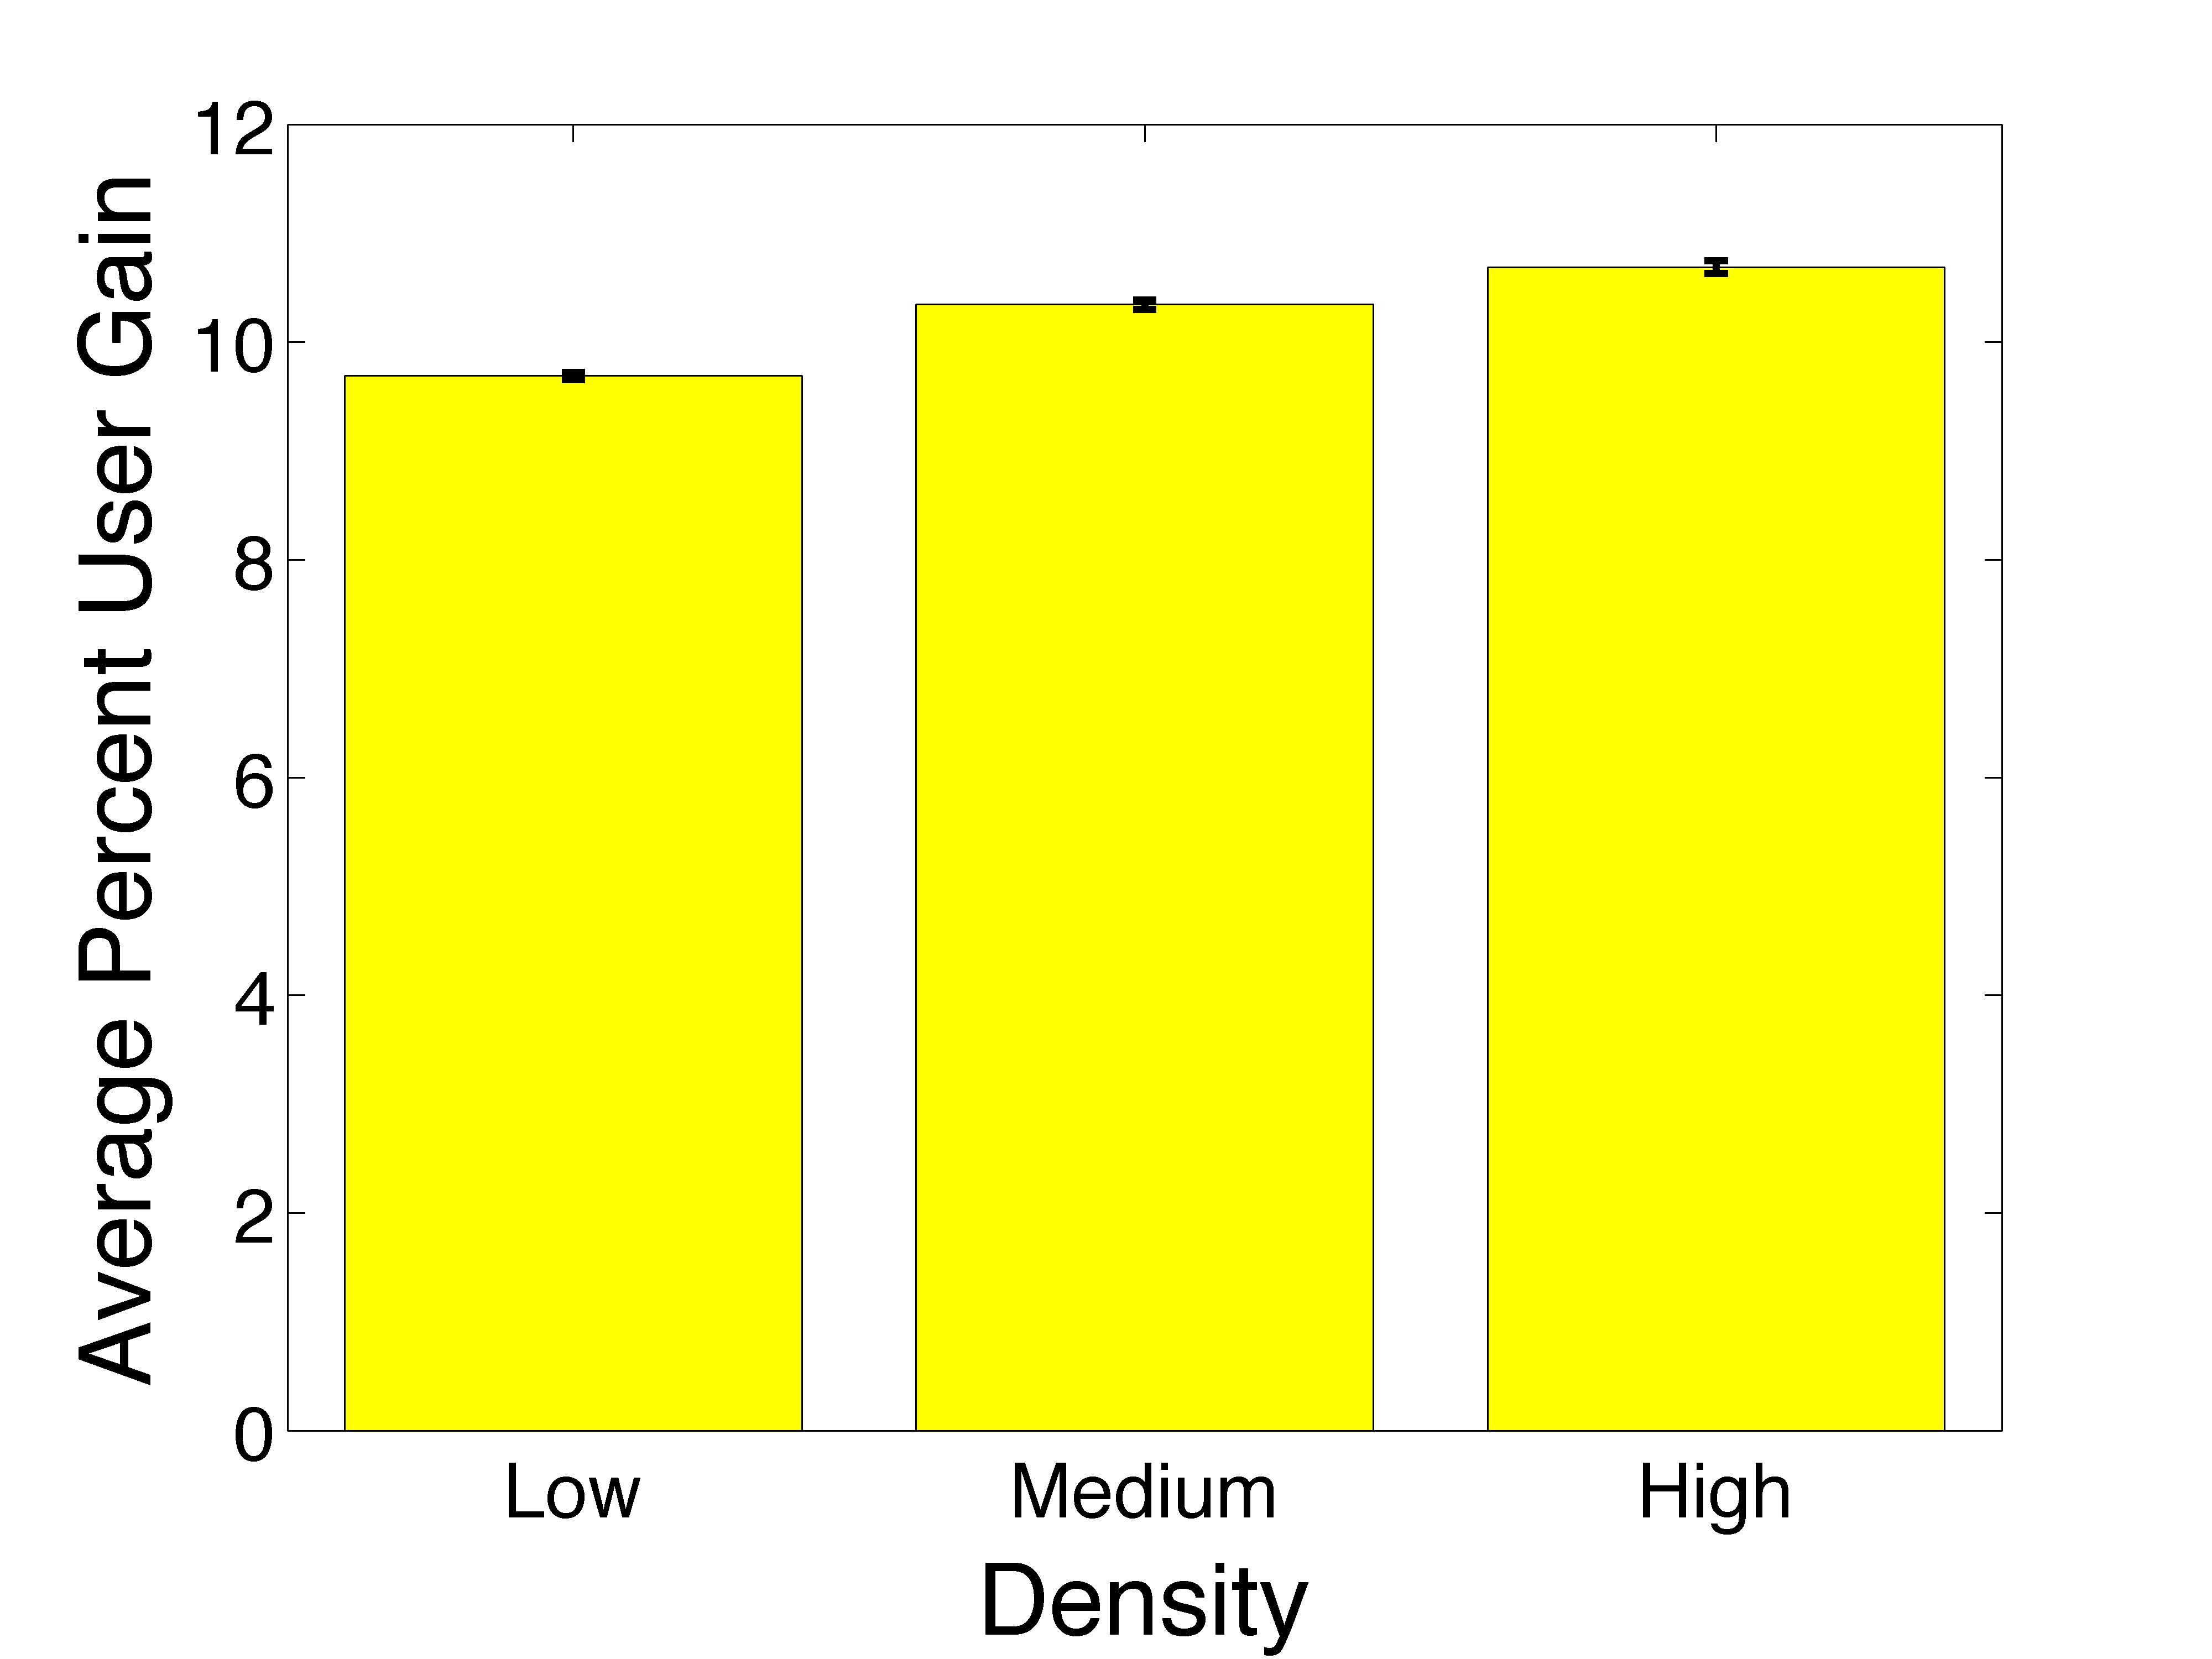
\includegraphics[width=0.33\textwidth,type=png,ext=.png,read=.png]{img/Random-0.500-AUG-PER}
	}  
  \hspace{-0.1in}\subfigure[Scale Free M3.]{
	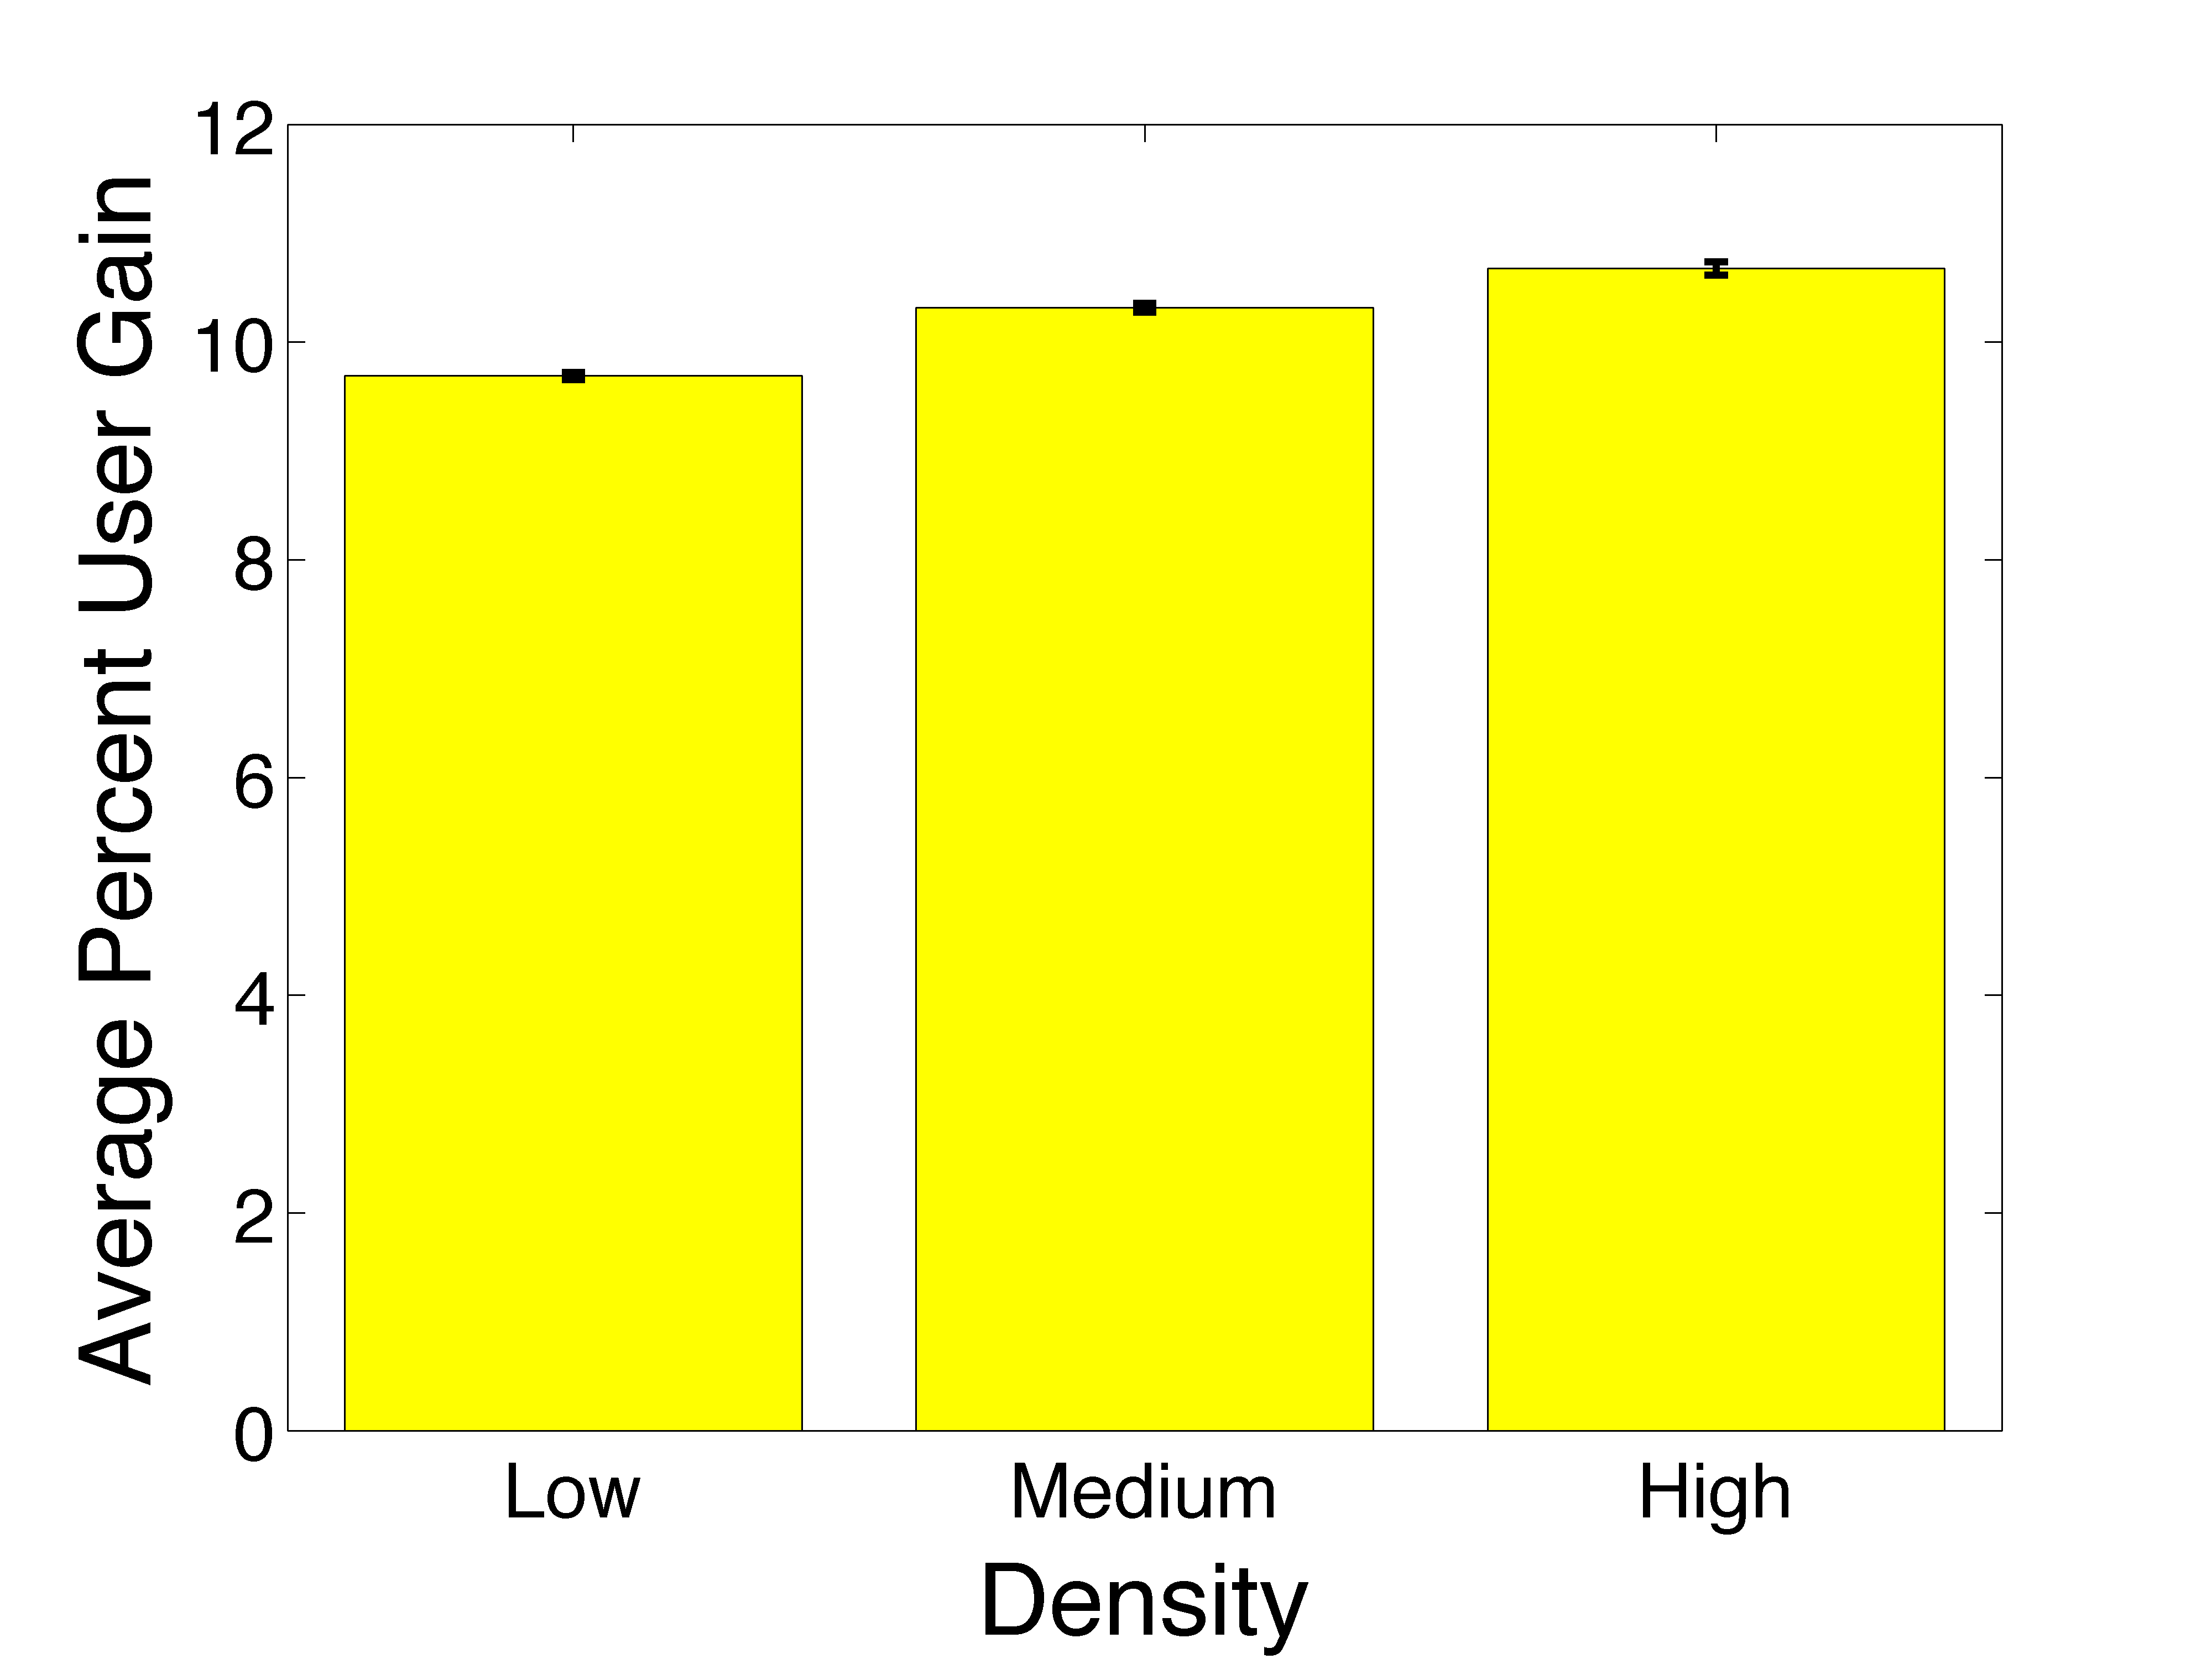
\includegraphics[width=0.33\textwidth,type=png,ext=.png,read=.png]{img/ScaleFree-0.500-AUG-PER}
	}  
  \hspace{-0.1in}\subfigure[Small World M3.]{
	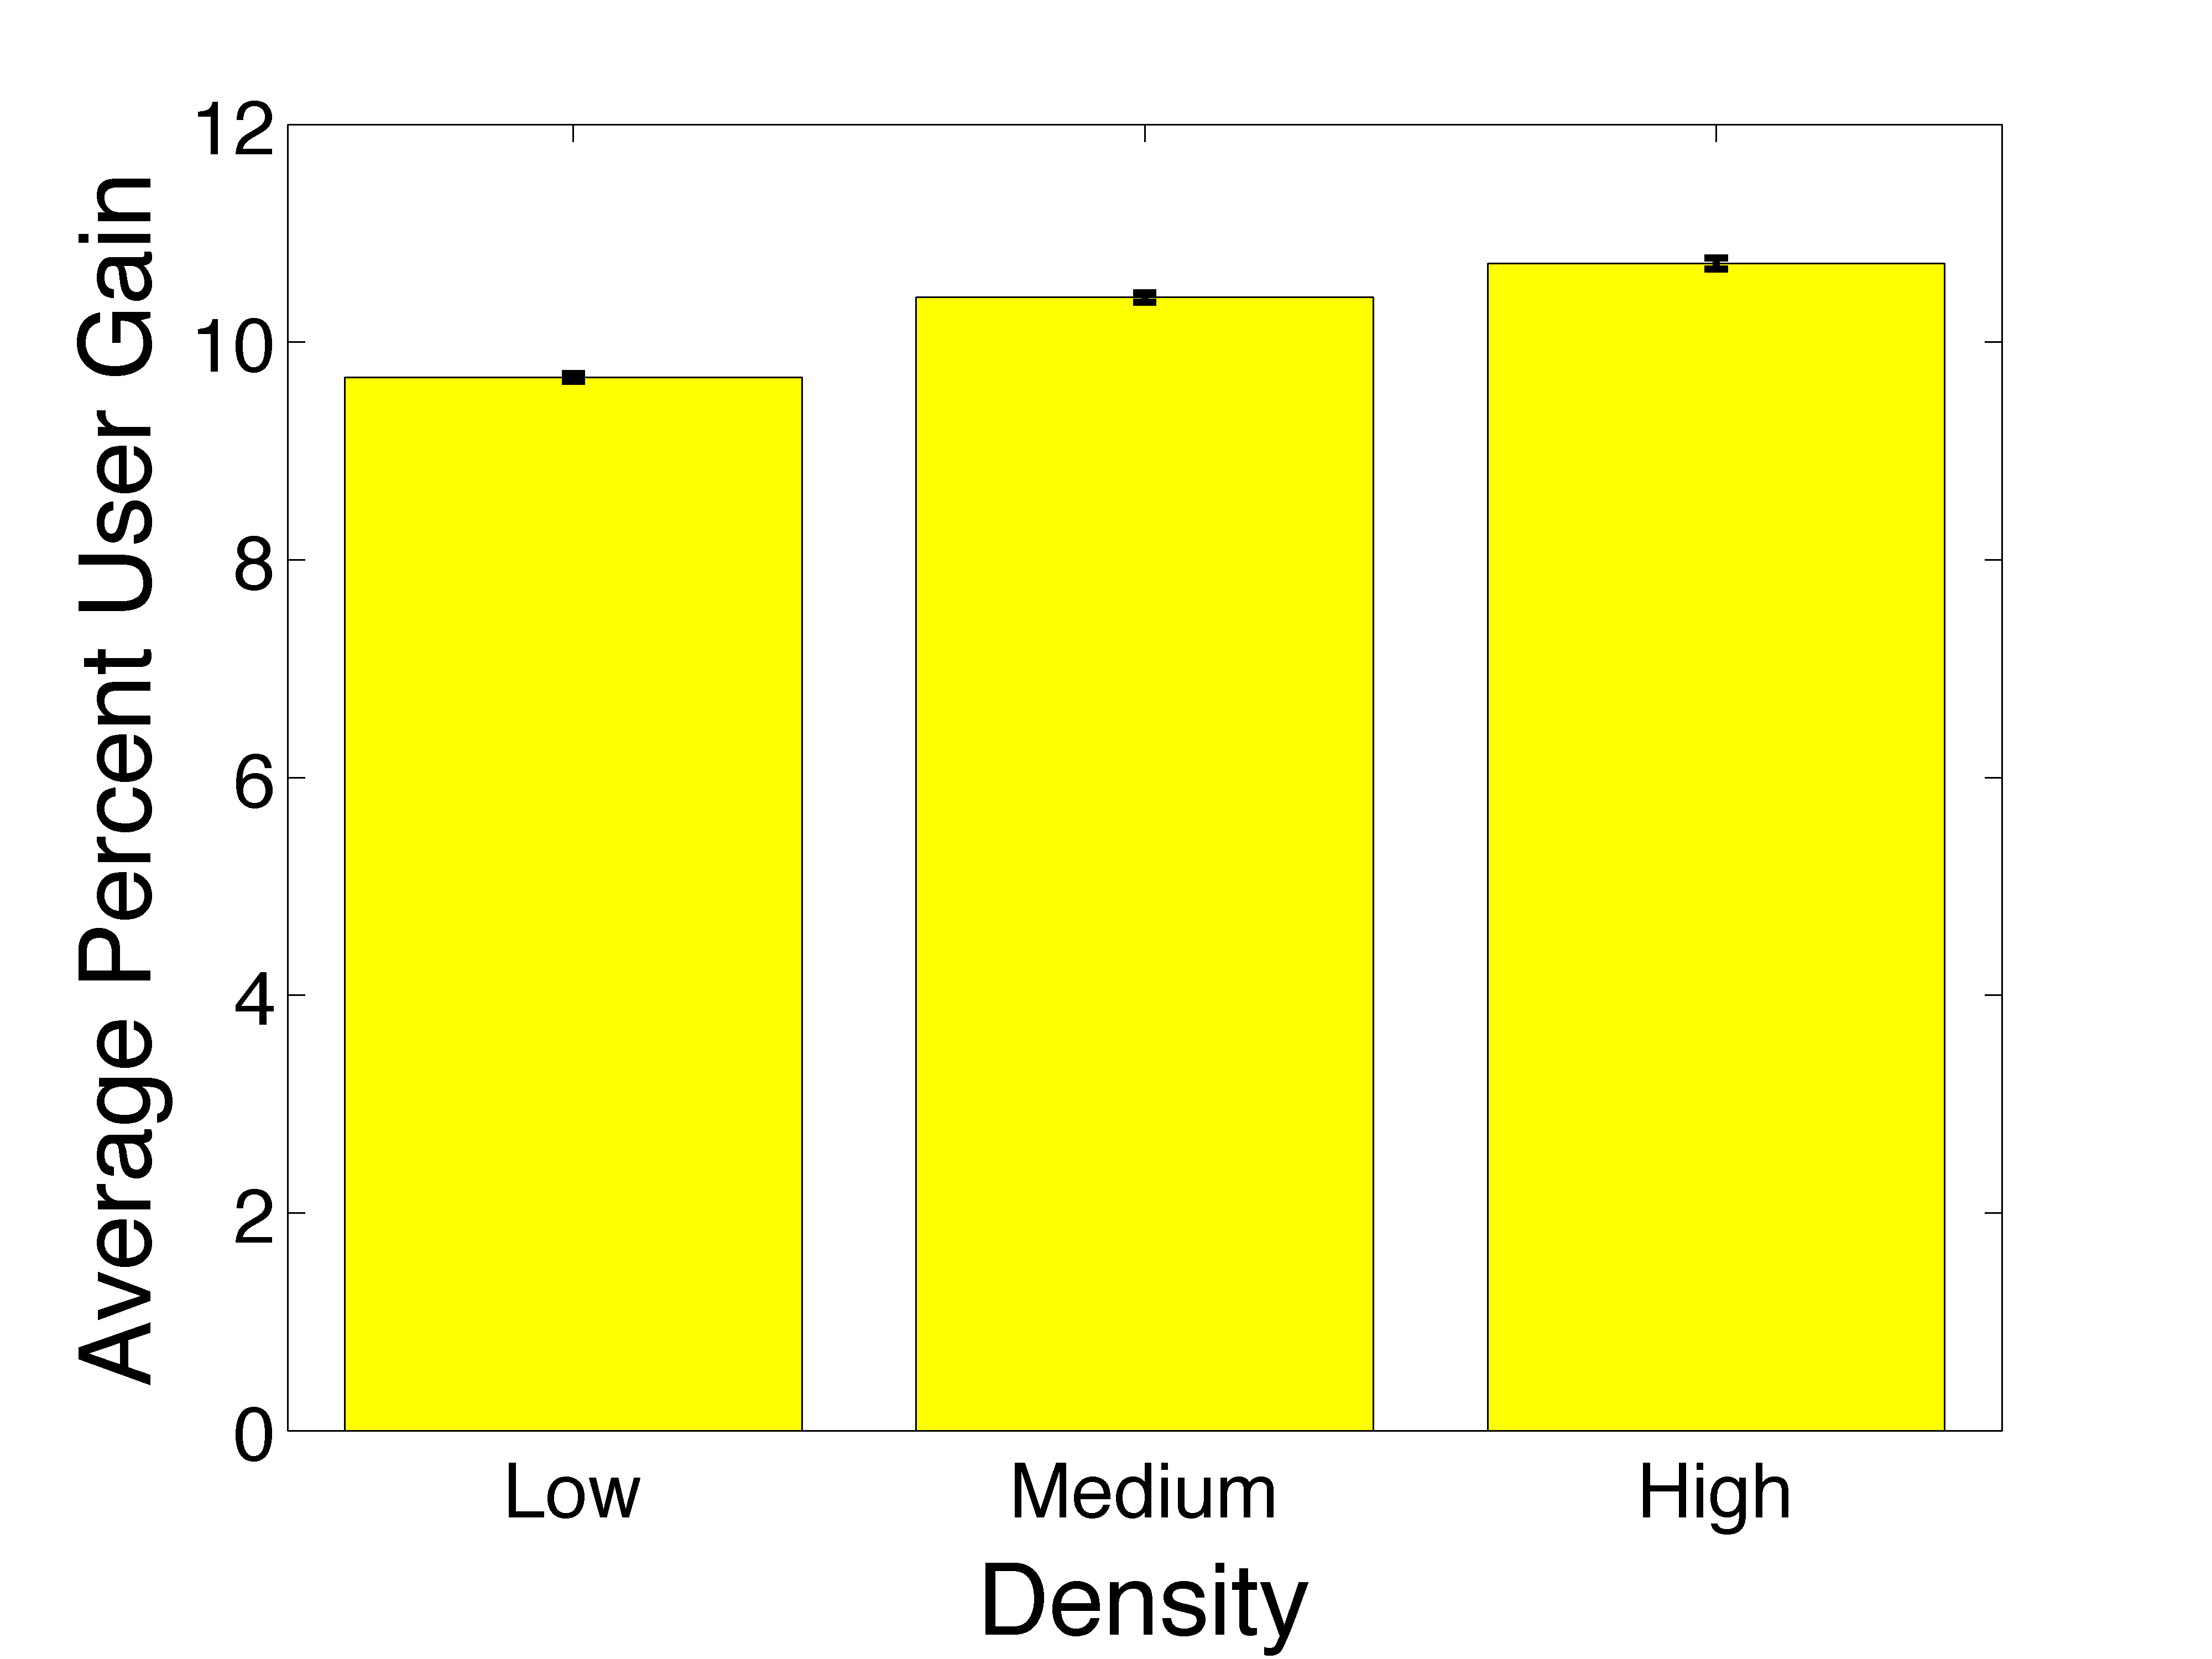
\includegraphics[width=0.33\textwidth,type=png,ext=.png,read=.png]{img/SmallWorld-0.500-AUG-PER}
	}   
  \caption{Graphs showing the average percent gain of consumers on
  different topologies and densities under market conditions M1 (a)-(c), M2
  (d)-(f) and M3 (g)-(i).
  }
  \label{fig:graphs_gain}
\end{figure*}



% \begin{figure*}  
%   \centering  
%   \hspace{-0.1in}\subfigure[Random Graphs.]{
% 	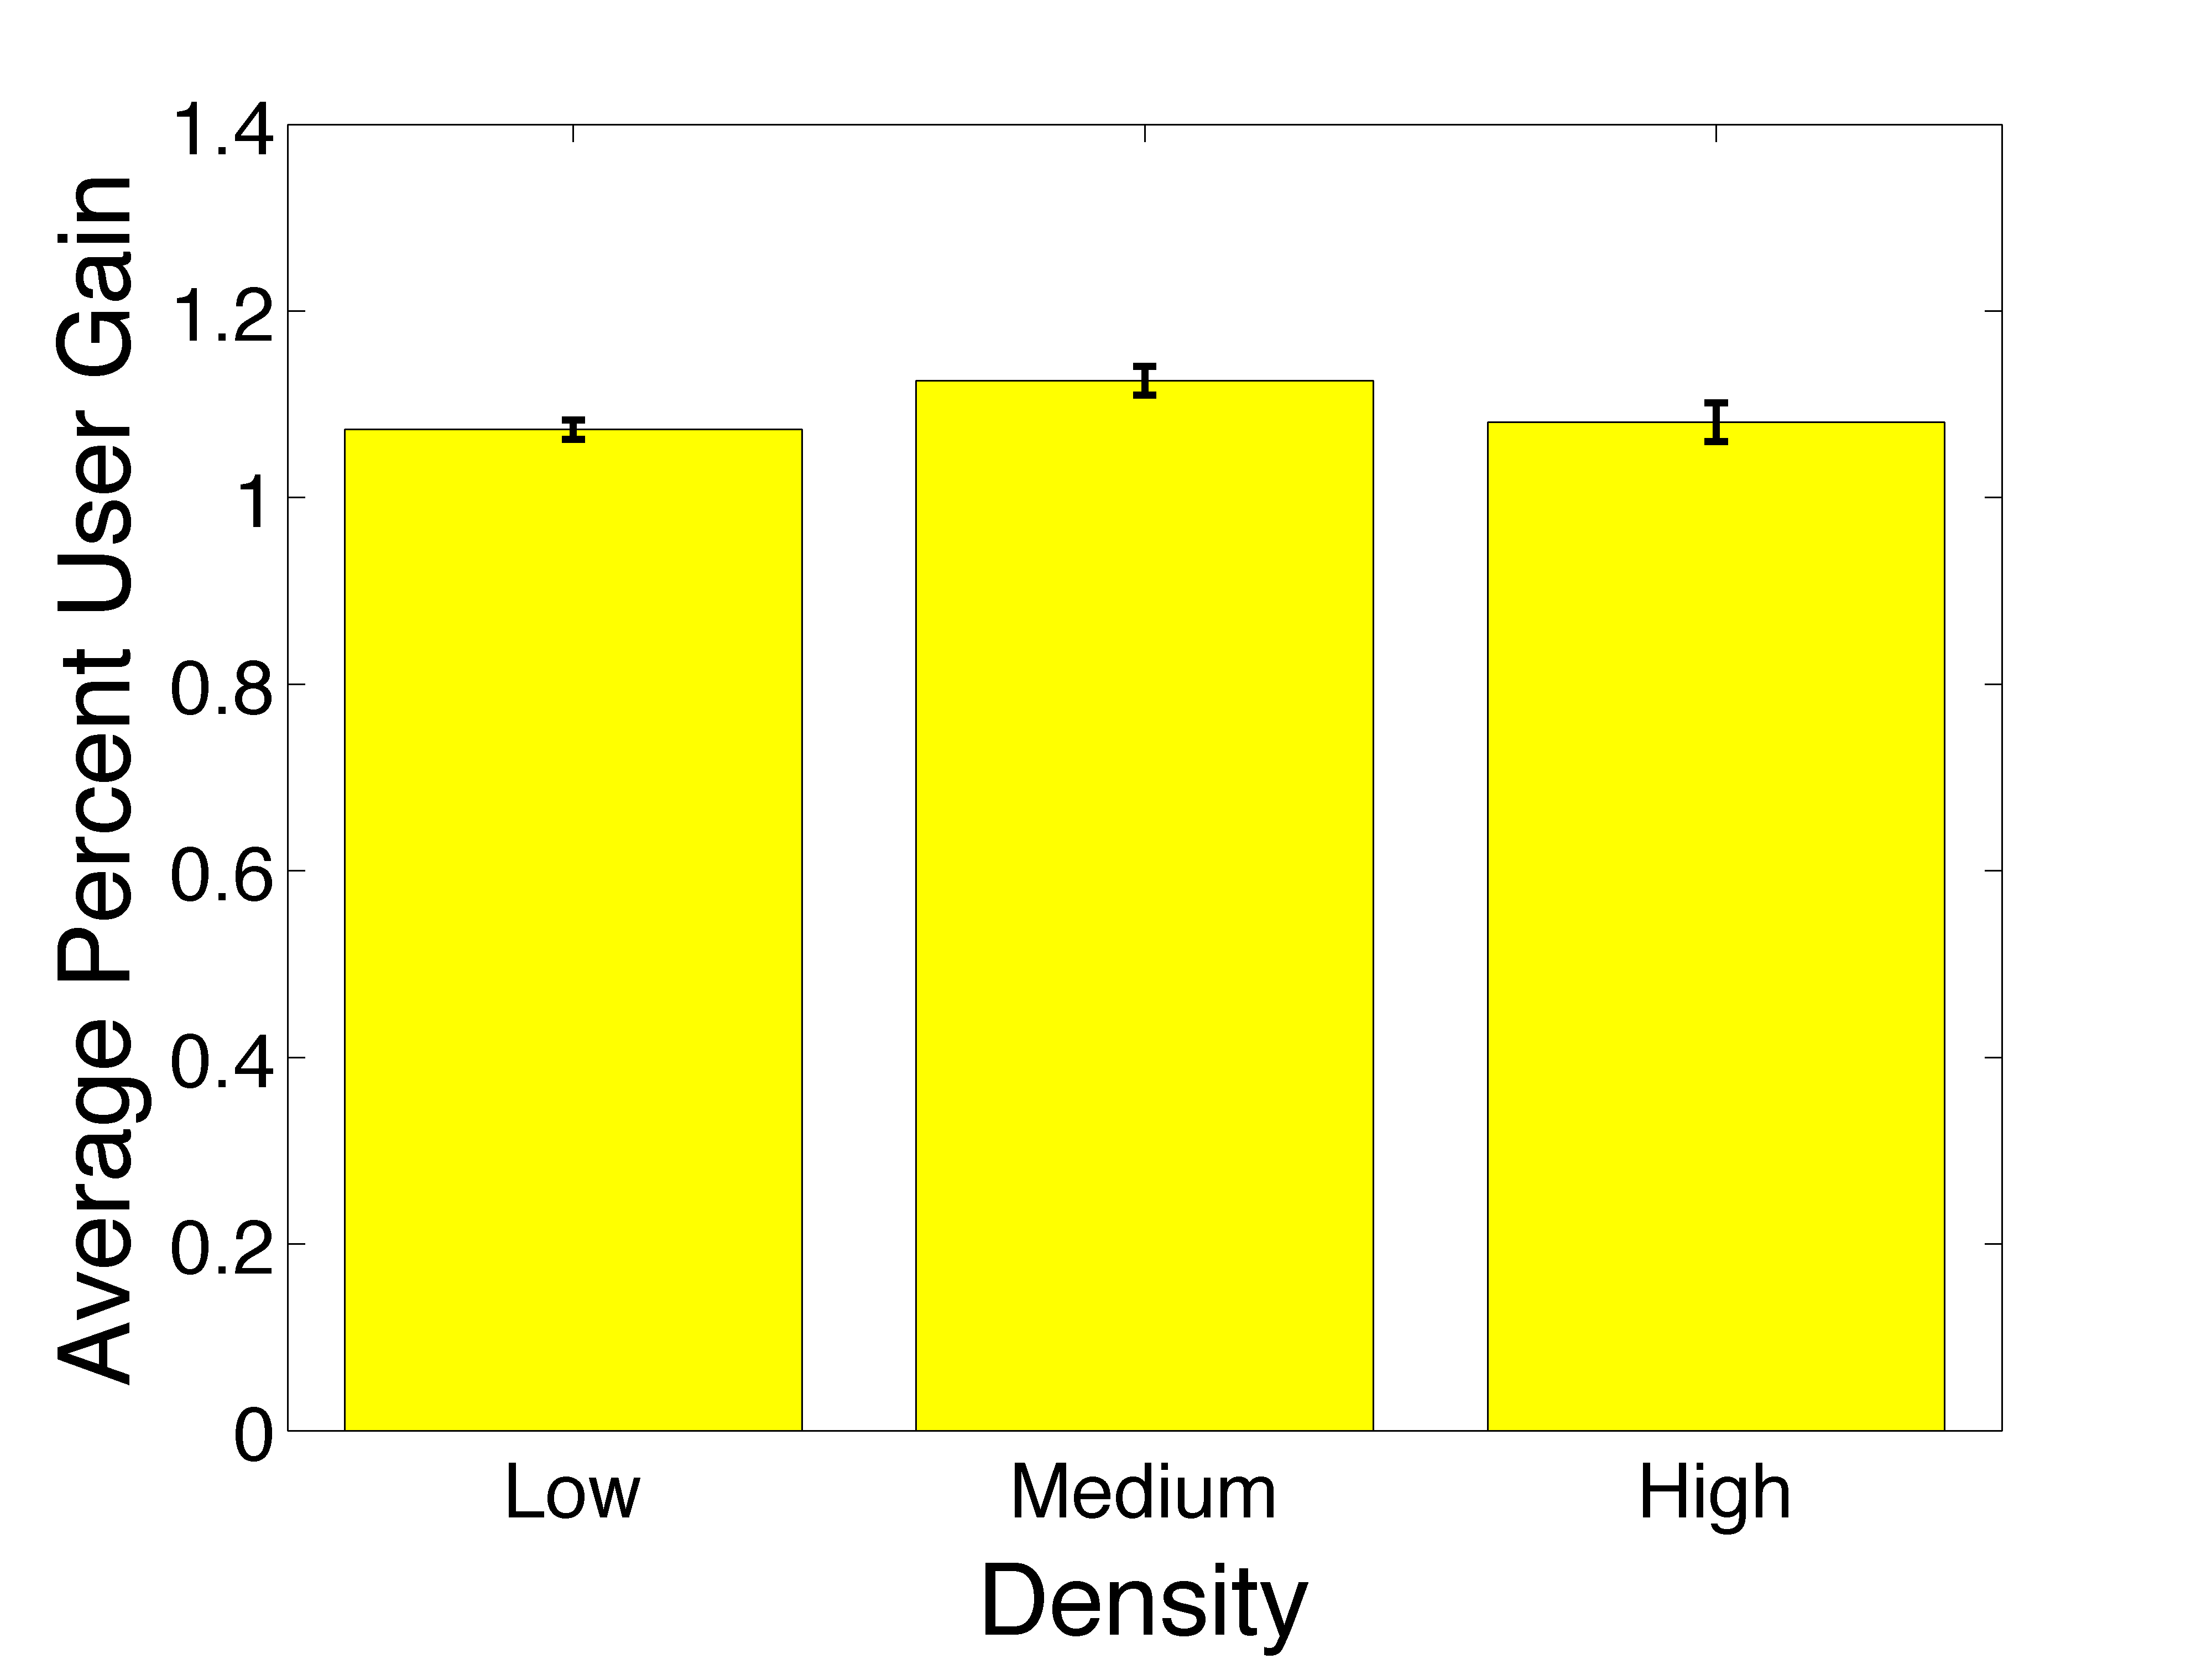
\includegraphics[width=0.33\textwidth,type=png,ext=.png,read=.png]{img/Random-0.875-AUG-PER}
% 	}  
%   \hspace{-0.1in}\subfigure[Scale Free.]{
% 	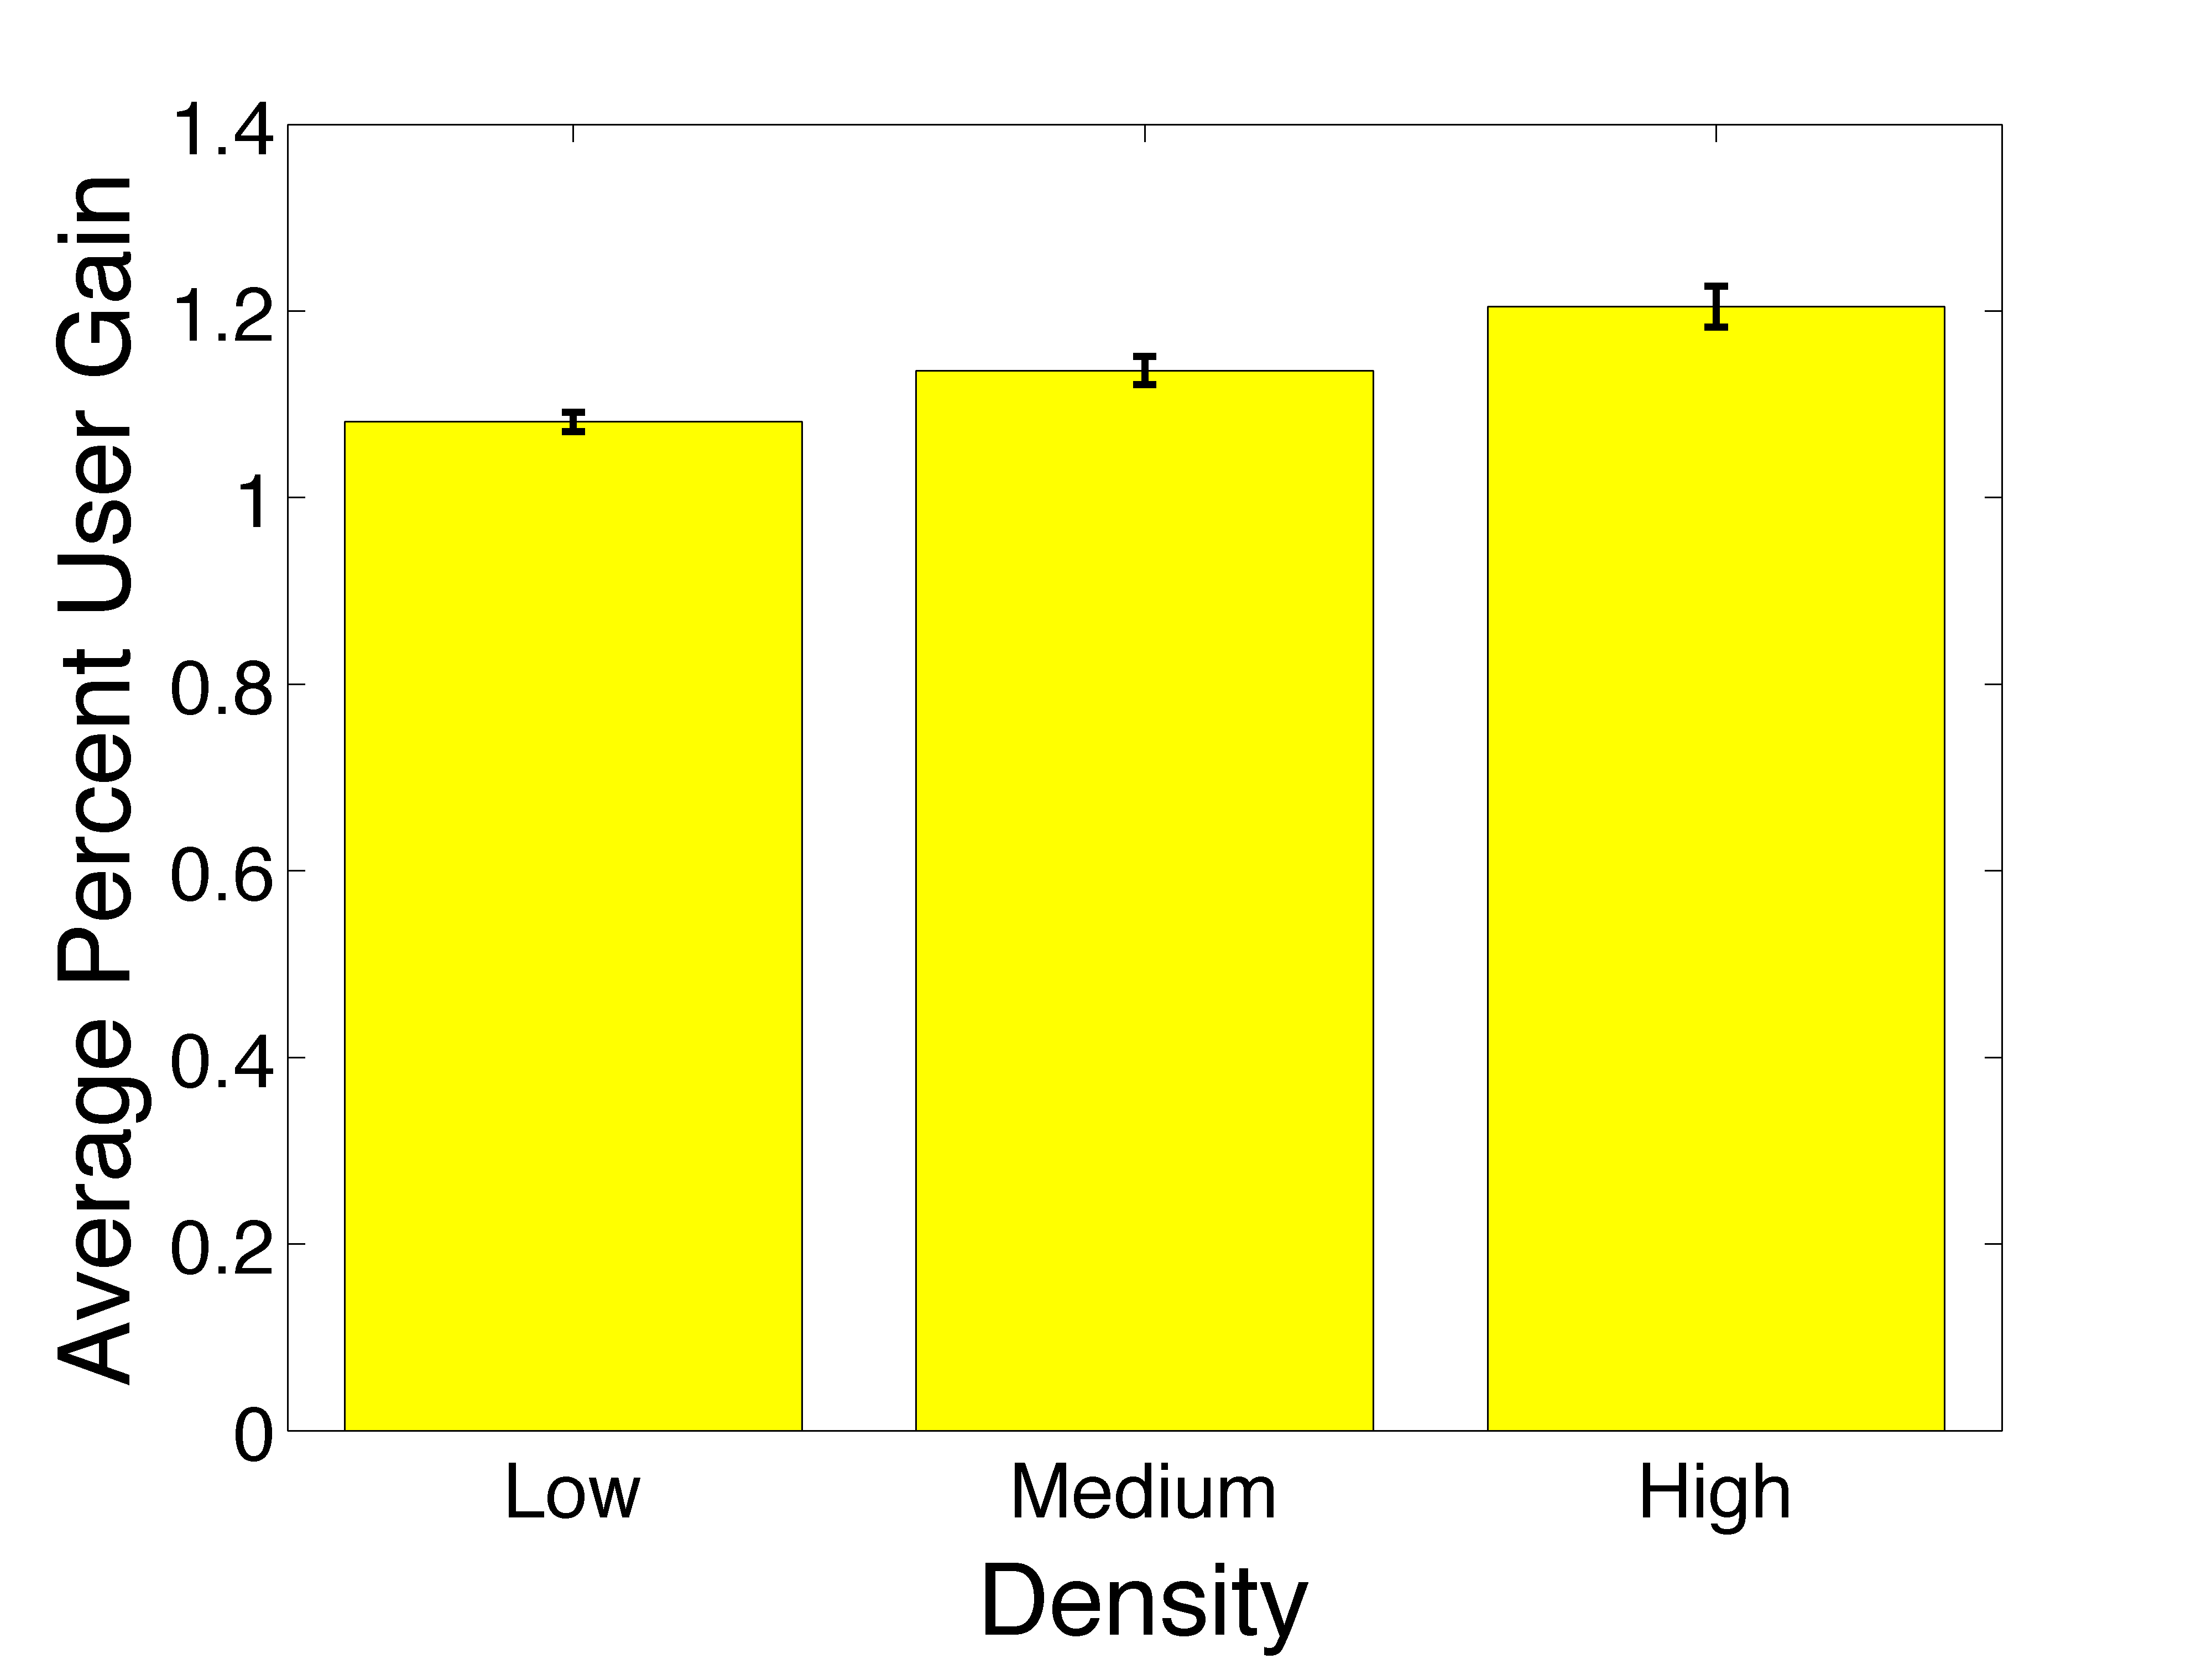
\includegraphics[width=0.33\textwidth,type=png,ext=.png,read=.png]{img/ScaleFree-0.875-AUG-PER}
% 	}  
%   \hspace{-0.1in}\subfigure[Small World.]{
%   	%\label{fig:res_mmuca_time}
% 	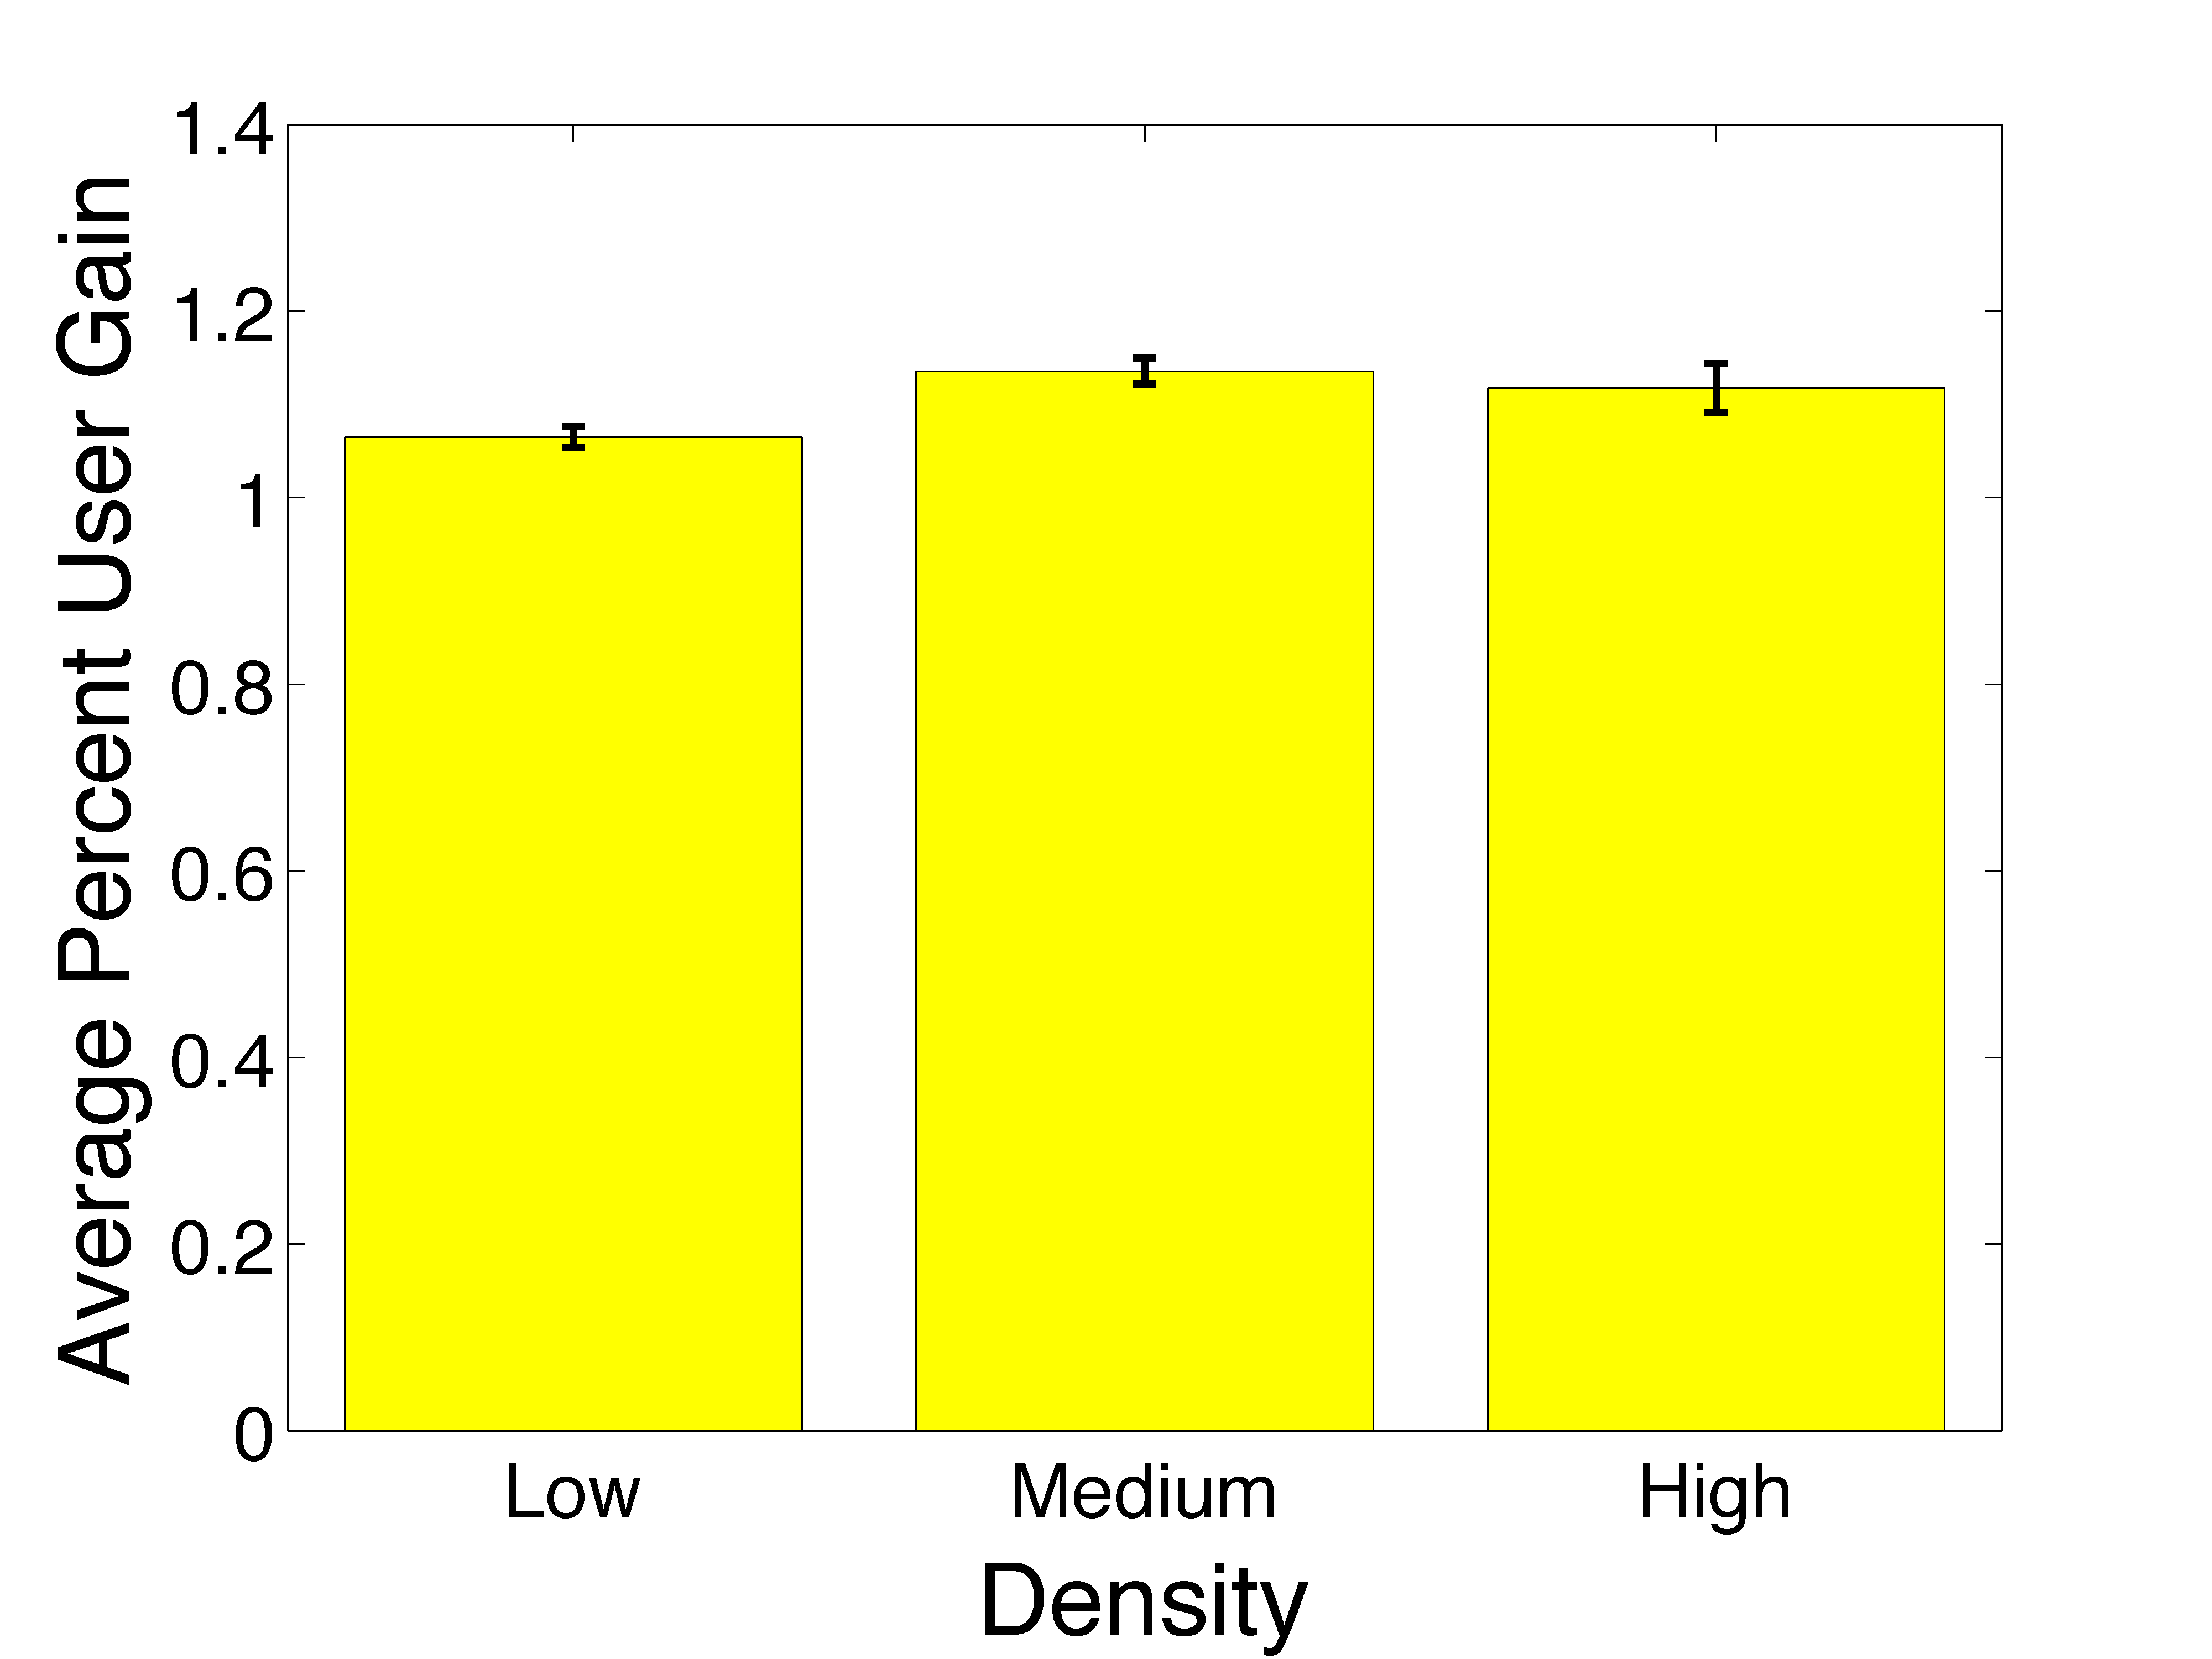
\includegraphics[width=0.33\textwidth,type=png,ext=.png,read=.png]{img/SmallWorld-0.875-AUG-PER}
% 	}    
%   \caption{$70/80 p=0.875$ Graphs showing the average percent gain of consumers'
%   payoffs in the coalitions with respect to the payoff of individual coalitions on
%   different topologies and with different densities. }
%   \label{fig:graphs_gain}
% \end{figure*}

% \begin{figure*}  
%   \centering  
%   \hspace{-0.1in}\subfigure[Random Graphs.]{
% 	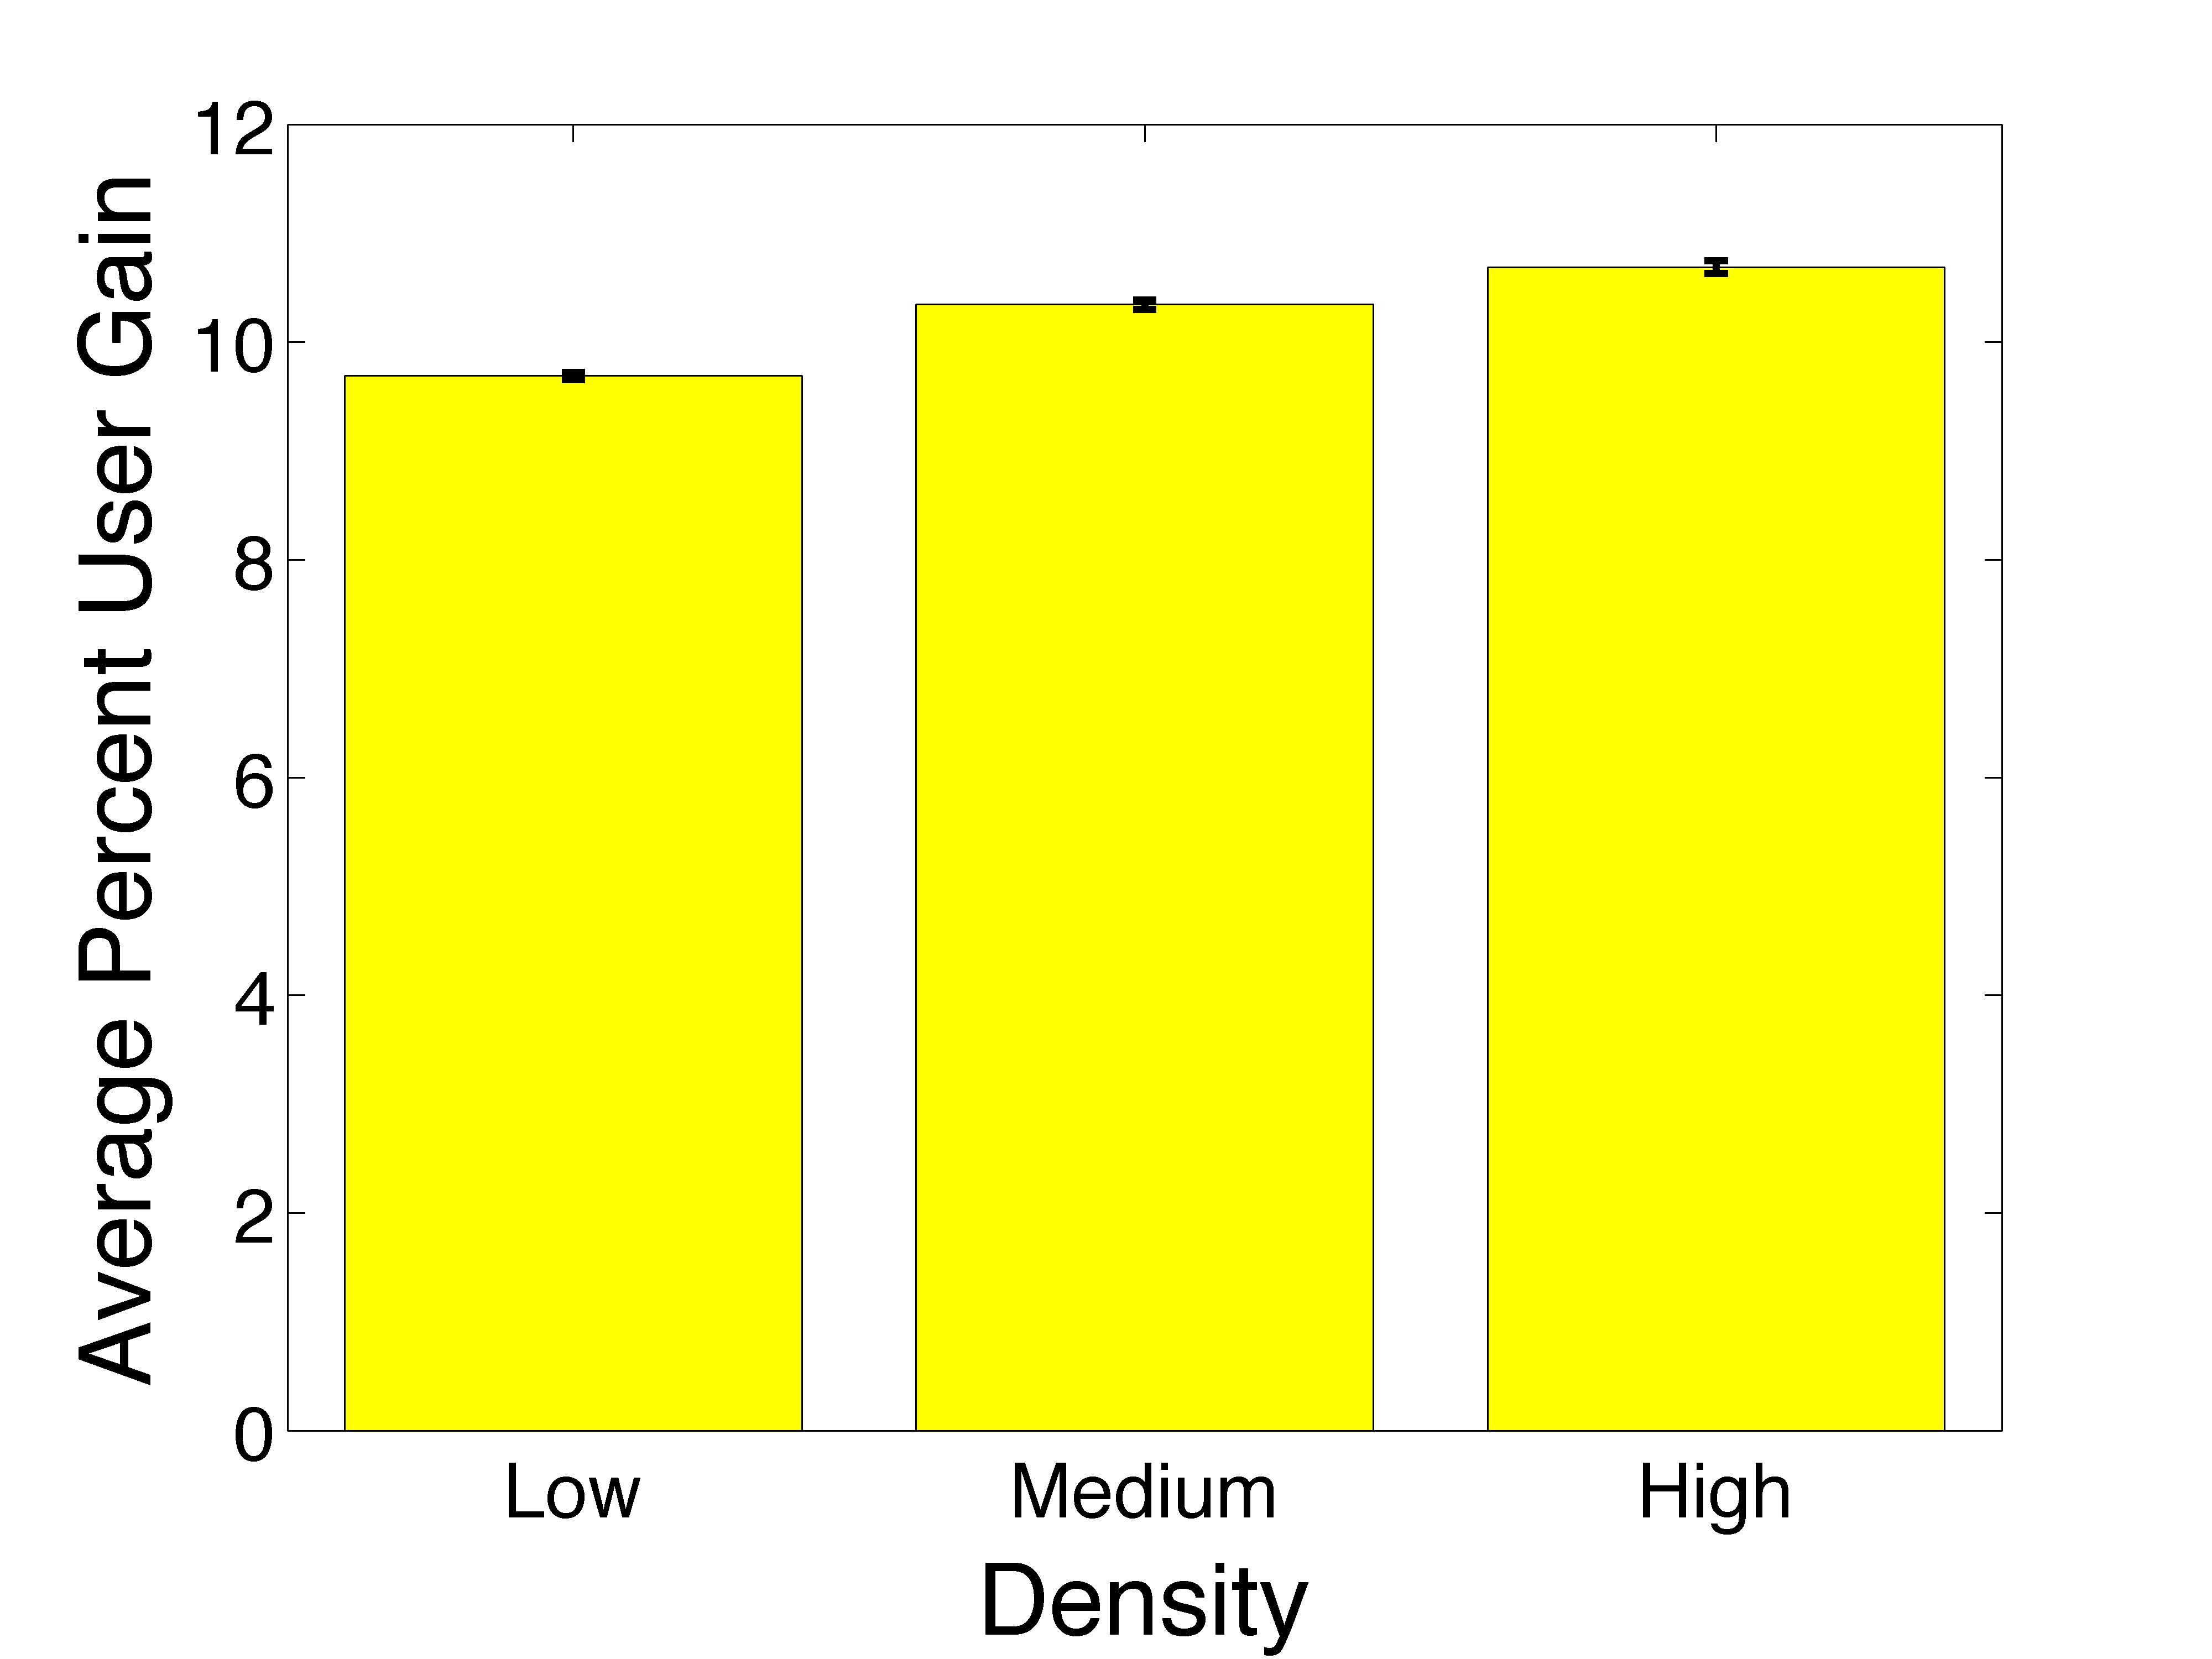
\includegraphics[width=0.33\textwidth,type=png,ext=.png,read=.png]{img/Random-0.500-AUG-PER}
% 	}  
%   \hspace{-0.1in}\subfigure[Scale Free.]{
% 	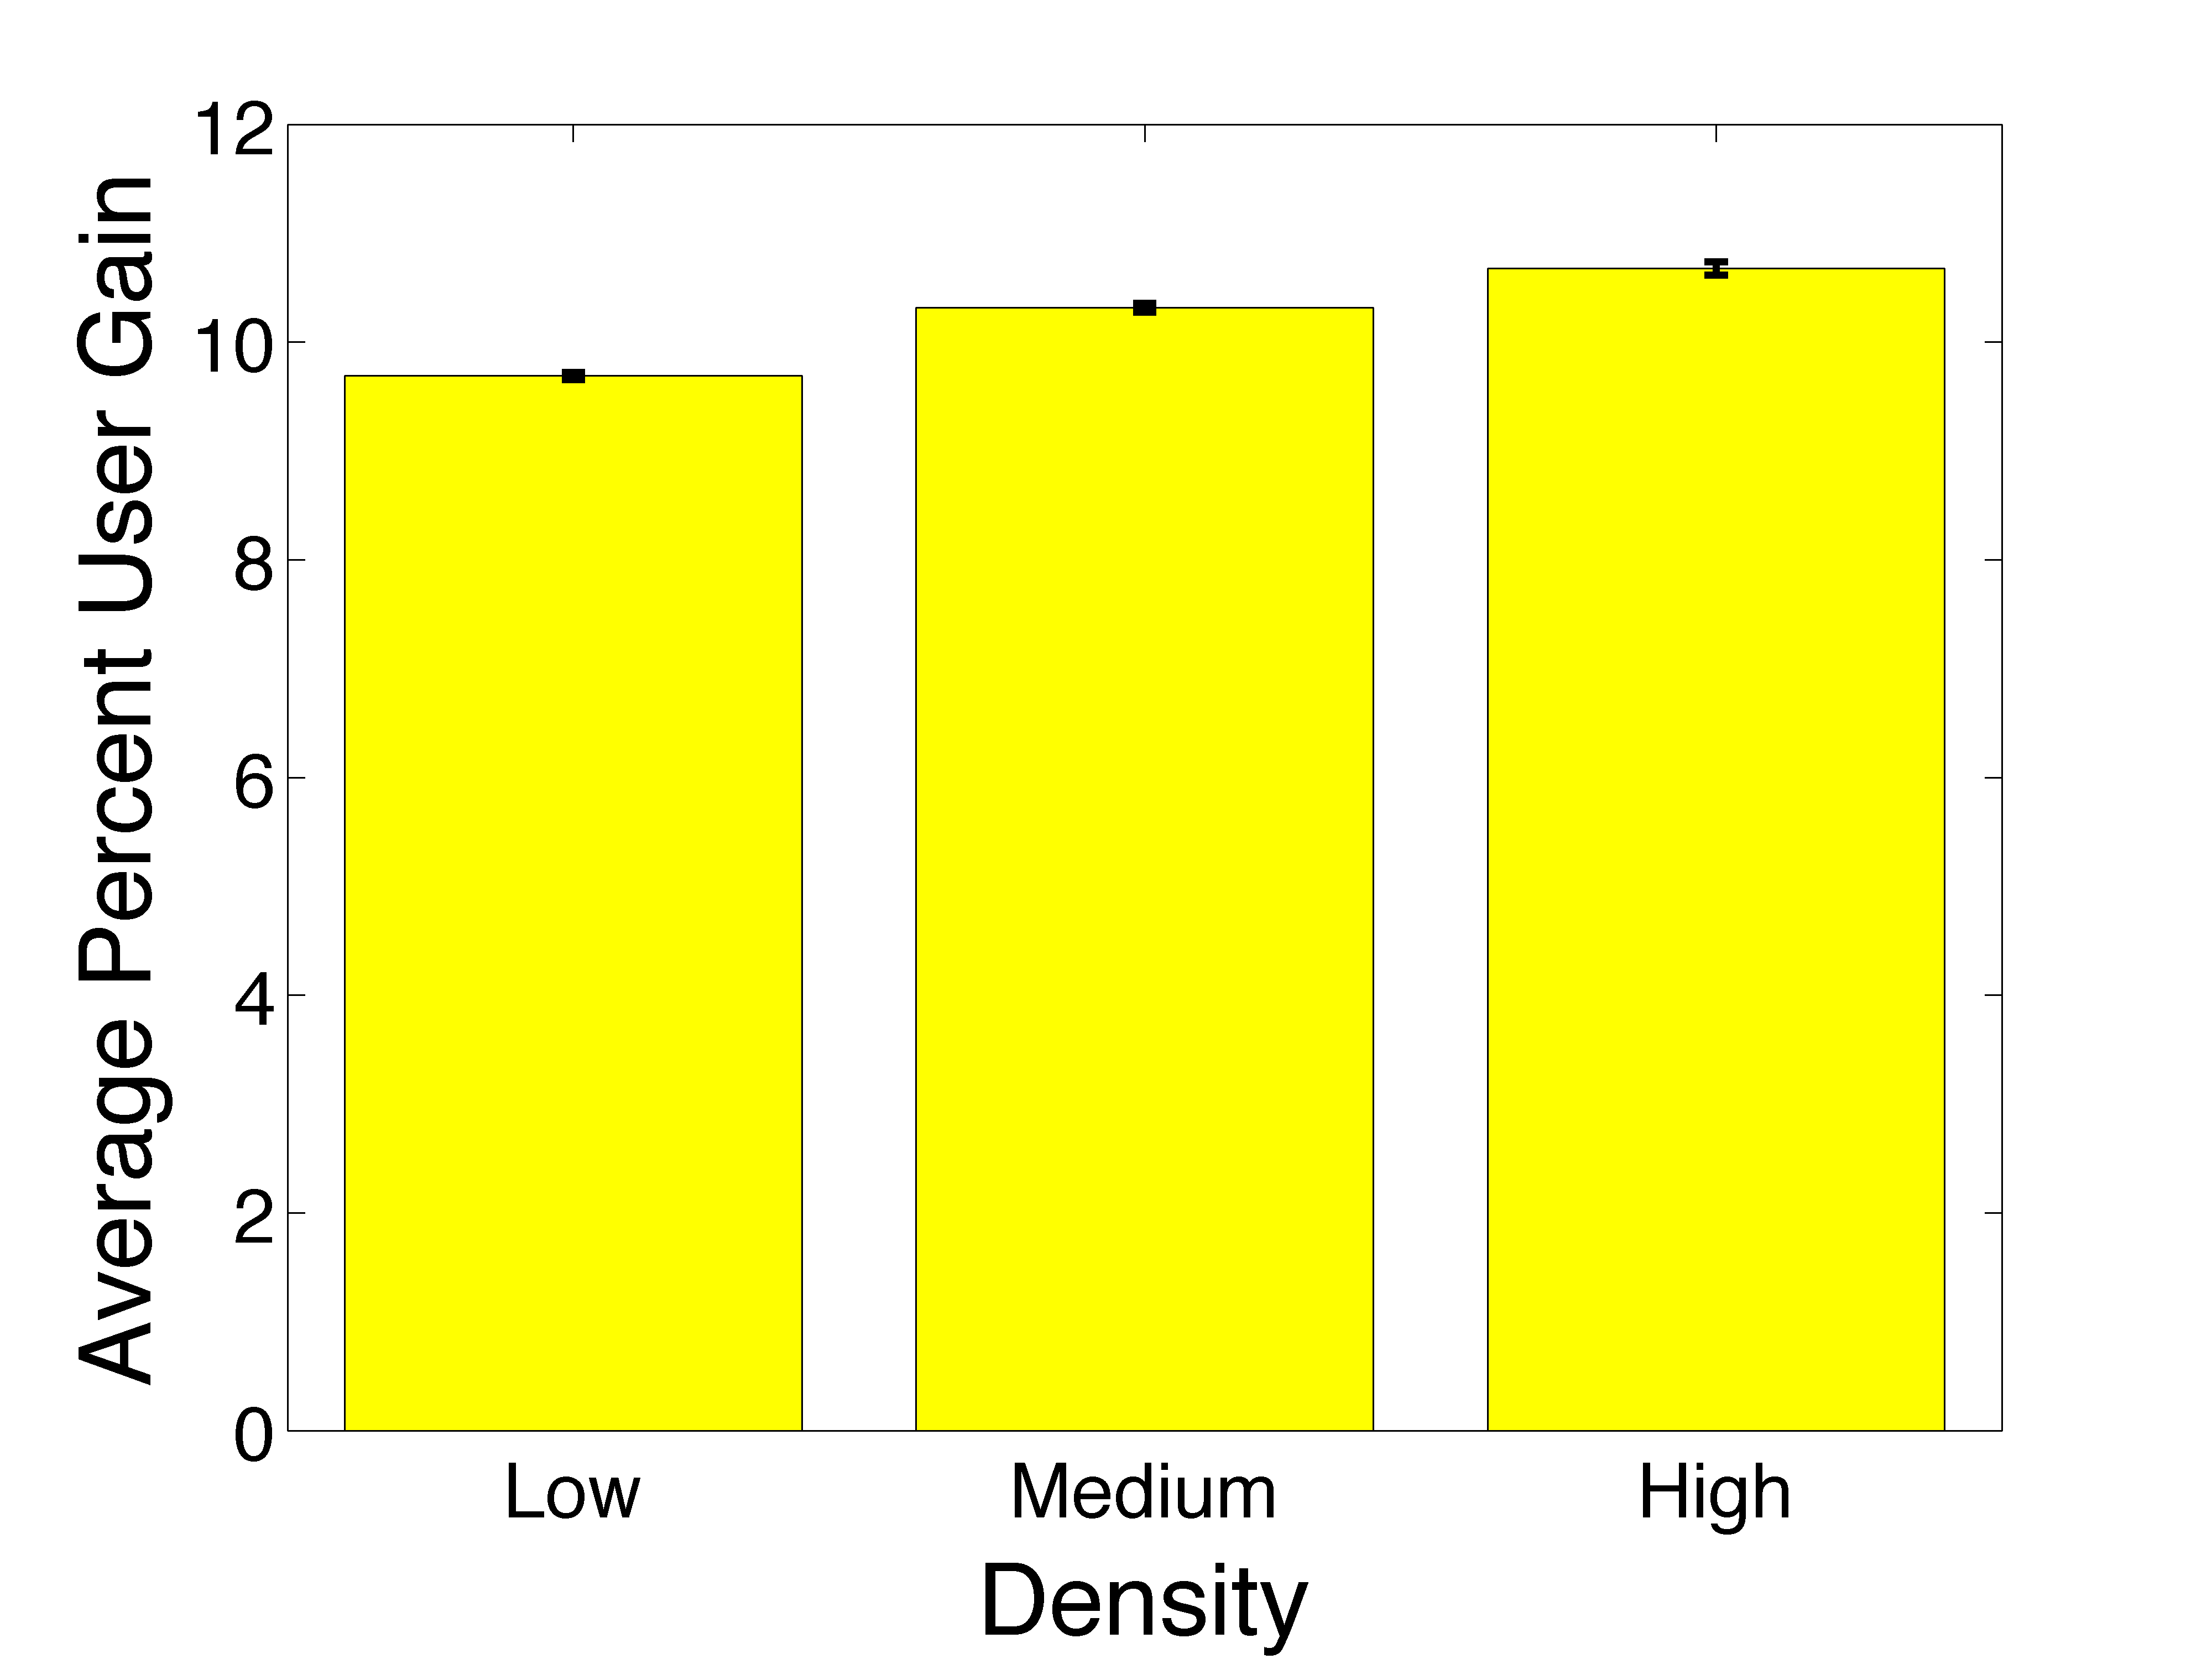
\includegraphics[width=0.33\textwidth,type=png,ext=.png,read=.png]{img/ScaleFree-0.500-AUG-PER}
% 	}  
%   \hspace{-0.1in}\subfigure[Small World.]{
%   	%\label{fig:res_mmuca_time}
% 	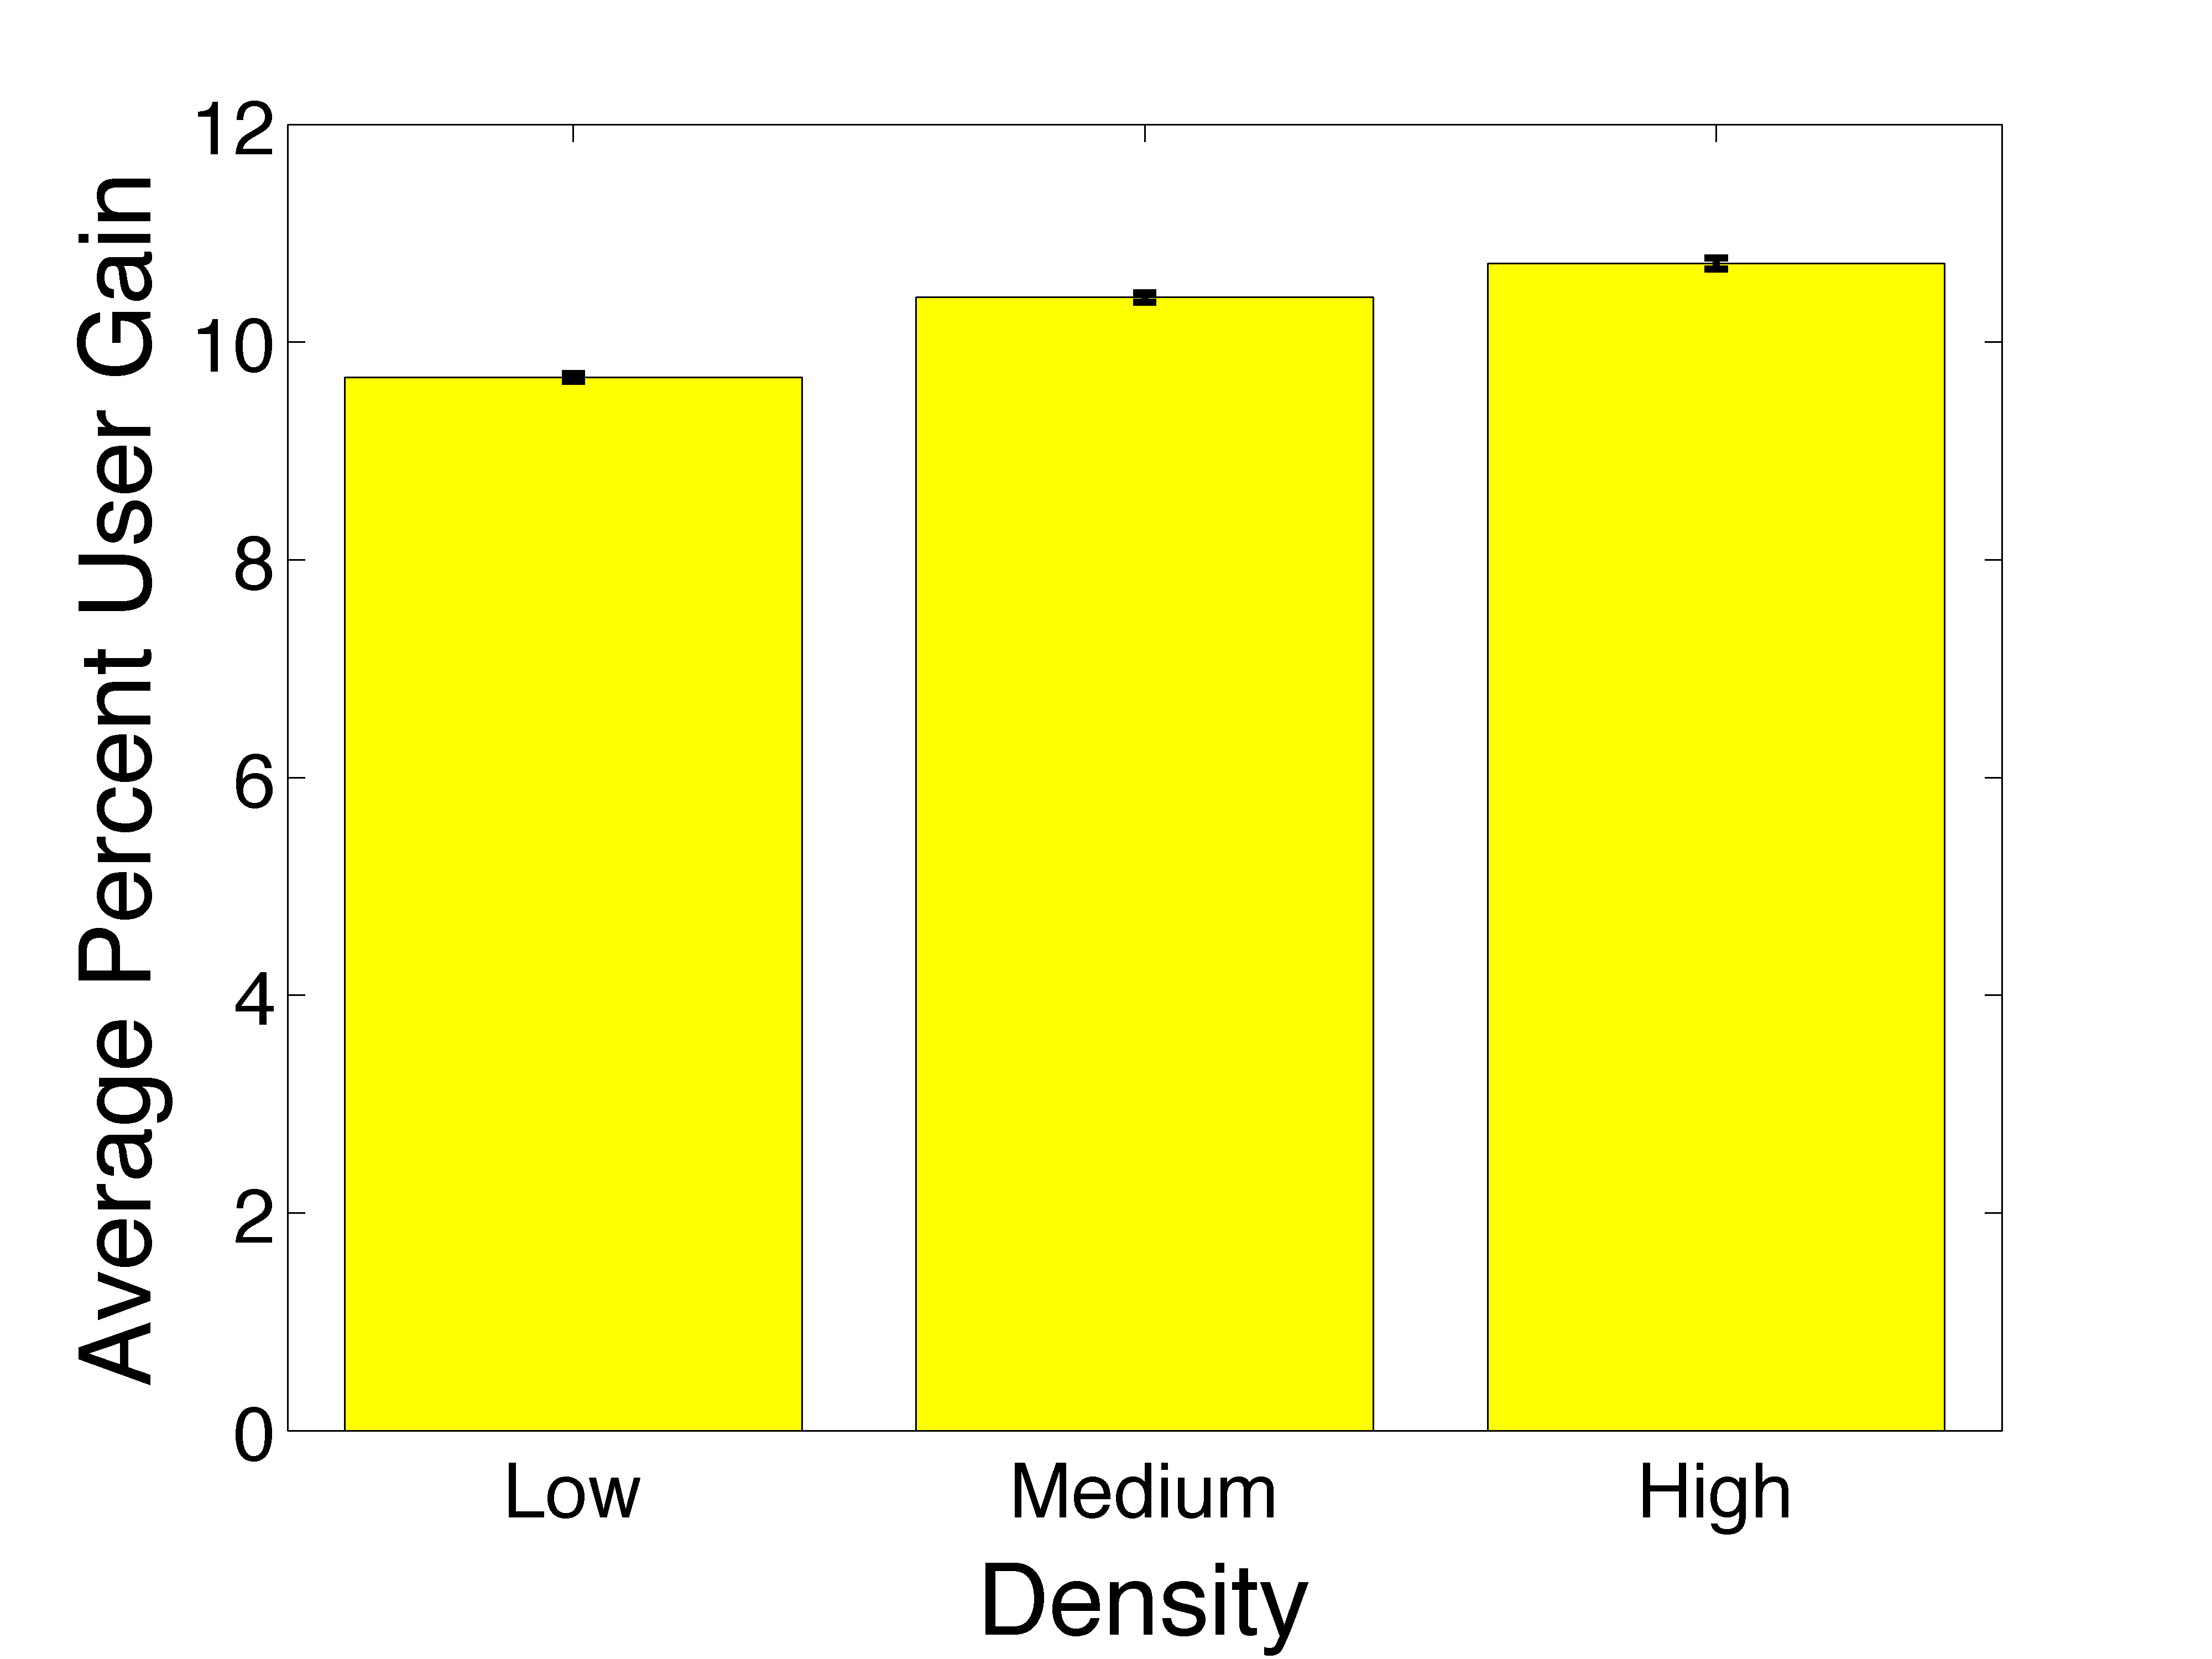
\includegraphics[width=0.33\textwidth,type=png,ext=.png,read=.png]{img/SmallWorld-0.500-AUG-PER}
% 	}    
%   \caption{$ p=0.500$ Graphs showing the average percent gain of consumers'
%   payoffs in the coalitions with respect to the payoff of individual coalitions on
%   different topologies and with different densities. }
%   \label{fig:graphs_gain}
% \end{figure*}

% \begin{figure*}  
%   \centering  
%   \hspace{-0.1in}\subfigure[Random Graphs.]{
% 	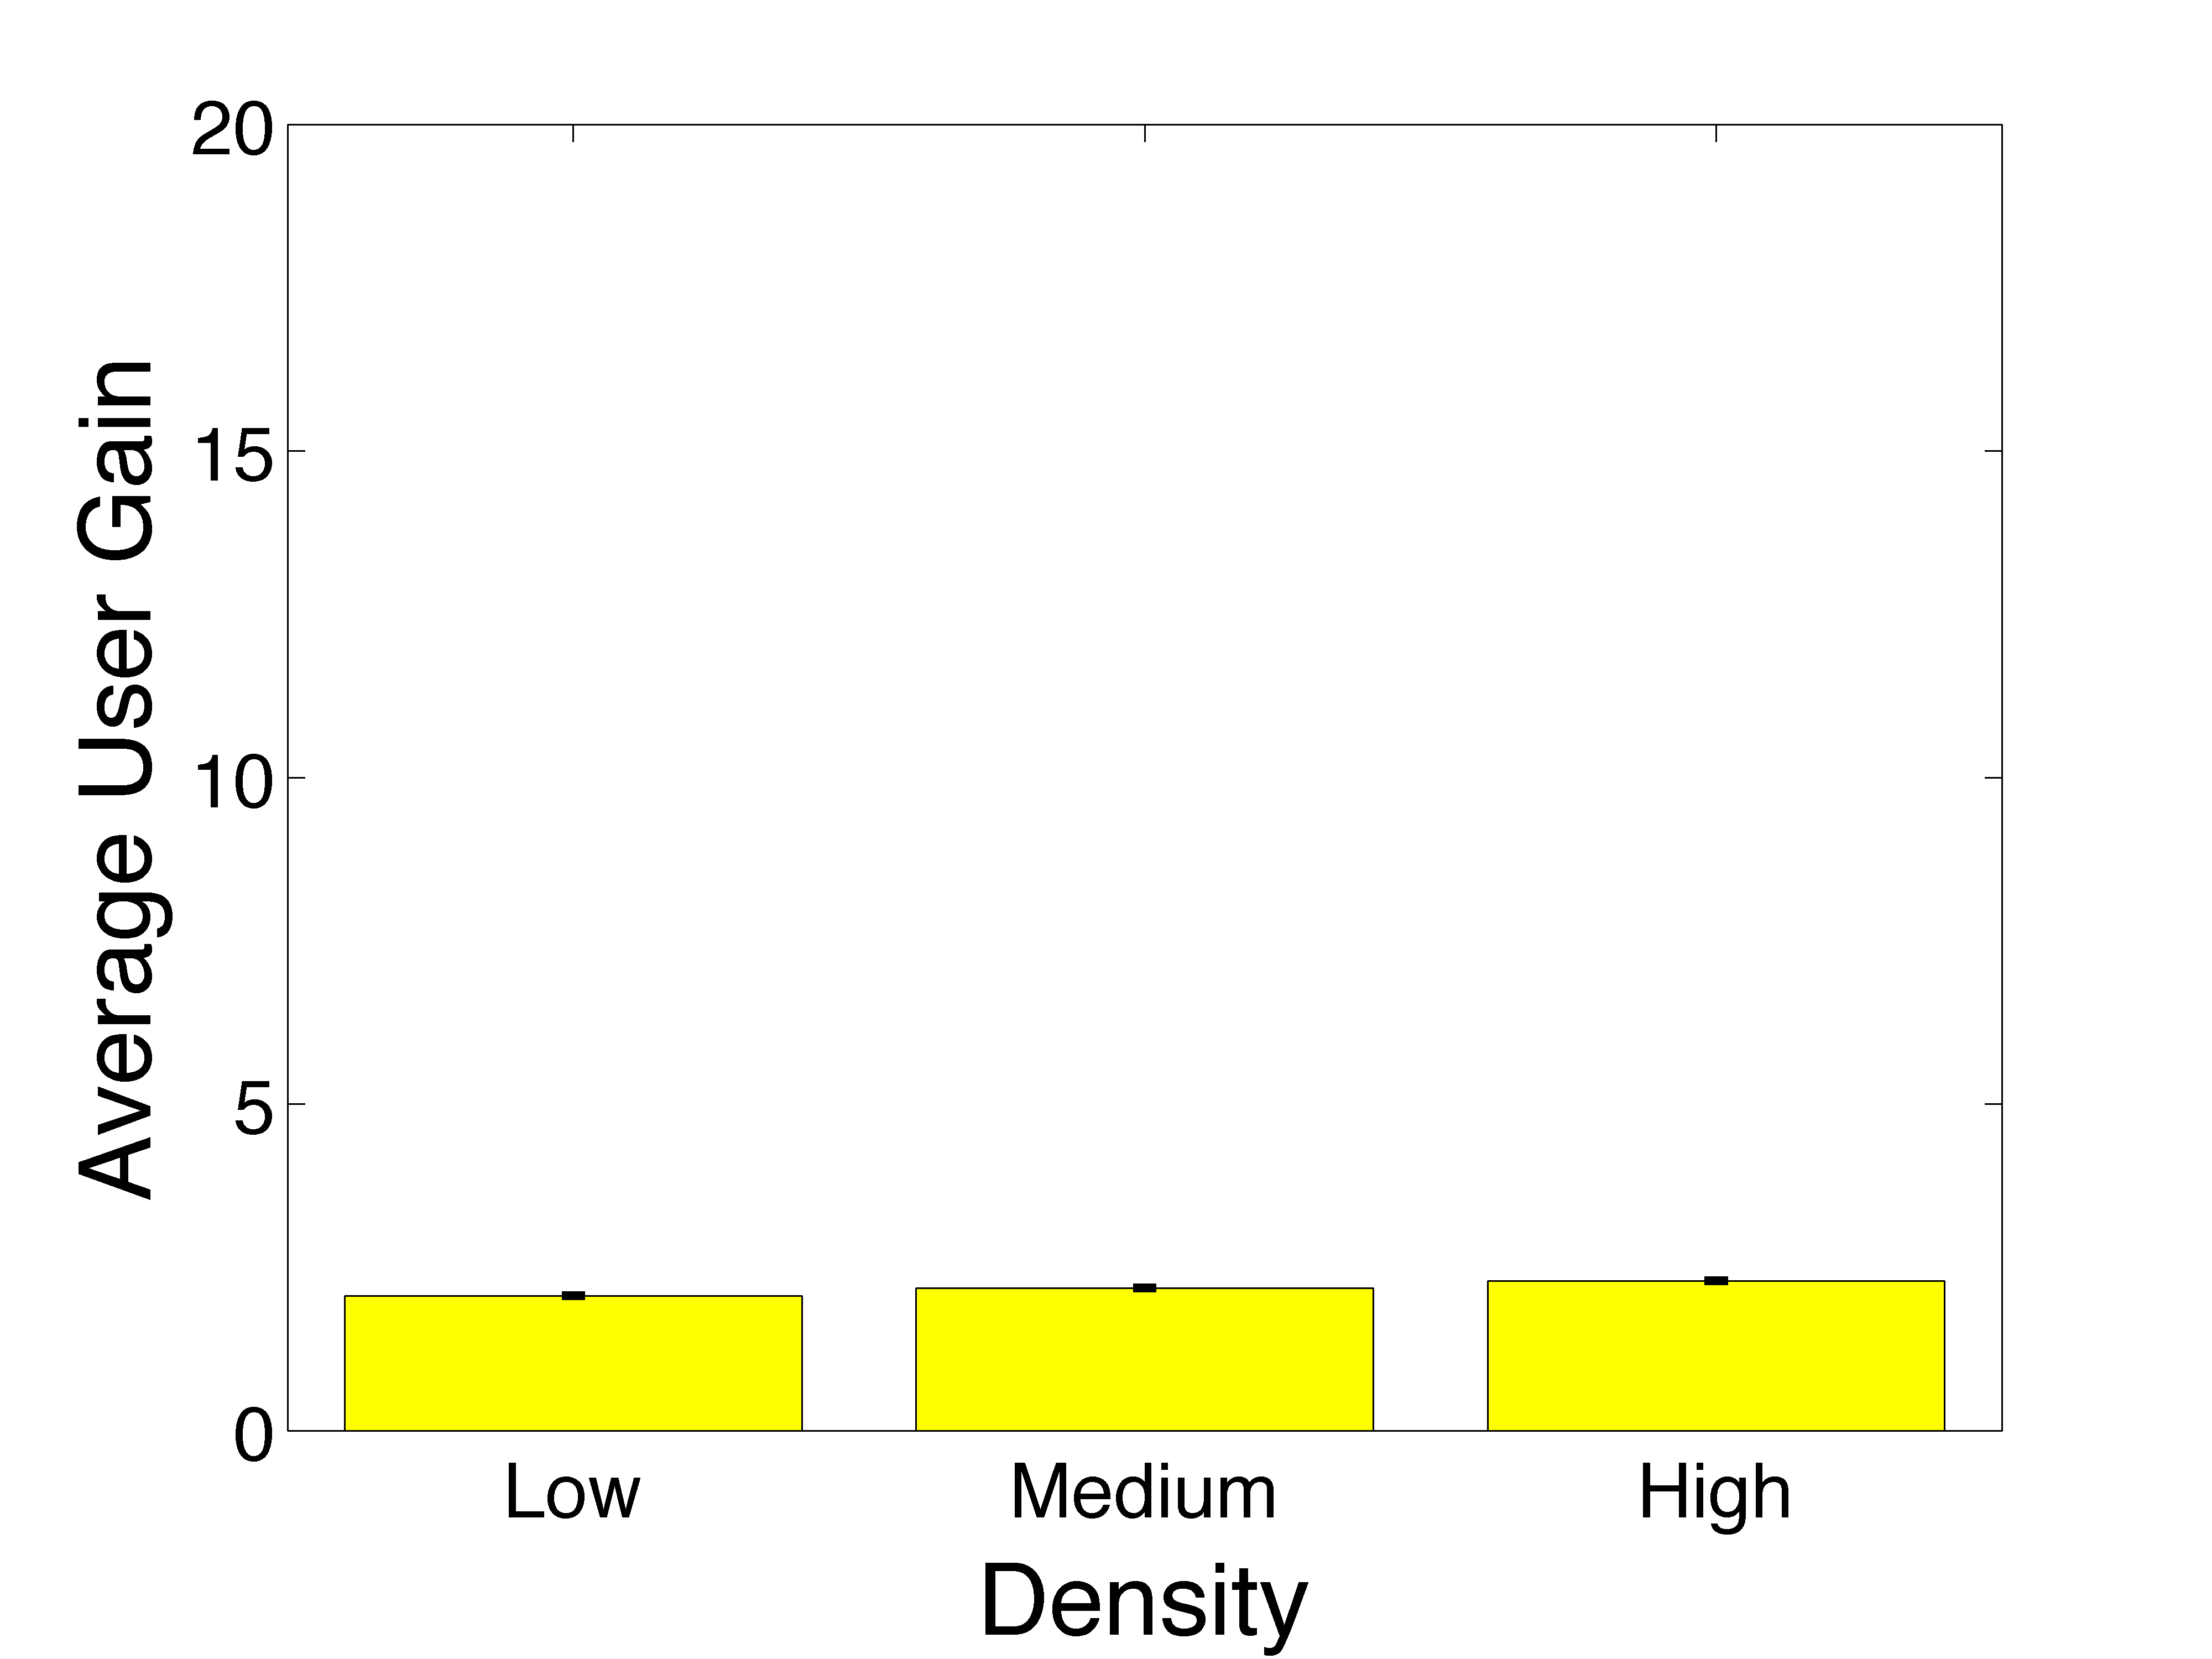
\includegraphics[width=0.33\textwidth,type=png,ext=.png,read=.png]{img/Random-0.500-AUG}
% 	}  
%   \hspace{-0.1in}\subfigure[Scale Free.]{
% 	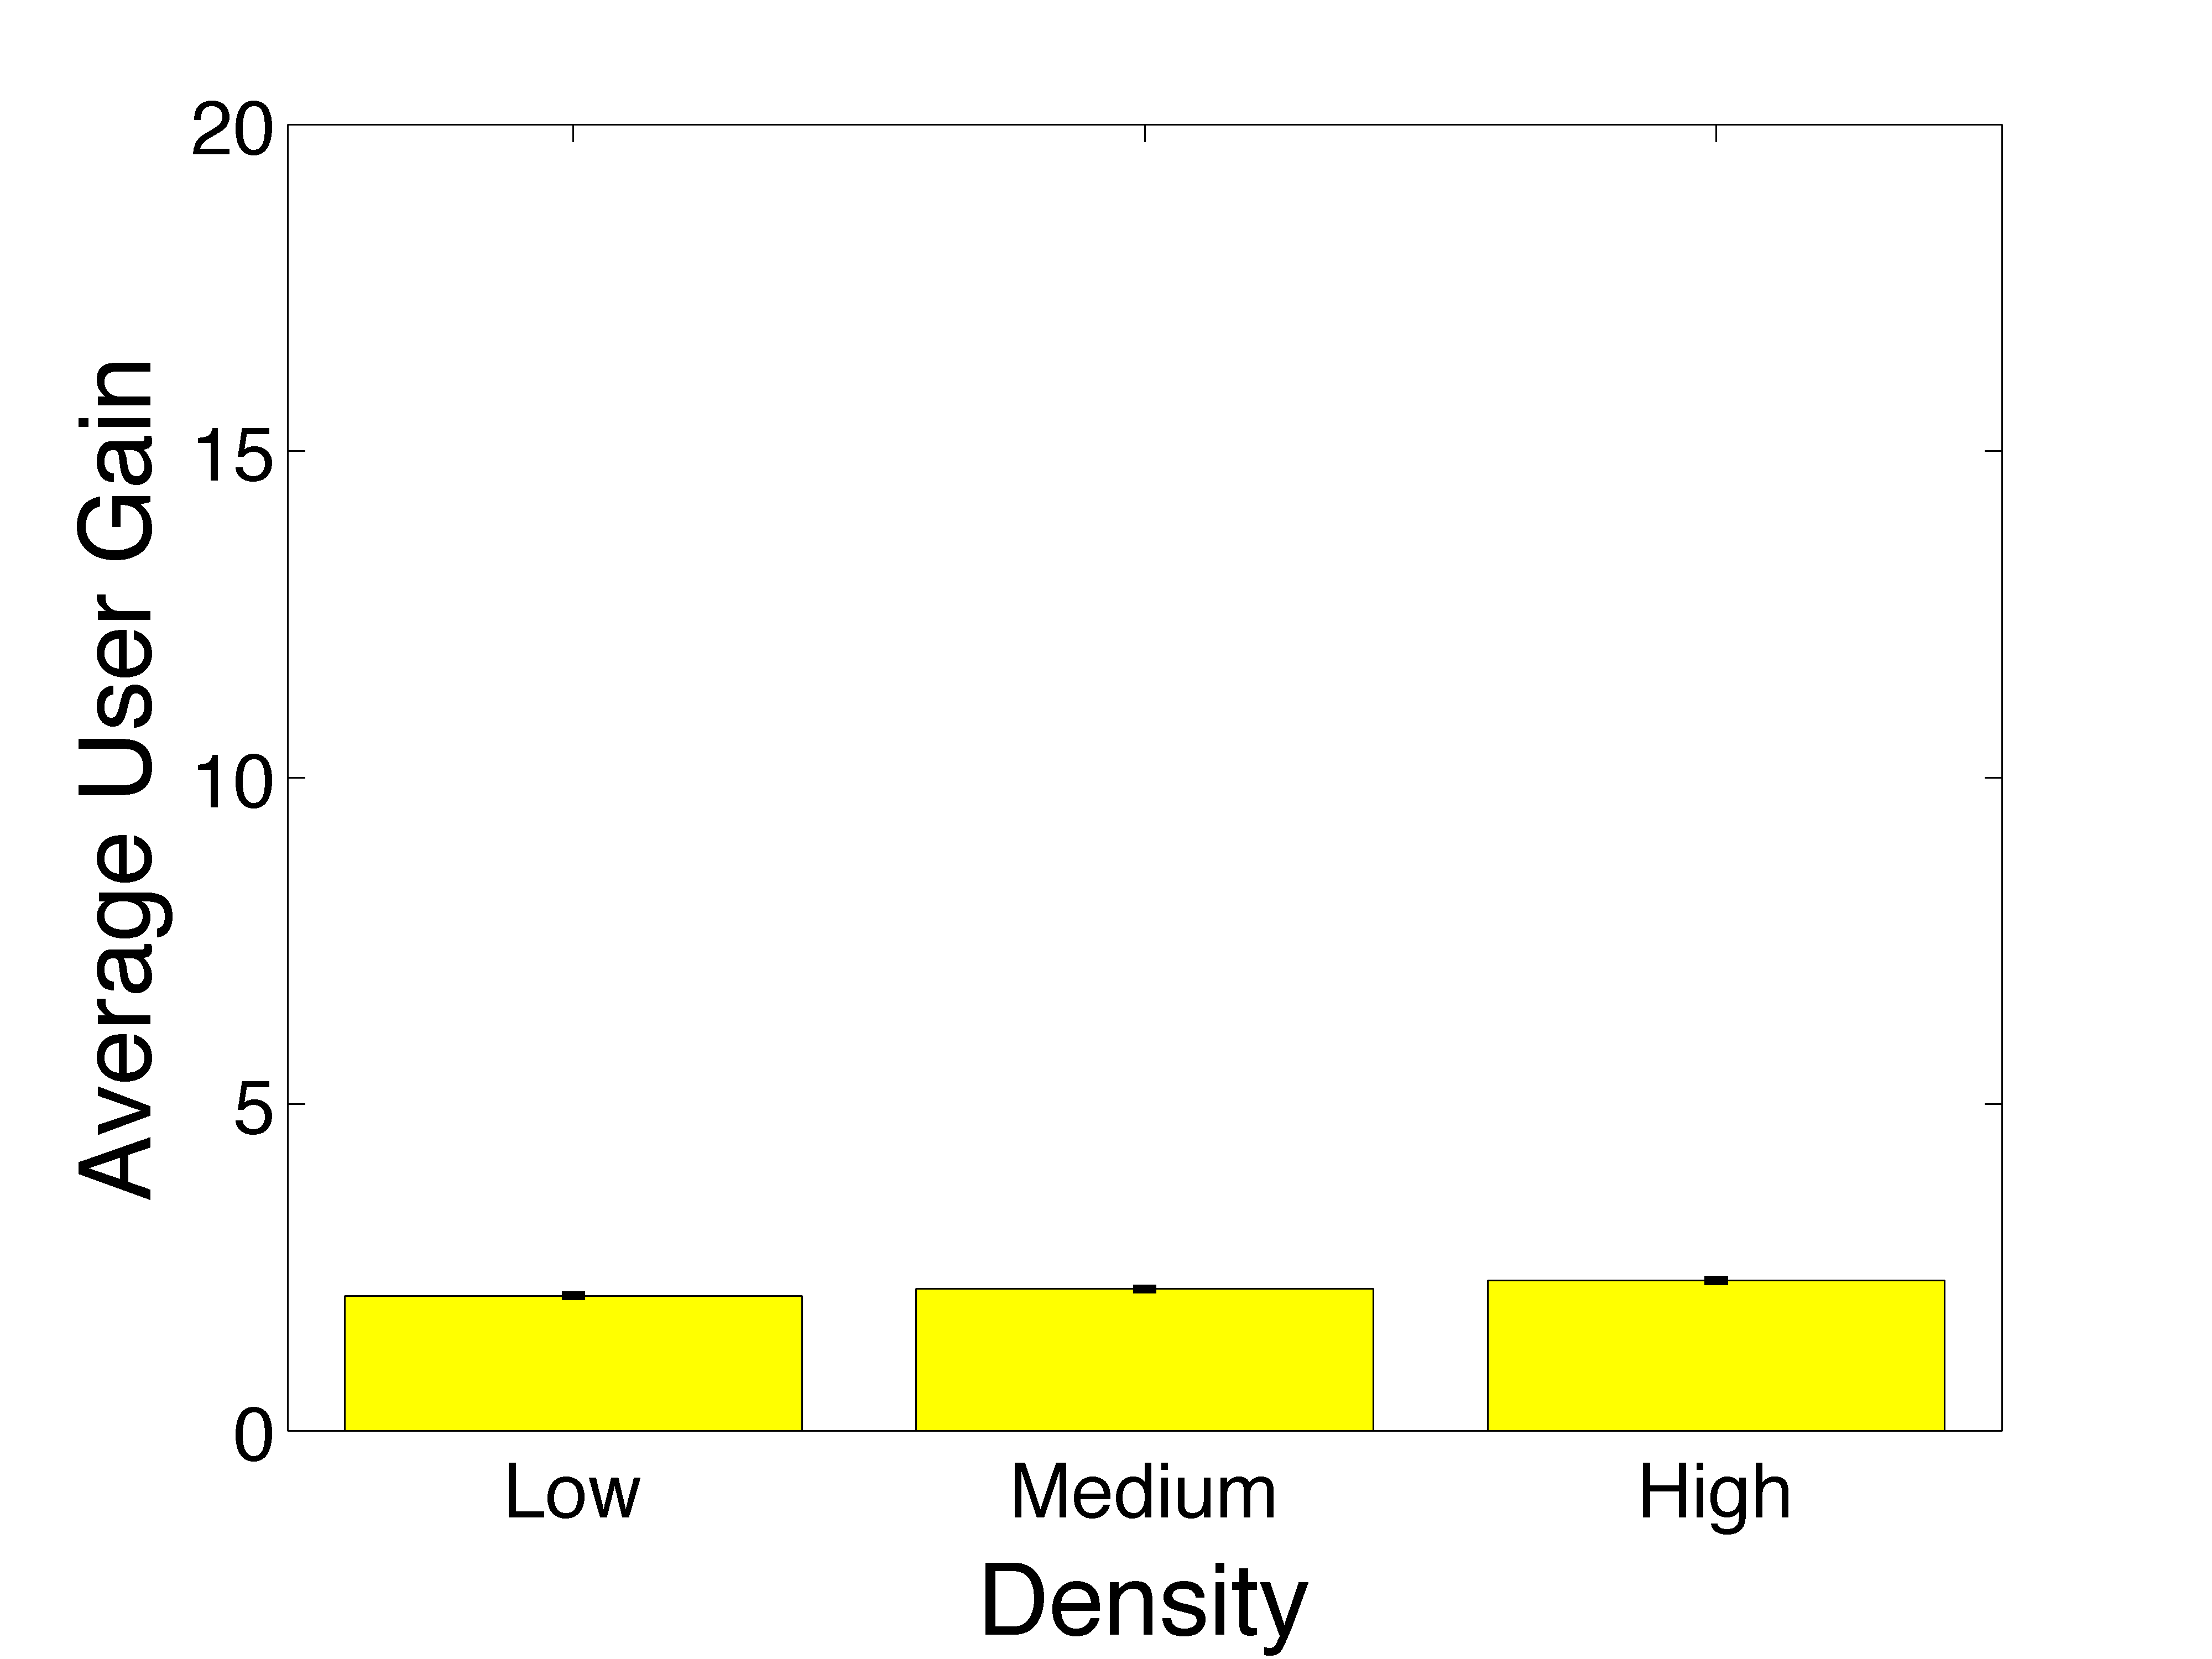
\includegraphics[width=0.33\textwidth,type=png,ext=.png,read=.png]{img/ScaleFree-0.500-AUG}
% 	}  
%   \hspace{-0.1in}\subfigure[Small World.]{
%   	%\label{fig:res_mmuca_time}
% 	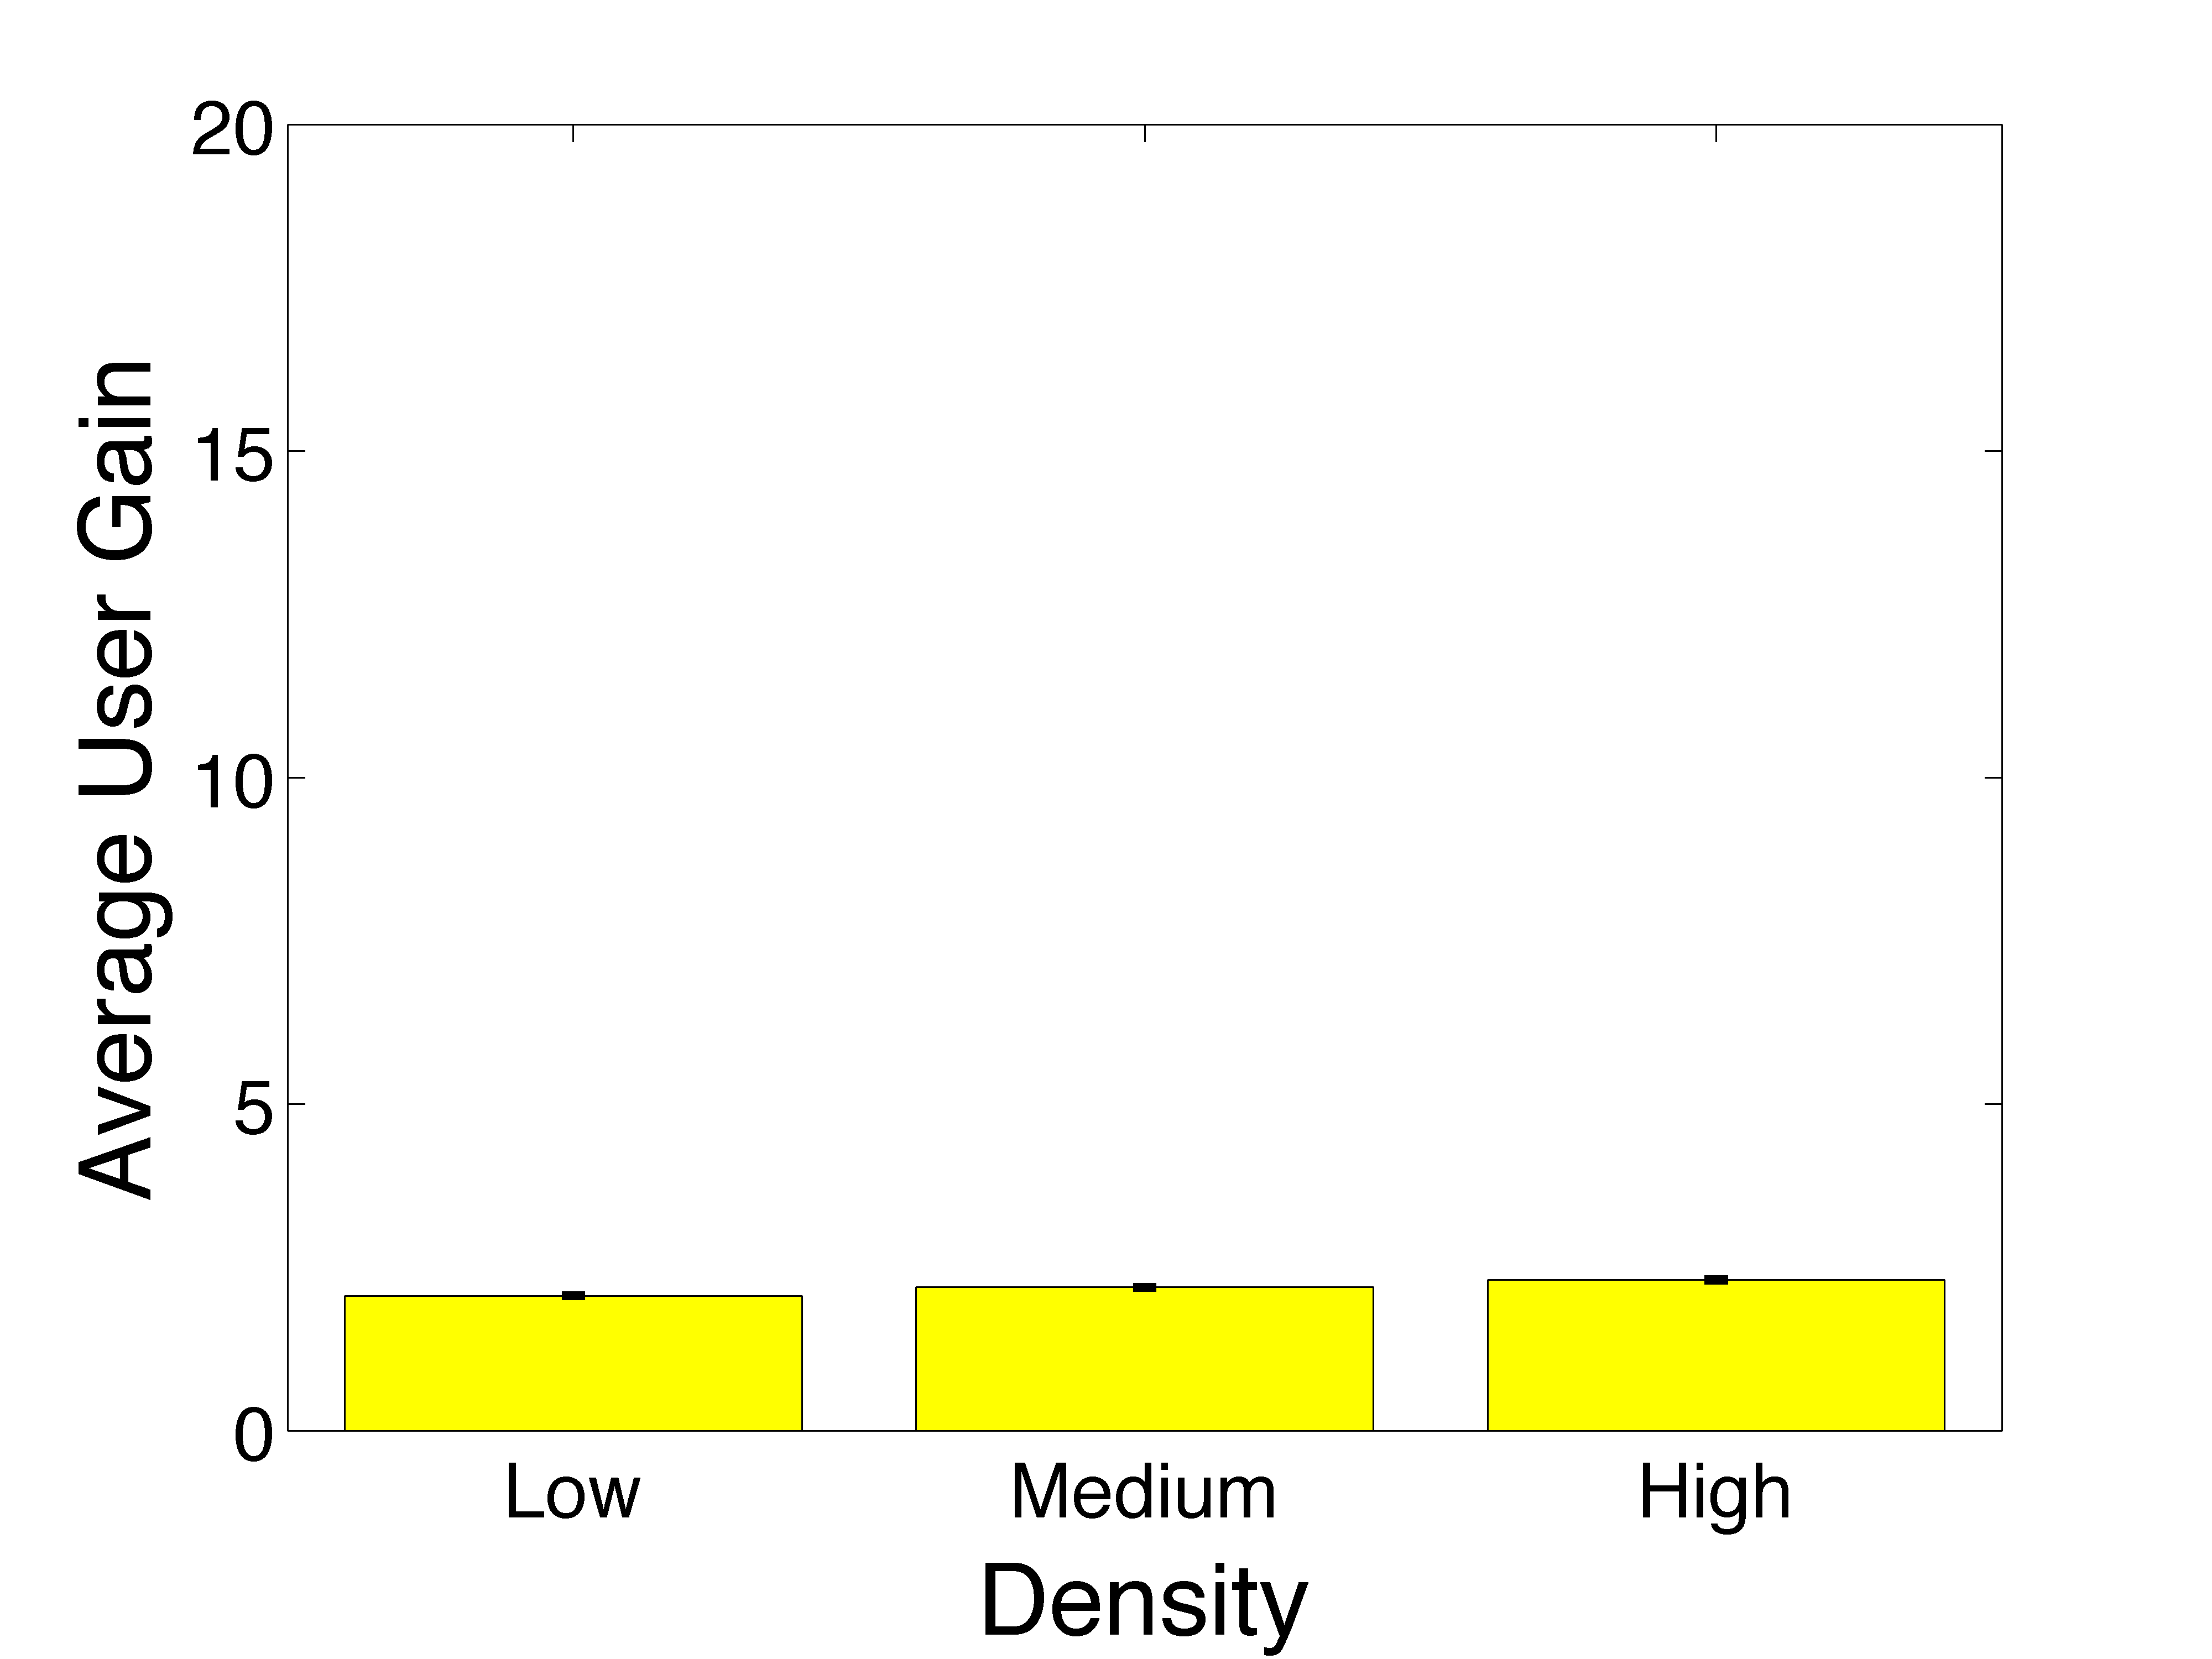
\includegraphics[width=0.33\textwidth,type=png,ext=.png,read=.png]{img/SmallWorld-0.500-AUG}
% 	}    
%   \caption{$ p=0.500$ Graphs showing the average percent gain of consumers'
%   payoffs in the coalitions with respect to the payoff of individual coalitions on
%   different topologies and with different densities. }
%   \label{fig:graphs_gain}
% \end{figure*}

% \begin{figure*}
%   \centering  
%   \hspace{-0.1in}\subfigure[Random Graphs.]{
%   	%\label{fig:res_walsh_bandwidth}
% 	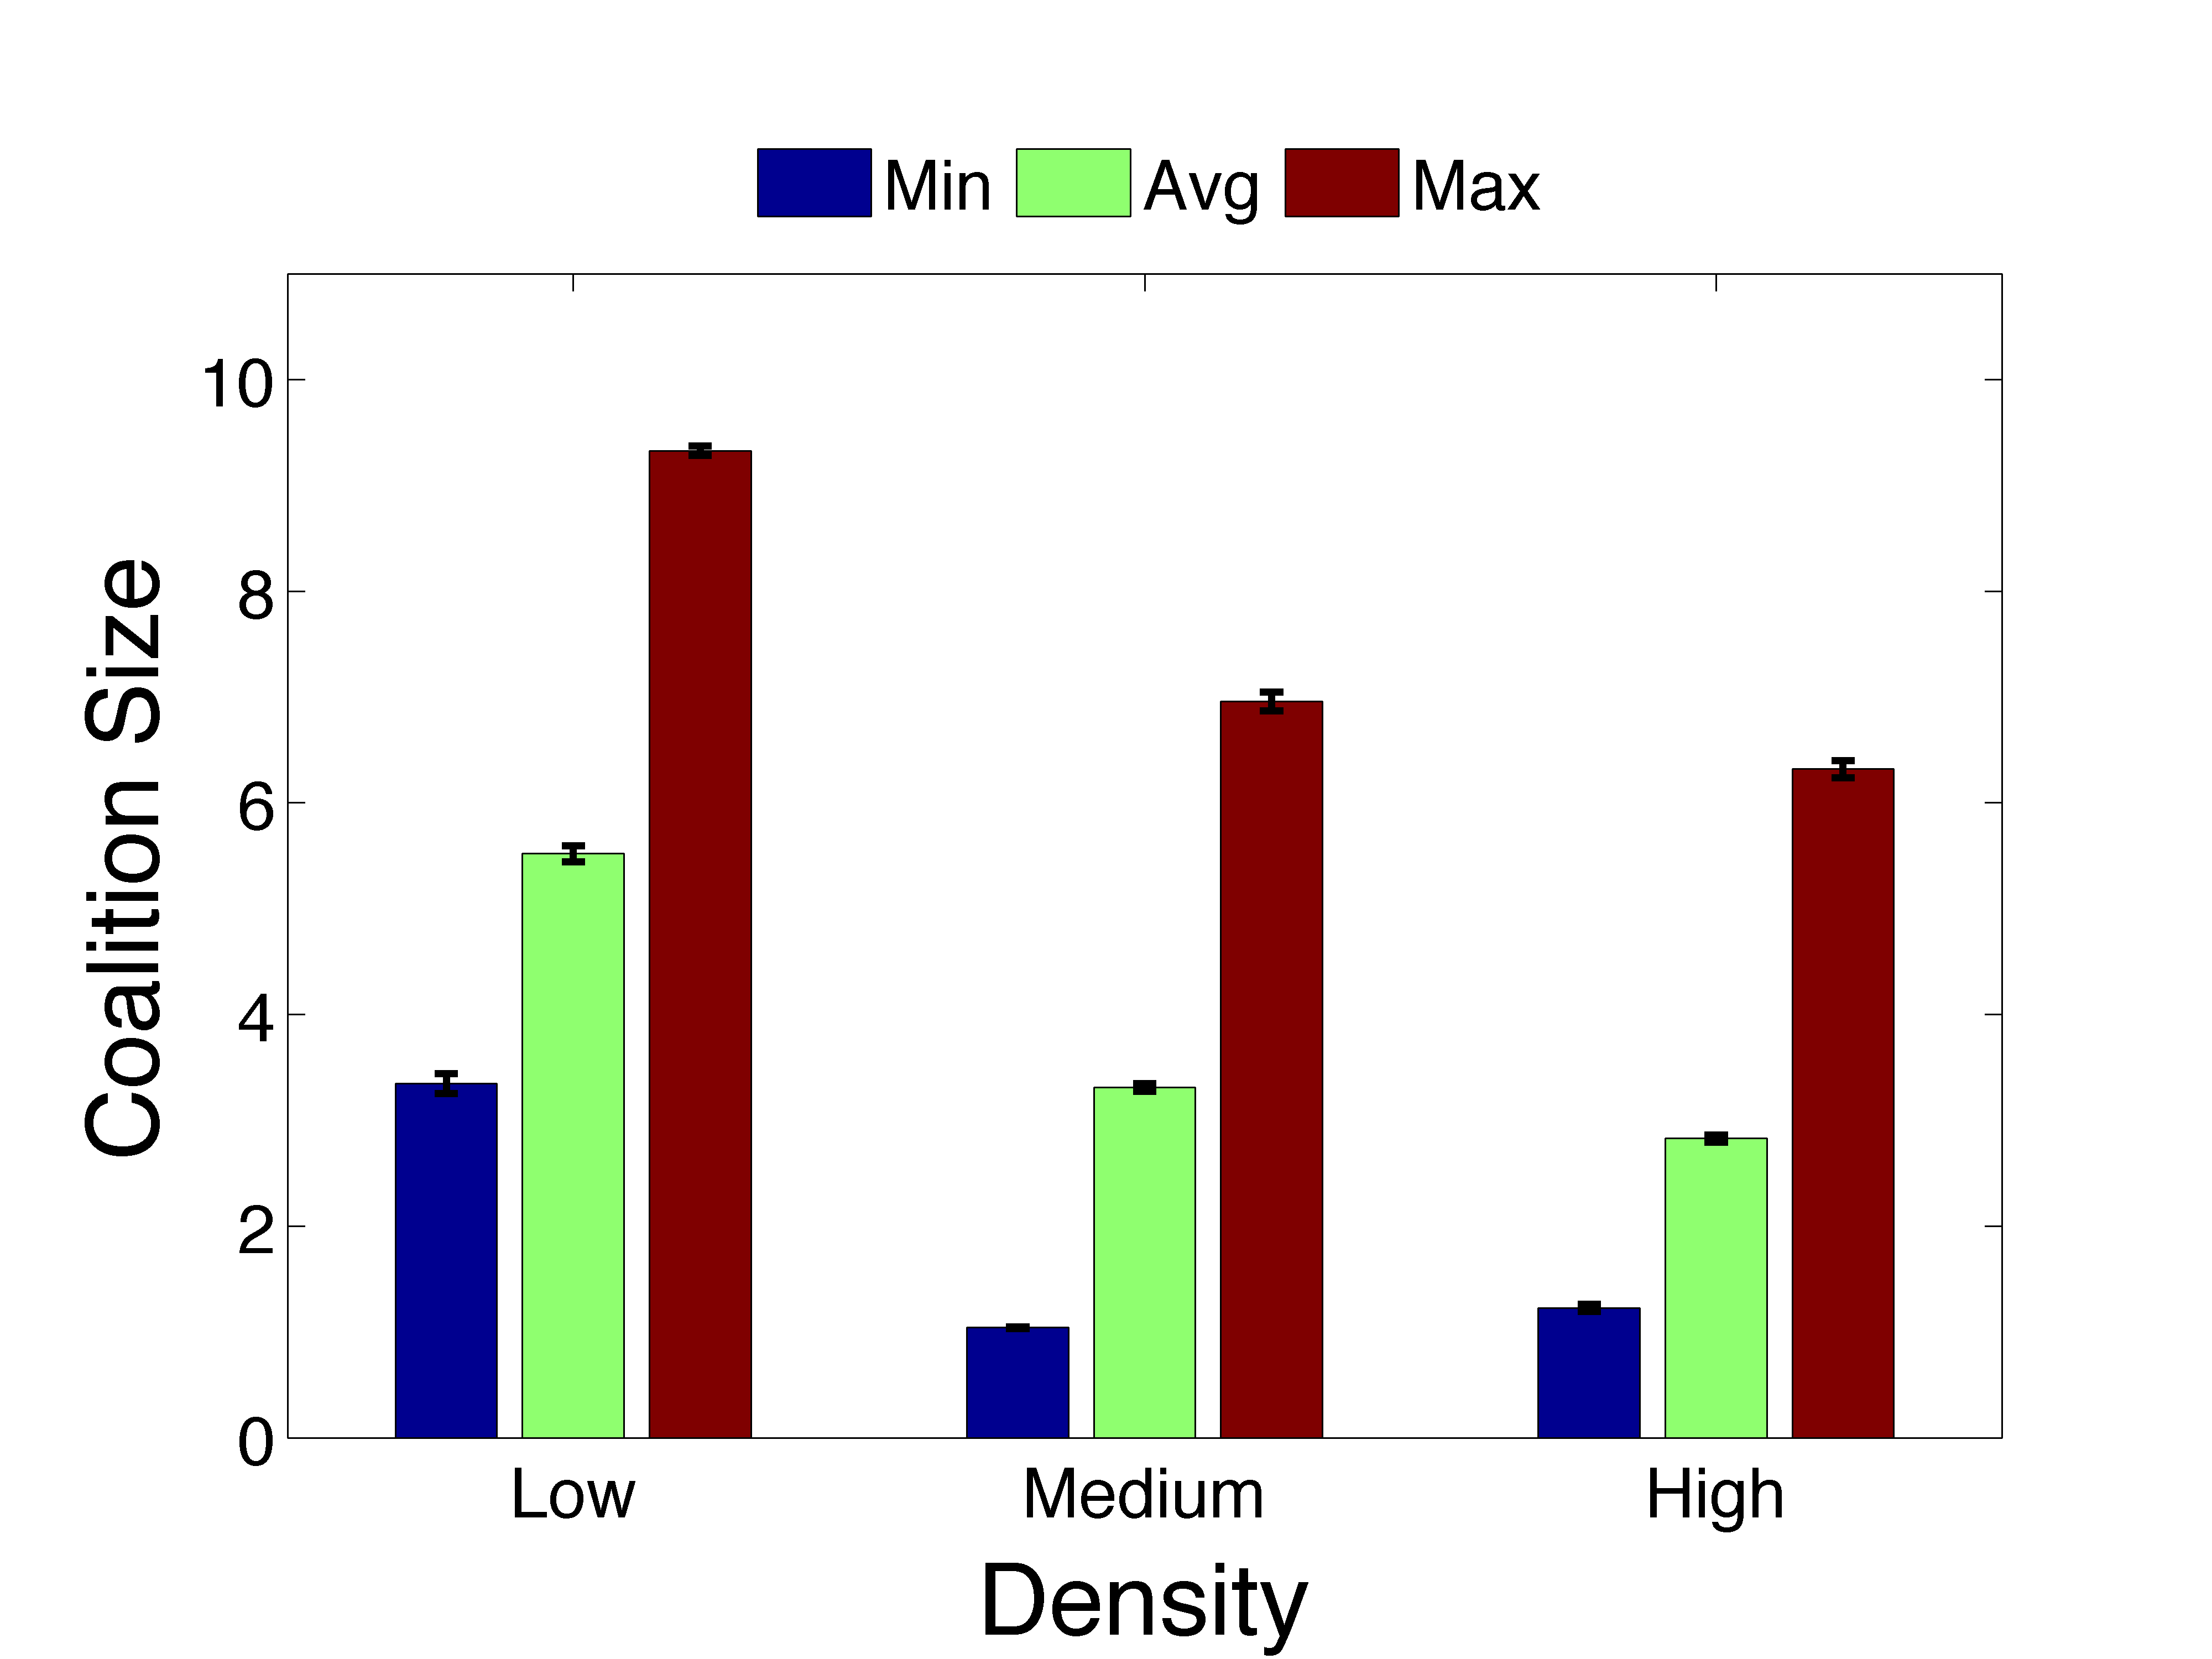
\includegraphics[width=0.33\textwidth,type=png,ext=.png,read=.png]{img/Random-1.000-Size}
% 	}
%   \hspace{-0.1in}\subfigure[Scale Free.]{
%   	%\label{fig:res_mmuca_bandwidth}
% 	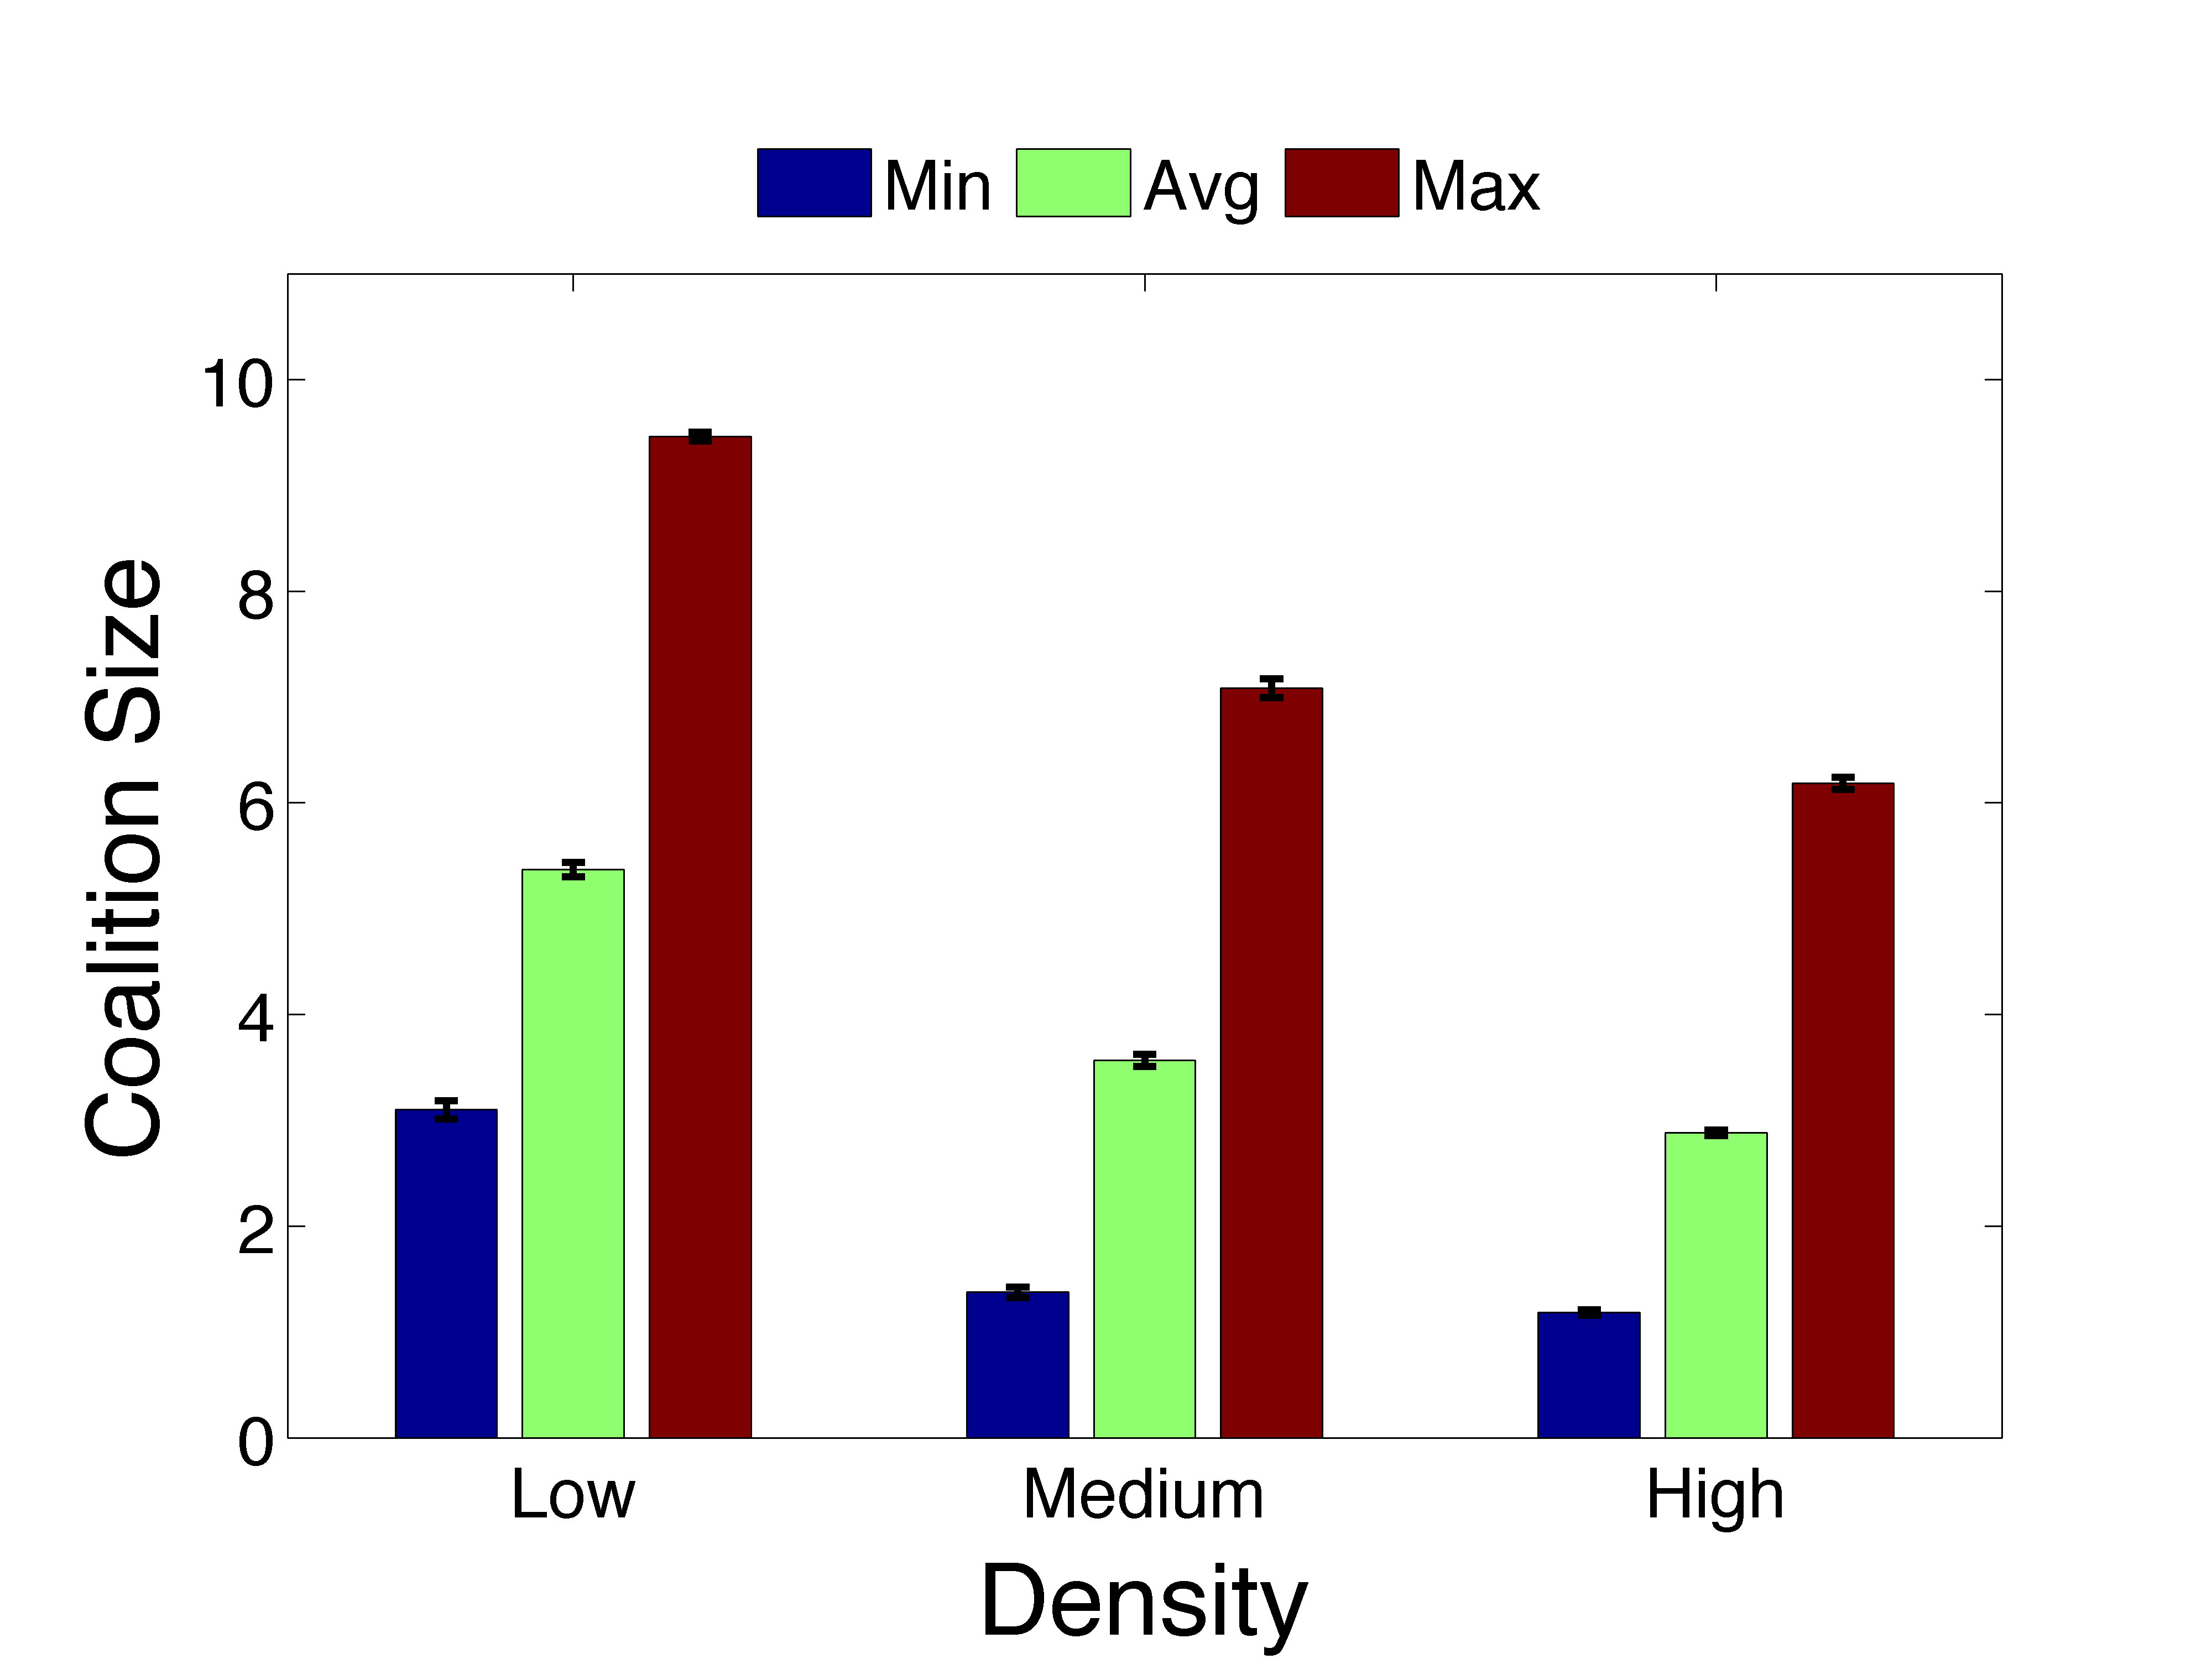
\includegraphics[width=0.33\textwidth,type=png,ext=.png,read=.png]{img/ScaleFree-1.000-Size}
% 	}
%   \hspace{-0.1in}\subfigure[Small World.]{
%   	%\label{fig:res_mmuca_quality}
% 	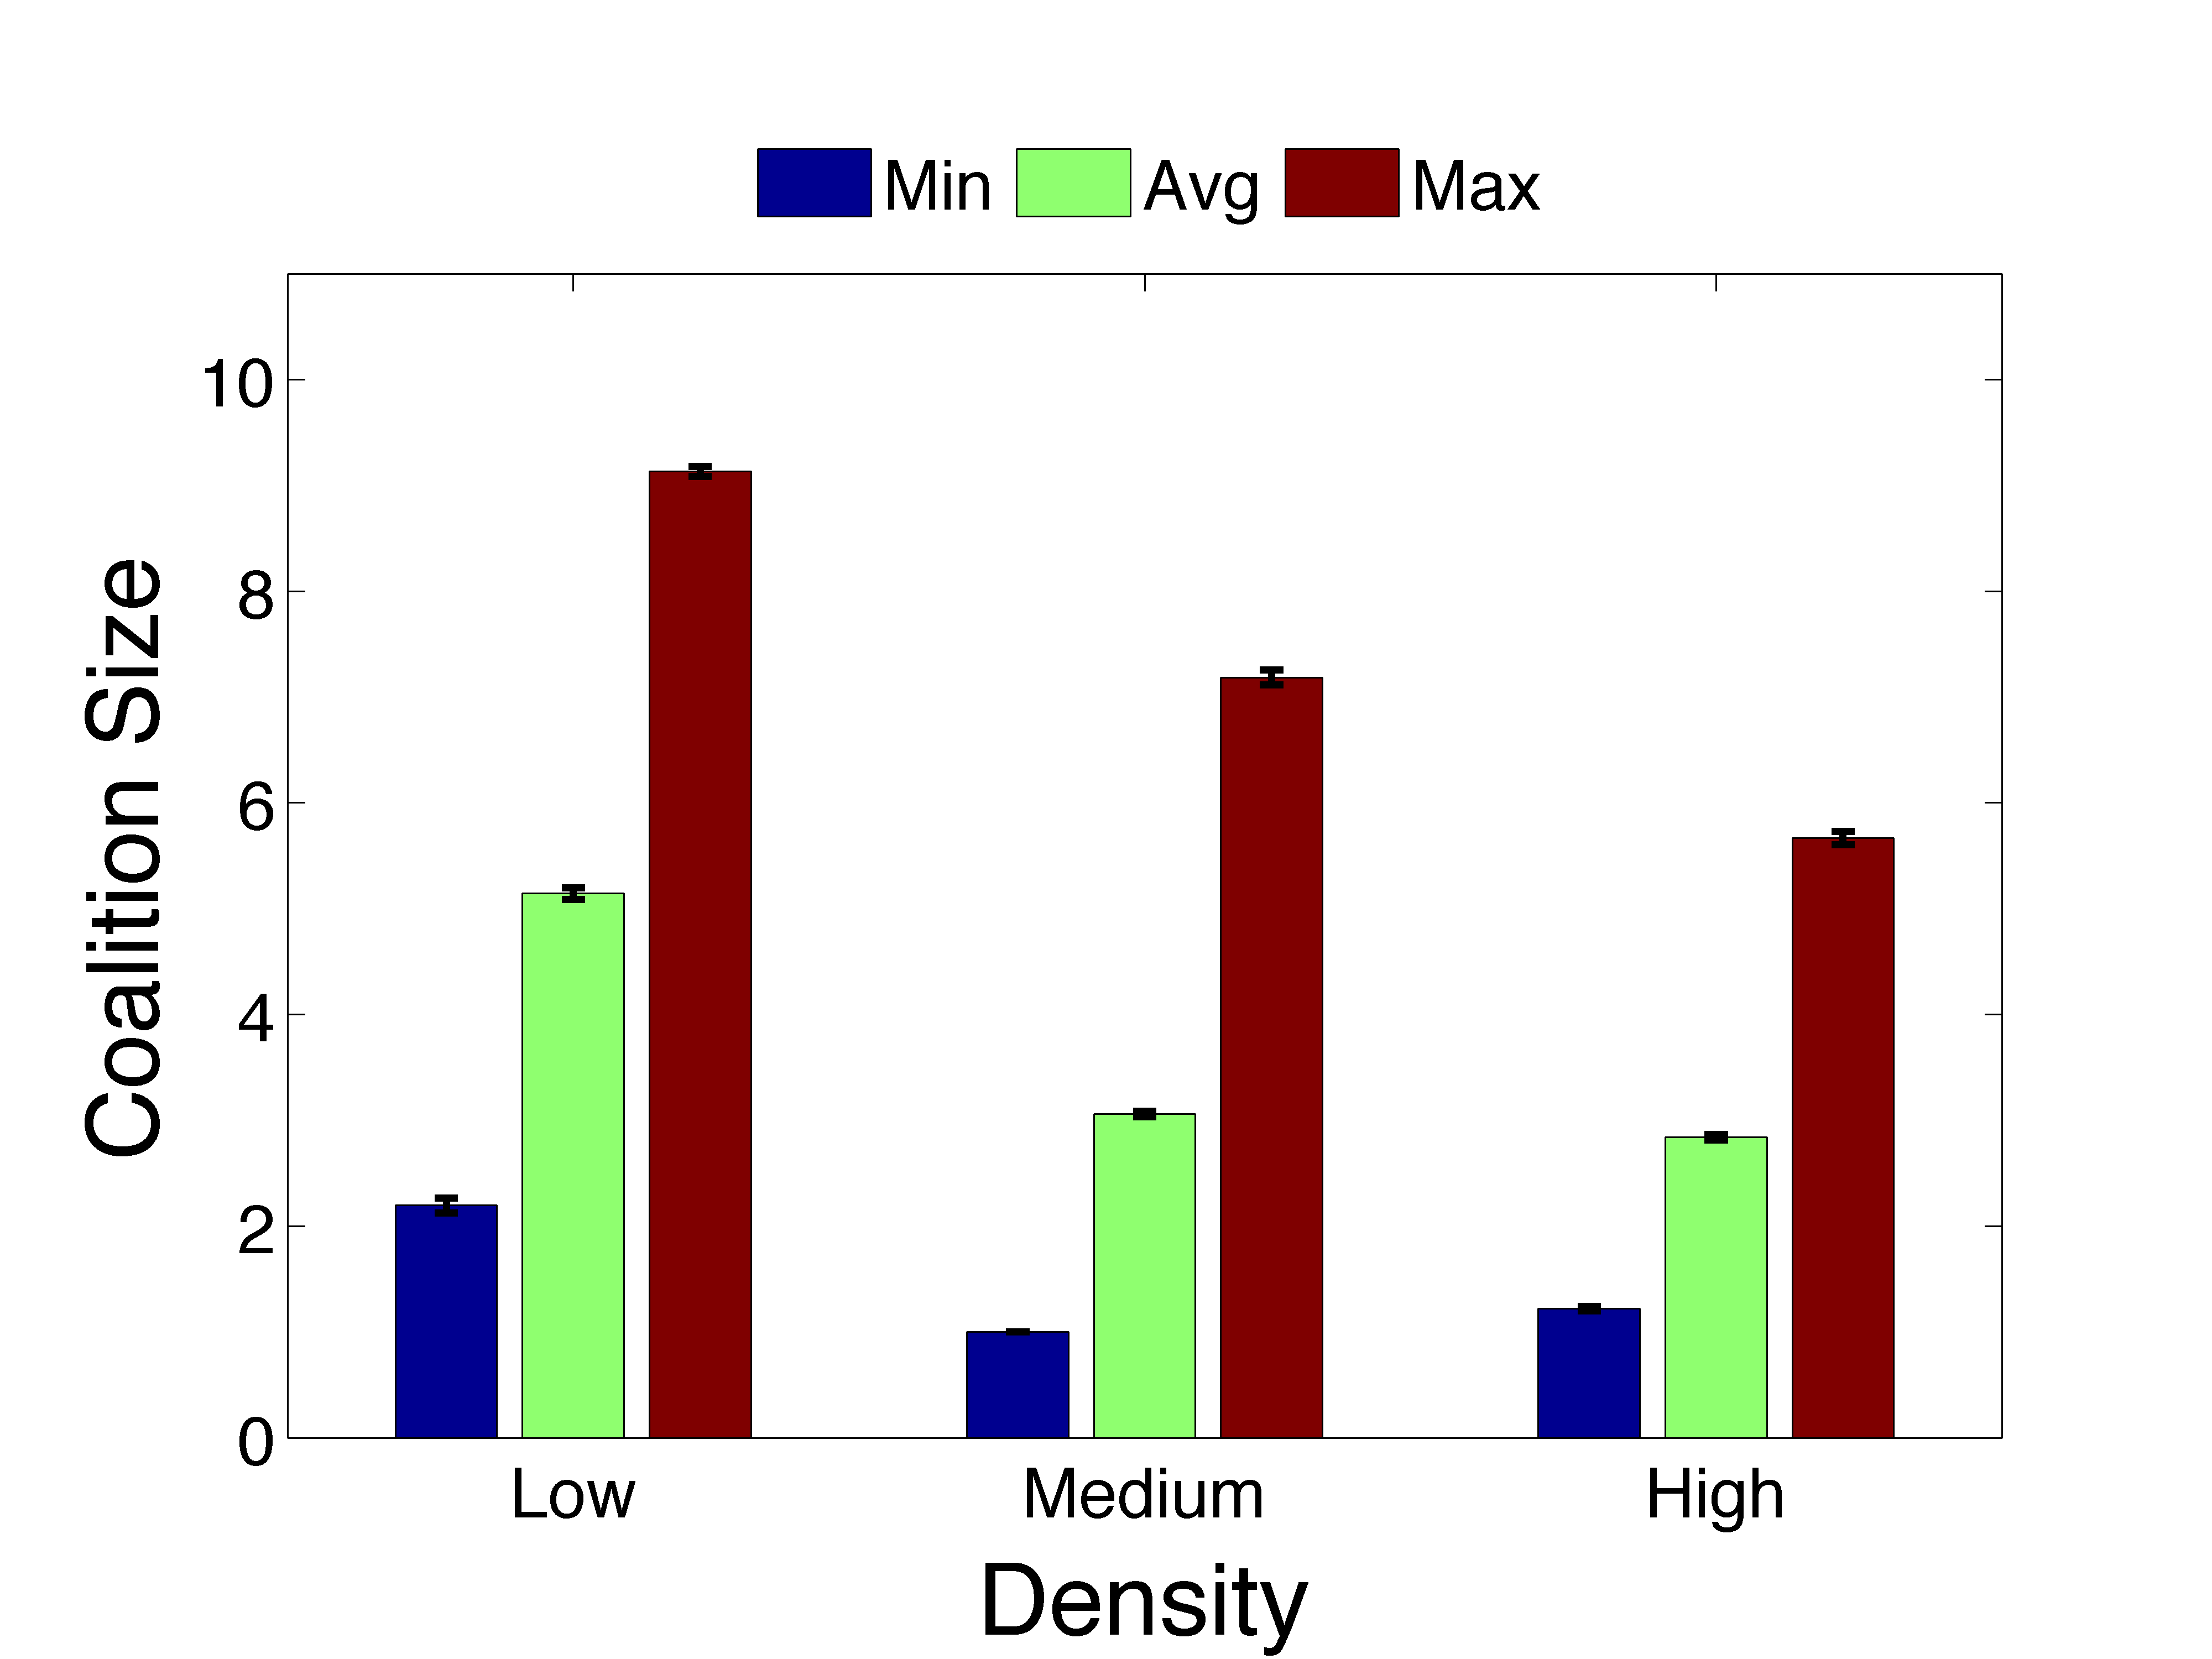
\includegraphics[width=0.33\textwidth,type=png,ext=.png,read=.png]{img/SmallWorld-1.000-Size}
% 	}  
%   \caption{70/80 p=1 Graphs showing the minimum, average and maximum size of
%   coalitions formed on different topologies and with different densities. }
%   \label{fig:graphs_size}
% \end{figure*}
\subsubsection{Structure of energy coalitions}
In this section we analyse the structure of the energy coalitions obtained in
the experiments. For each configuration, we plot the mean of the minimum,
average and maximum size of coalitions formed. Figure \ref{fig:graphs_size}
plots the results for networks of 12 agents on a random, scale free and
small-world networks in two different market scenarios. We also plotted
the standard error of the mean as a measure of the variance in each graph.
Market scenario M3 is omitted because in this case we detected that the gran coalition was always formed in all tested instances.
In contrast we observe that for markets M1 and M2, the market conditions lead to
coalitions of middle size in all network structures. We also observe that as we
increase the density of the network, more coalitions of middle size are composed
whereas in low densities agents tend to compose larger coalitions.


\begin{figure*}
  \centering
  \hspace{-0.1in}\subfigure[Random Graphs M1.]{
  	%\label{fig:res_walsh_bandwidth}
	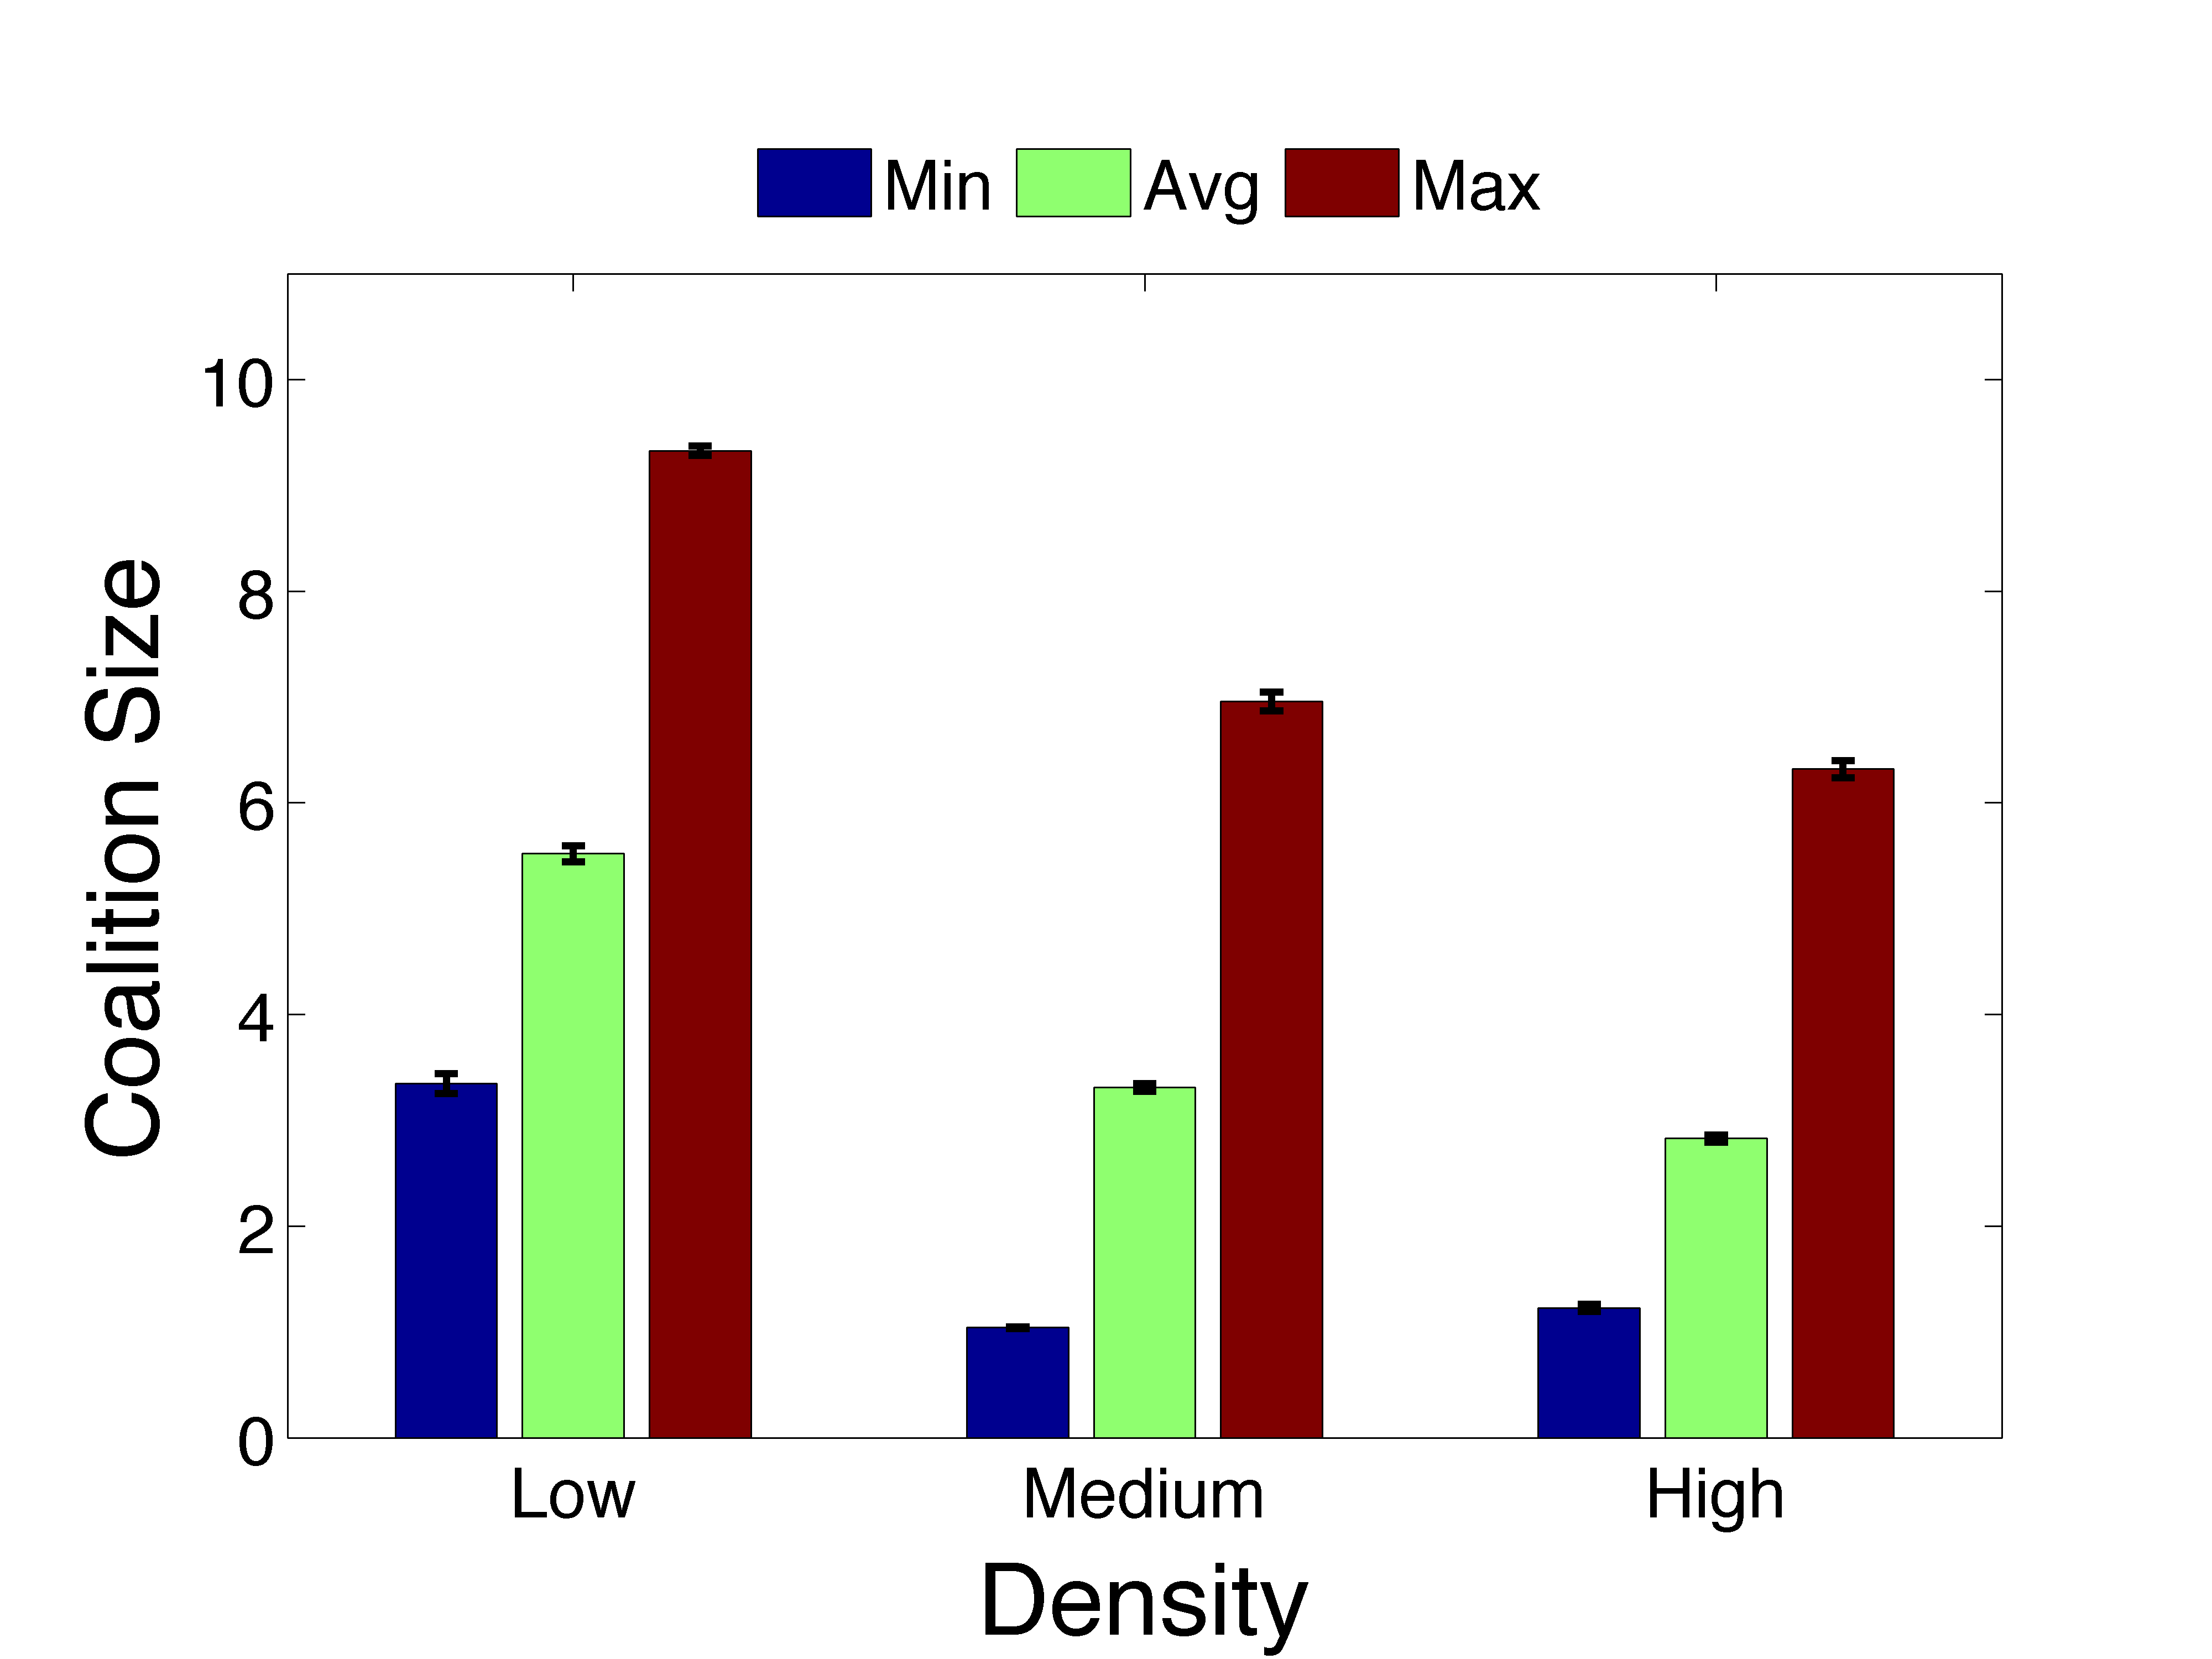
\includegraphics[width=0.3\textwidth,type=png,ext=.png,read=.png]{img/Random-1.000-Size}
	}
  \hspace{-0.1in}\subfigure[Scale Free M1.]{
  	%\label{fig:res_mmuca_bandwidth}
	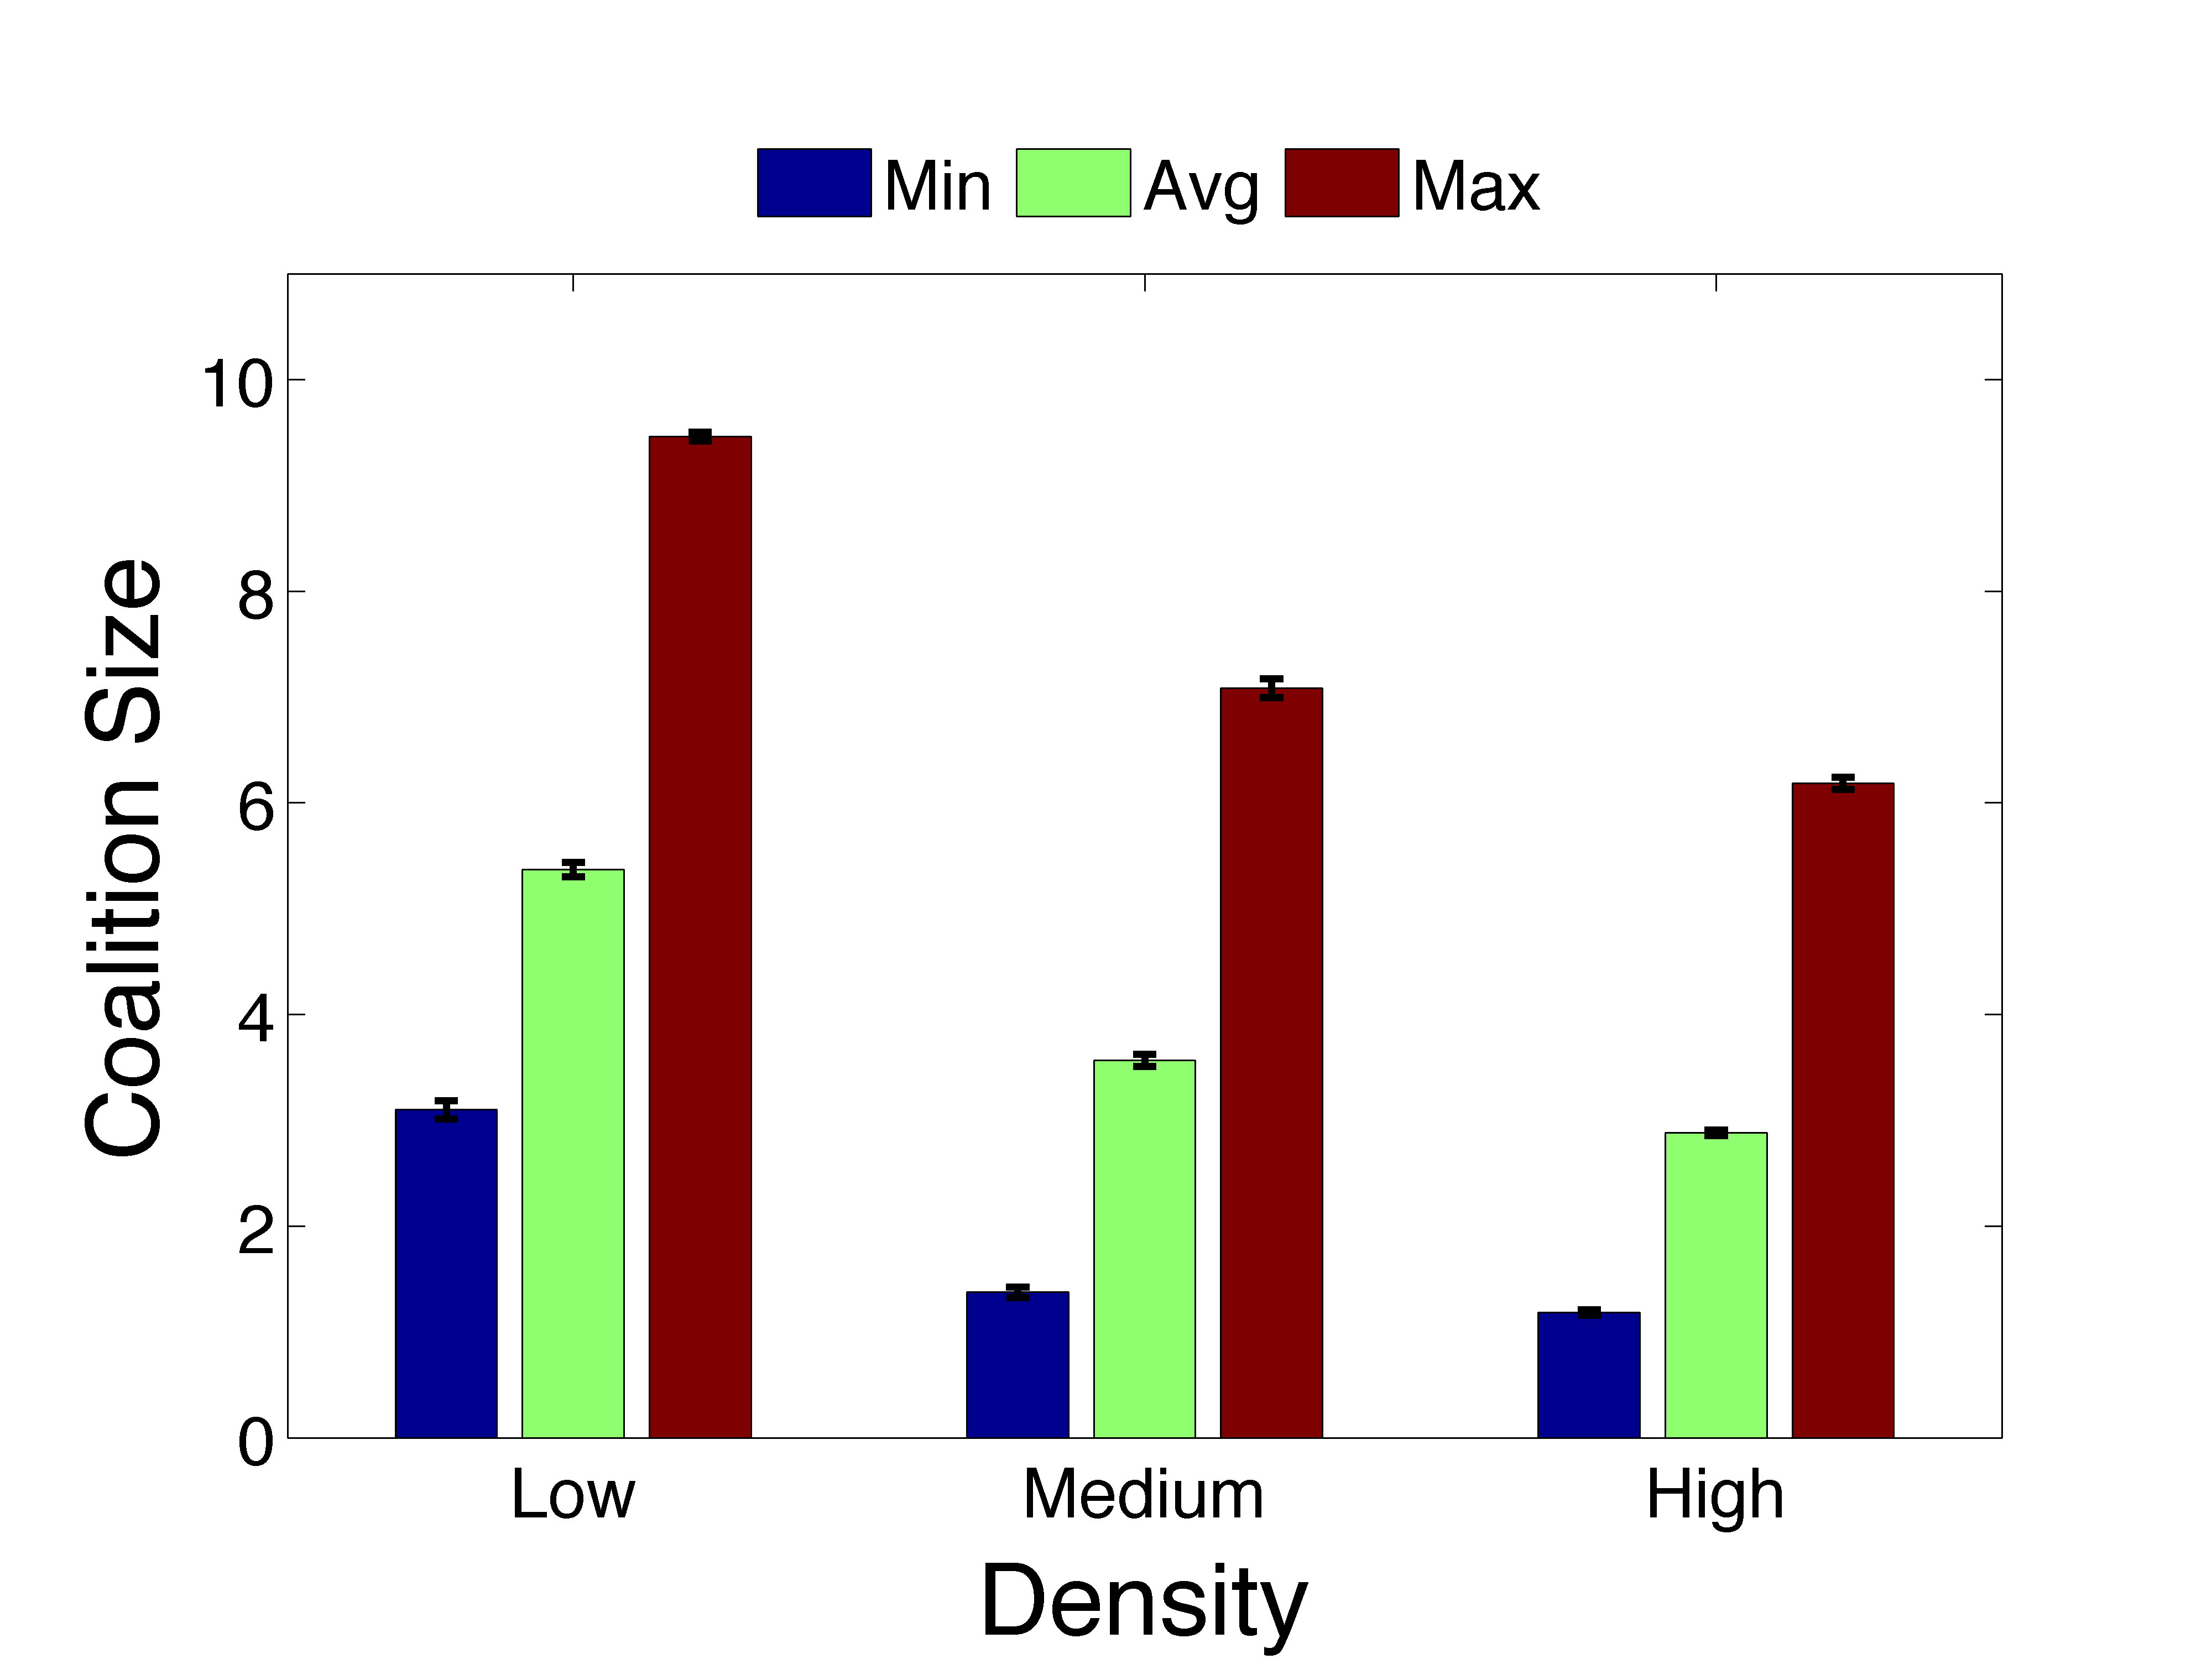
\includegraphics[width=0.3\textwidth,type=png,ext=.png,read=.png]{img/ScaleFree-1.000-Size}
	}  
  \hspace{-0.1in}\subfigure[Small World M1.]{
  	%\label{fig:res_mmuca_quality}
	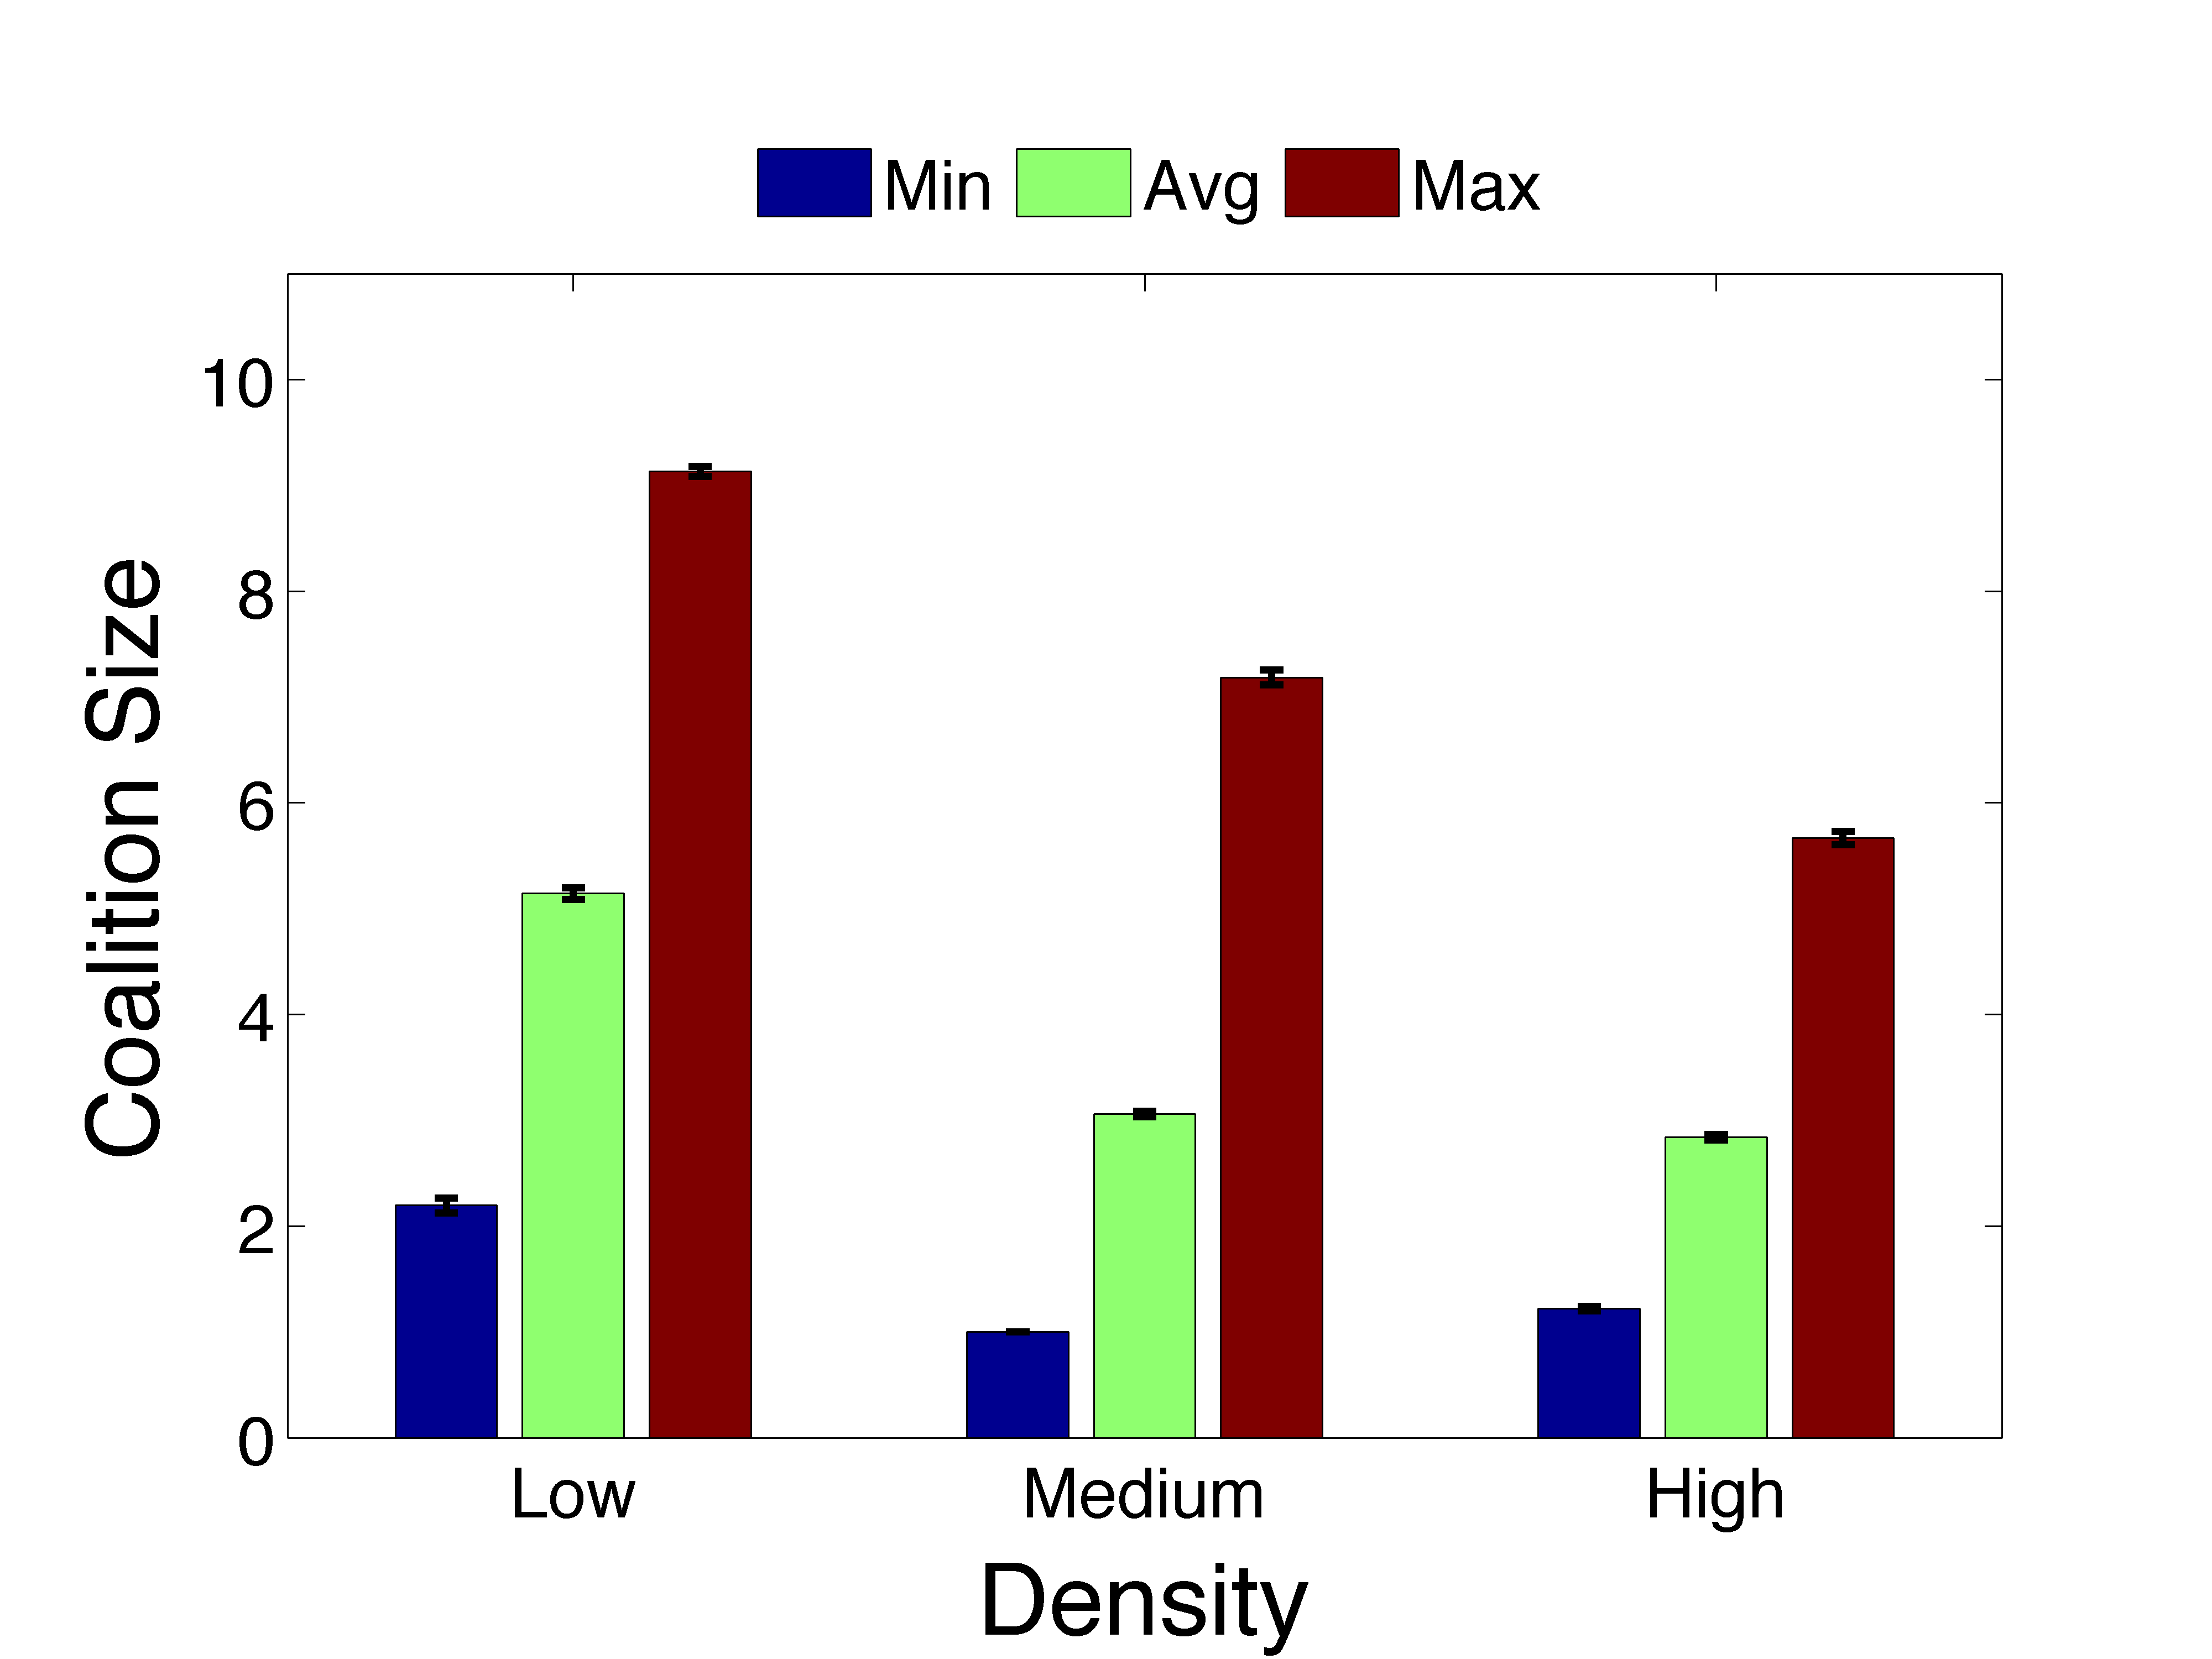
\includegraphics[width=0.3\textwidth,type=png,ext=.png,read=.png]{img/SmallWorld-1.000-Size}
	}      
  \hspace{-0.1in}\subfigure[Random Graphs M2.]{
  	%\label{fig:res_walsh_bandwidth}
	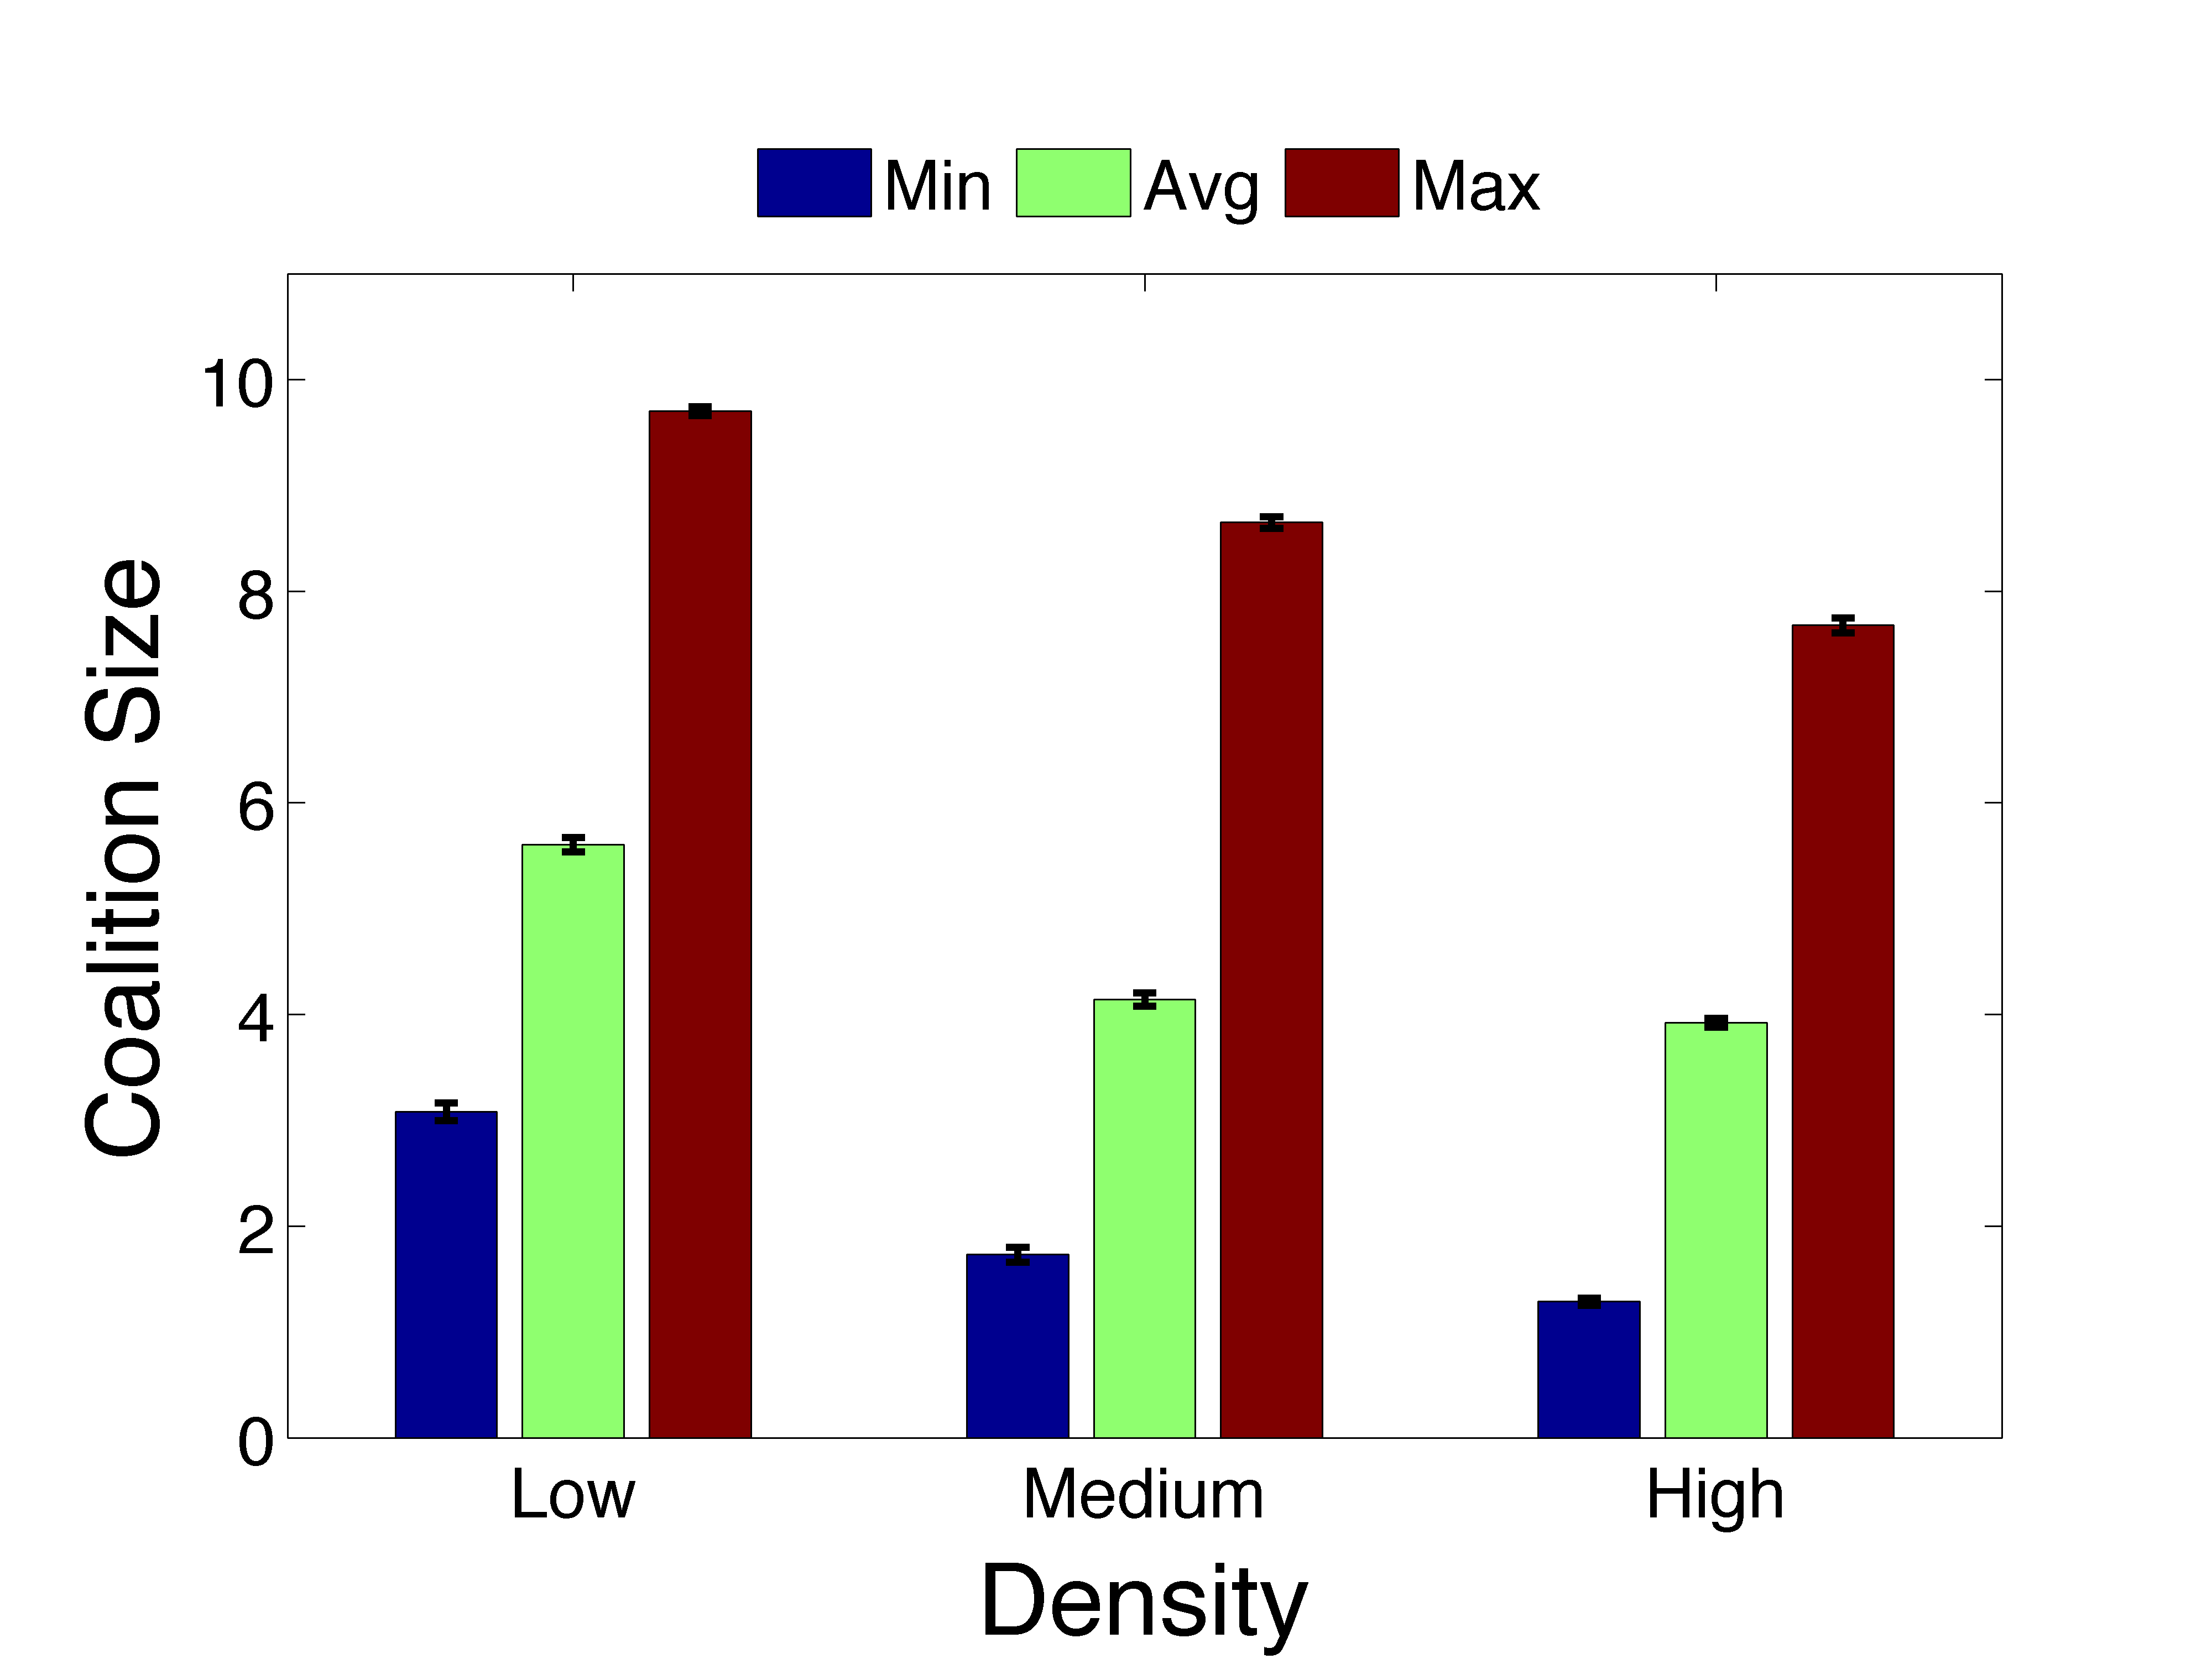
\includegraphics[width=0.3\textwidth,type=png,ext=.png,read=.png]{img/Random-0.875-Size}
	}
  \hspace{-0.1in}\subfigure[Scale Free M2.]{
  	%\label{fig:res_mmuca_bandwidth}
	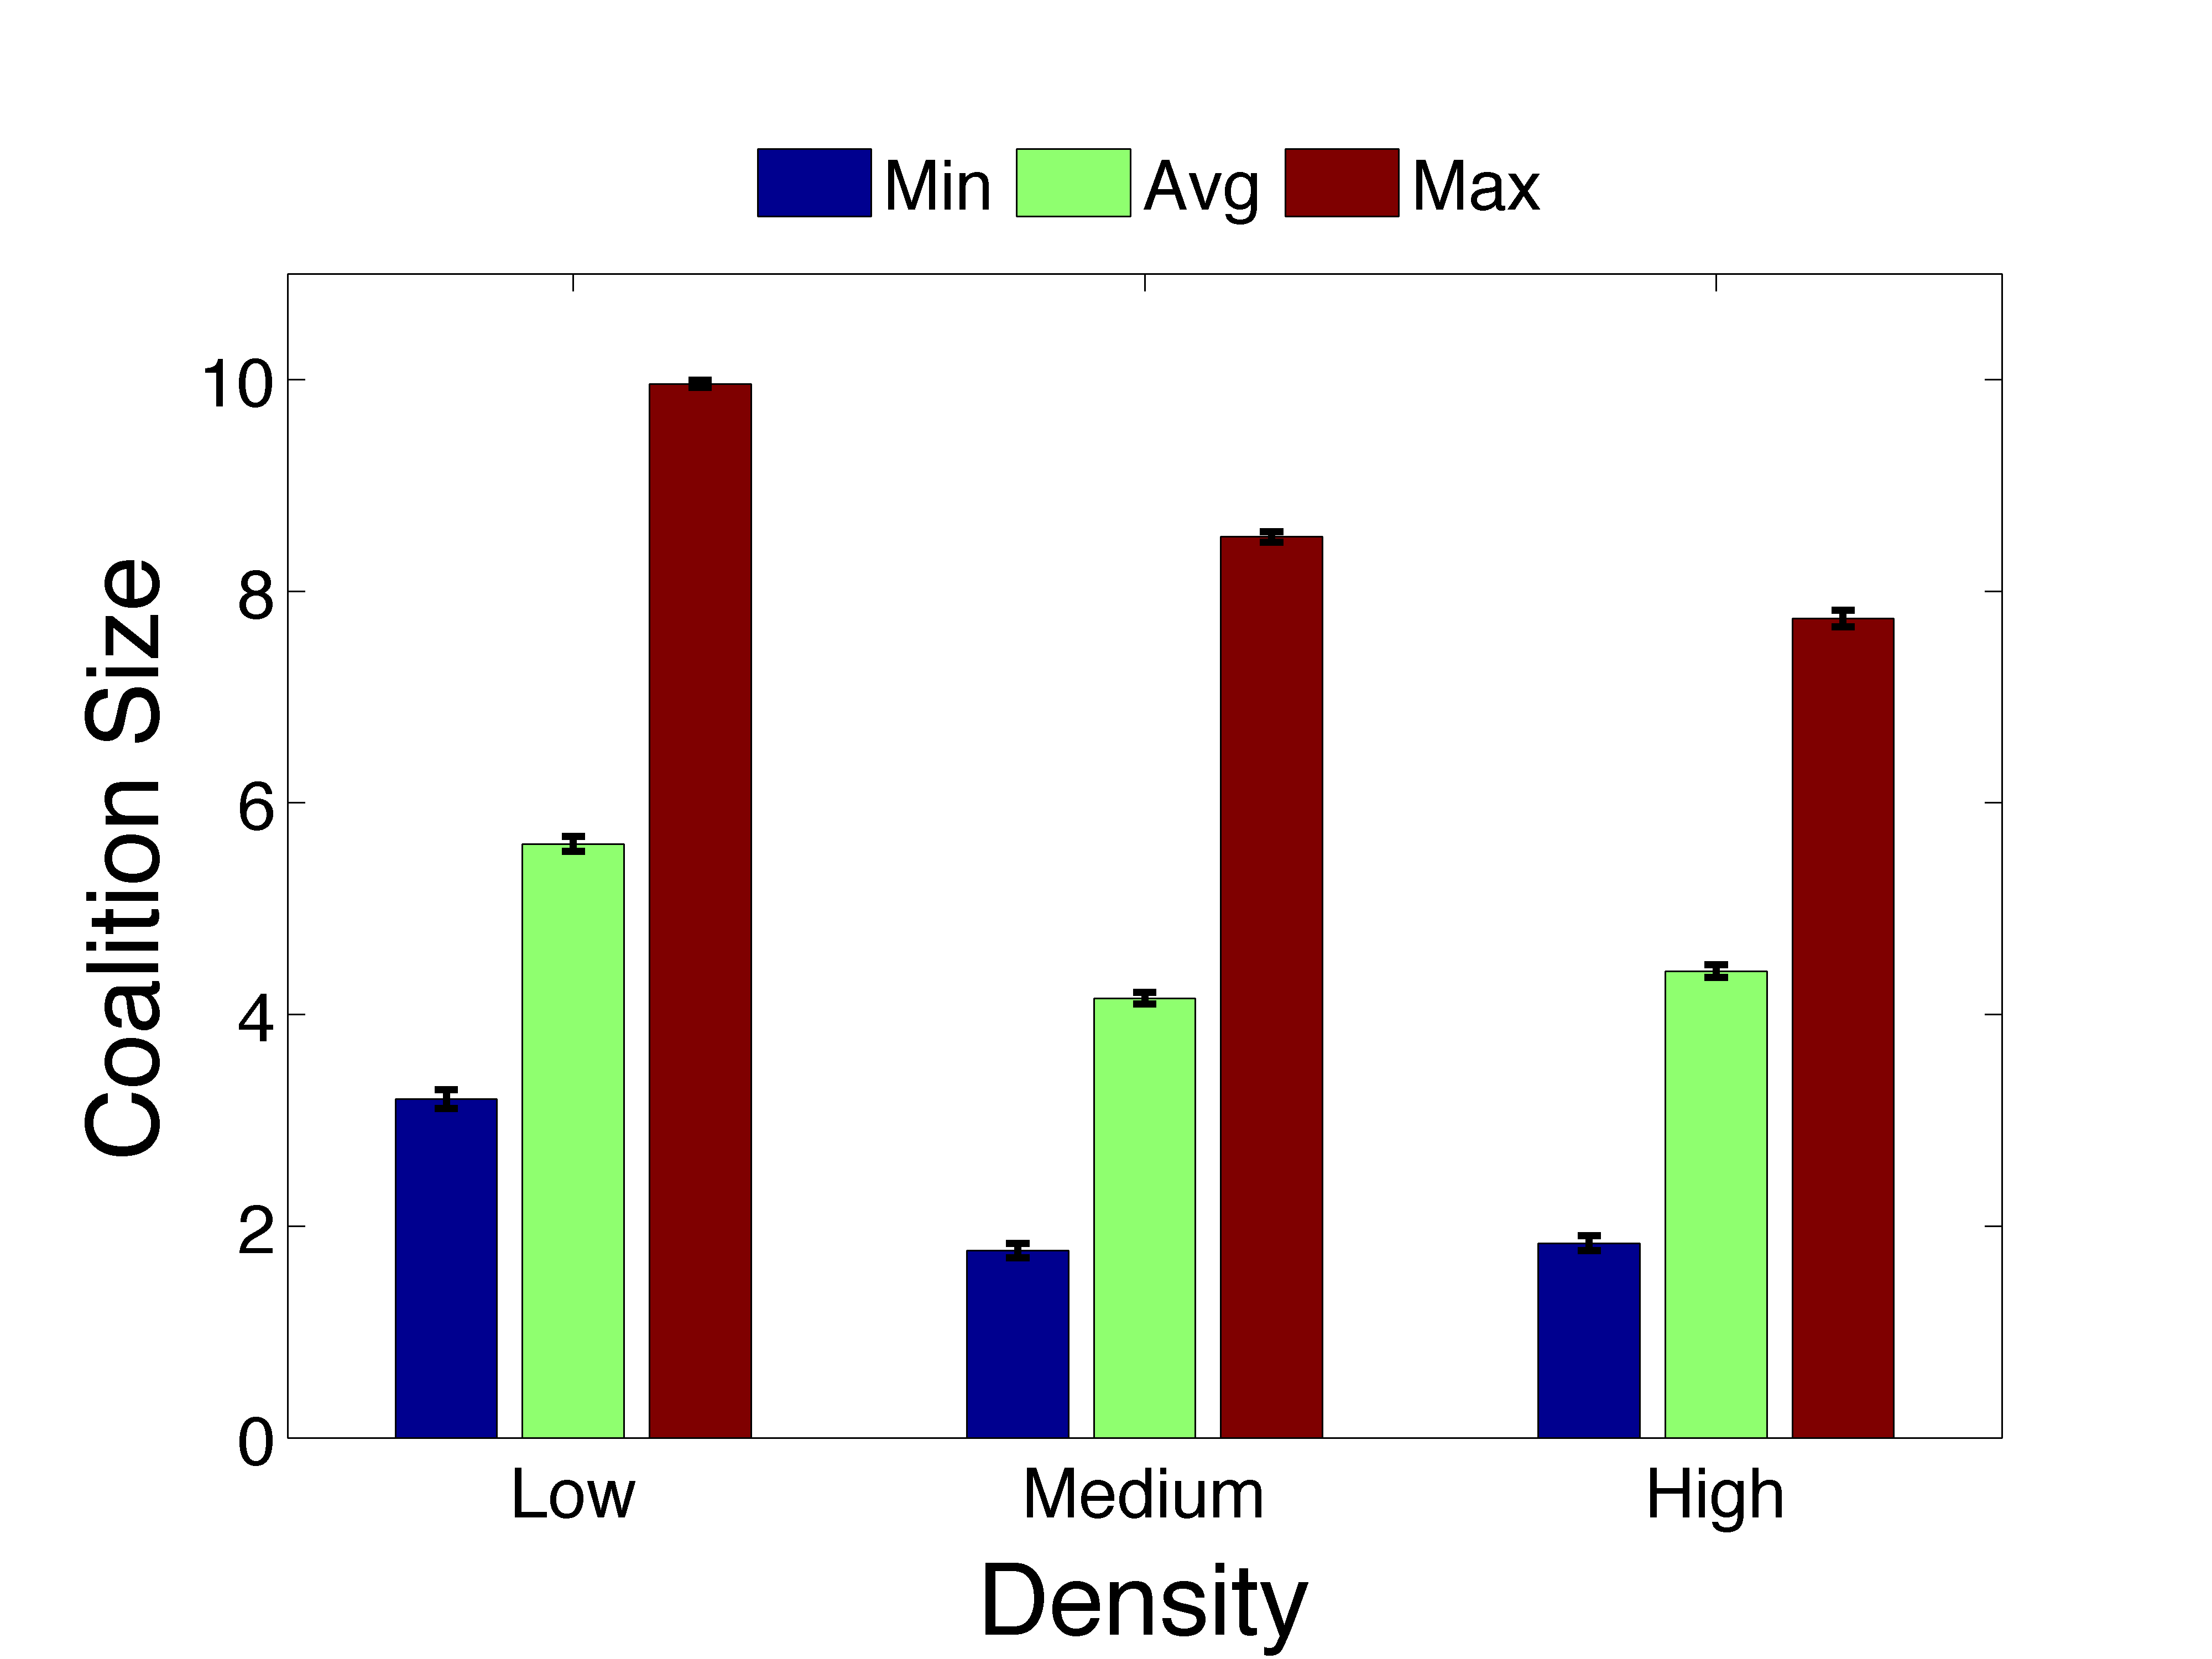
\includegraphics[width=0.3\textwidth,type=png,ext=.png,read=.png]{img/ScaleFree-0.875-Size}
	}  
  \hspace{-0.1in}\subfigure[Small World M2.]{
  	%\label{fig:res_mmuca_quality}
	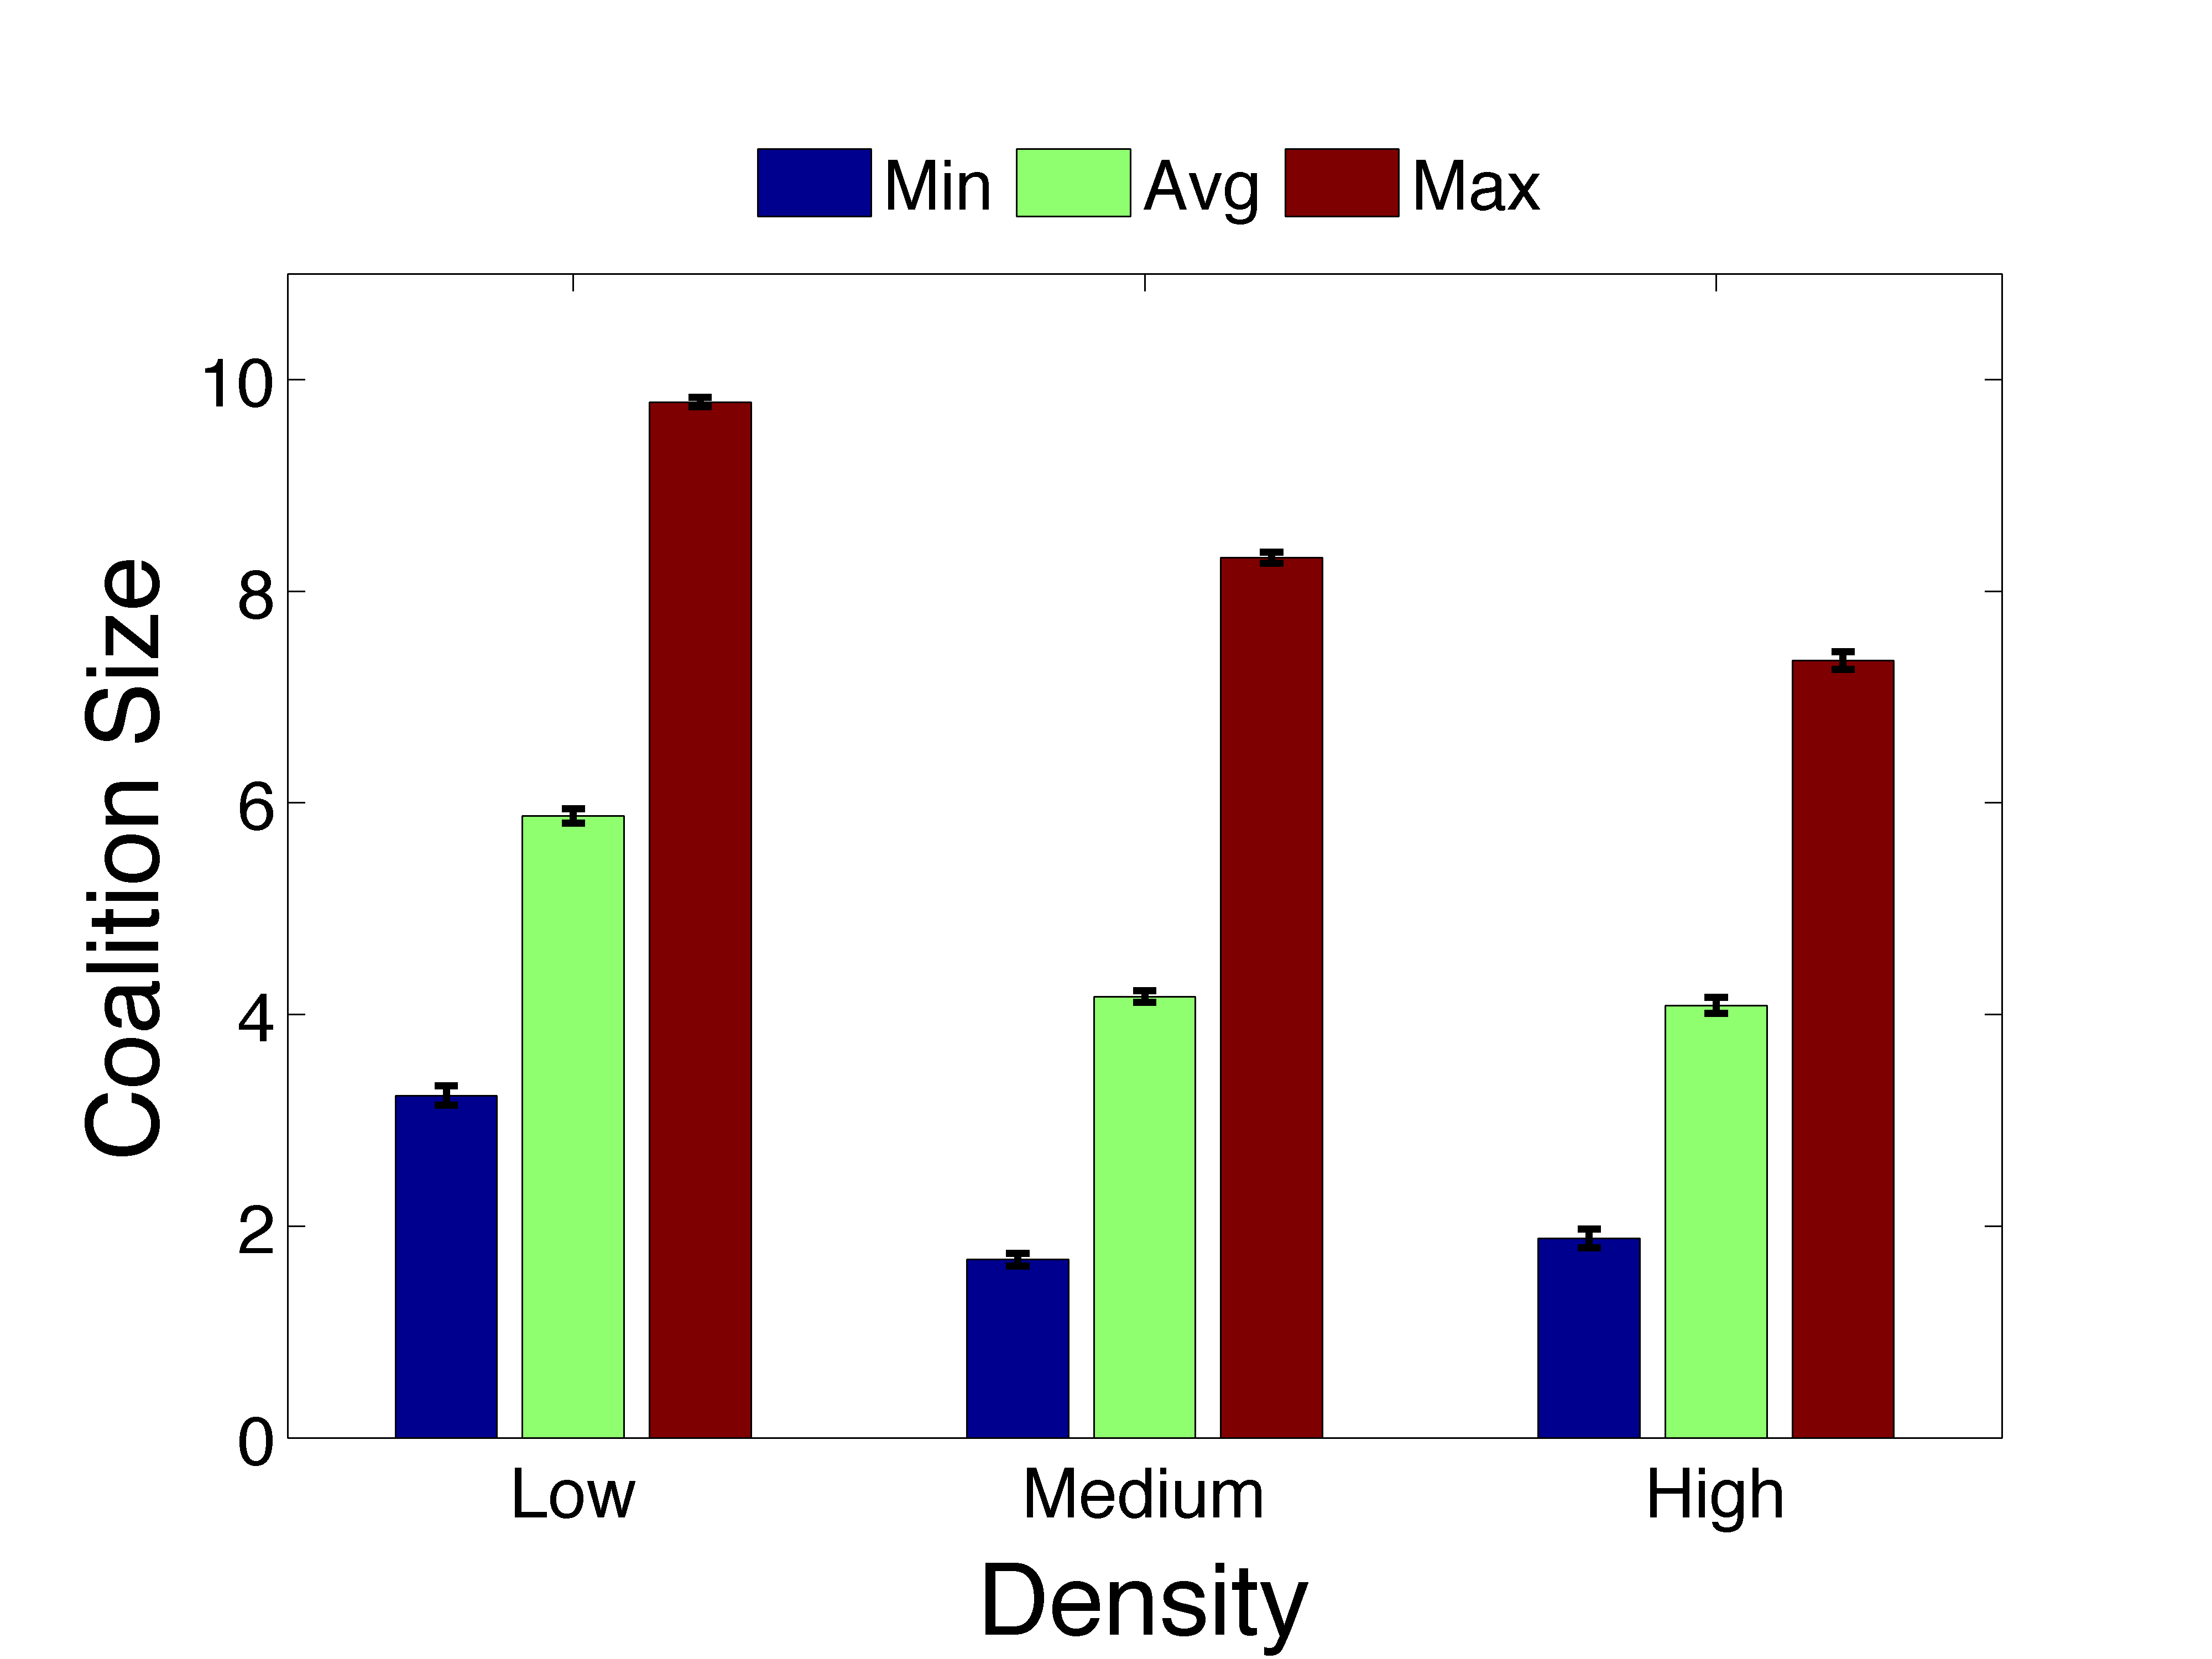
\includegraphics[width=0.3\textwidth,type=png,ext=.png,read=.png]{img/SmallWorld-0.875-Size}
	}  
  \caption{Graphs showing the minimum, average and maximum size of
  coalitions formed on different topologies and densities under market conditions M1 (a)-(c), M2
  (d)-(f). }
  \label{fig:graphs_size}
\end{figure*}     

\begin{table}
\begin{tabular}{ | c | c | c |  c | c |}
\hline
\multirow{2}{*}{\textbf{Topology}} & \multirow{2}{*}{\textbf{Density}}&\multicolumn{3}{c|}{ \textbf{$\%$   Empty Core}}\\
\cline{3-5}
& & M1 & M2 & M3 \\
\hline
\multirow{3}{*}{Random} & Low &  $  8\%$ & $ 0\% $ & $ 0\% $ \\
 & Medium &  $  50\%$ & $ 26\% $ & $ 6\% $ \\
 & High &  $  56\%$ & $ 44\% $ & $ 10\% $ \\
\hline
\multirow{3}{*}{ScaleFree} & Low &  $  0\%$ & $ 0\% $ & $ 0\% $ \\
 & Medium &  $  52\%$ & $ 22\% $ & $ 2\% $ \\
 & High &  $  46\%$ & $ 38\% $ & $ 12\% $ \\
\hline
\multirow{3}{*}{SmallWorld} & Low &  $  8\%$ & $ 6\% $ & $ 2\% $ \\
 & Medium &  $  46\%$ & $ 18\% $ & $ 8\% $ \\
 & High &  $  46\%$ & $ 48\% $ & $ 6\% $ \\
\hline
\end{tabular}
\caption{\label{tab:percentage_core_emptiness} Percentage of instances with empty core under different configurations.}
\end{table}
% \begin{figure*}
%   \centering    
%   \hspace{-0.1in}\subfigure[Random Graphs.]{
%   	%\label{fig:res_walsh_bandwidth}
% 	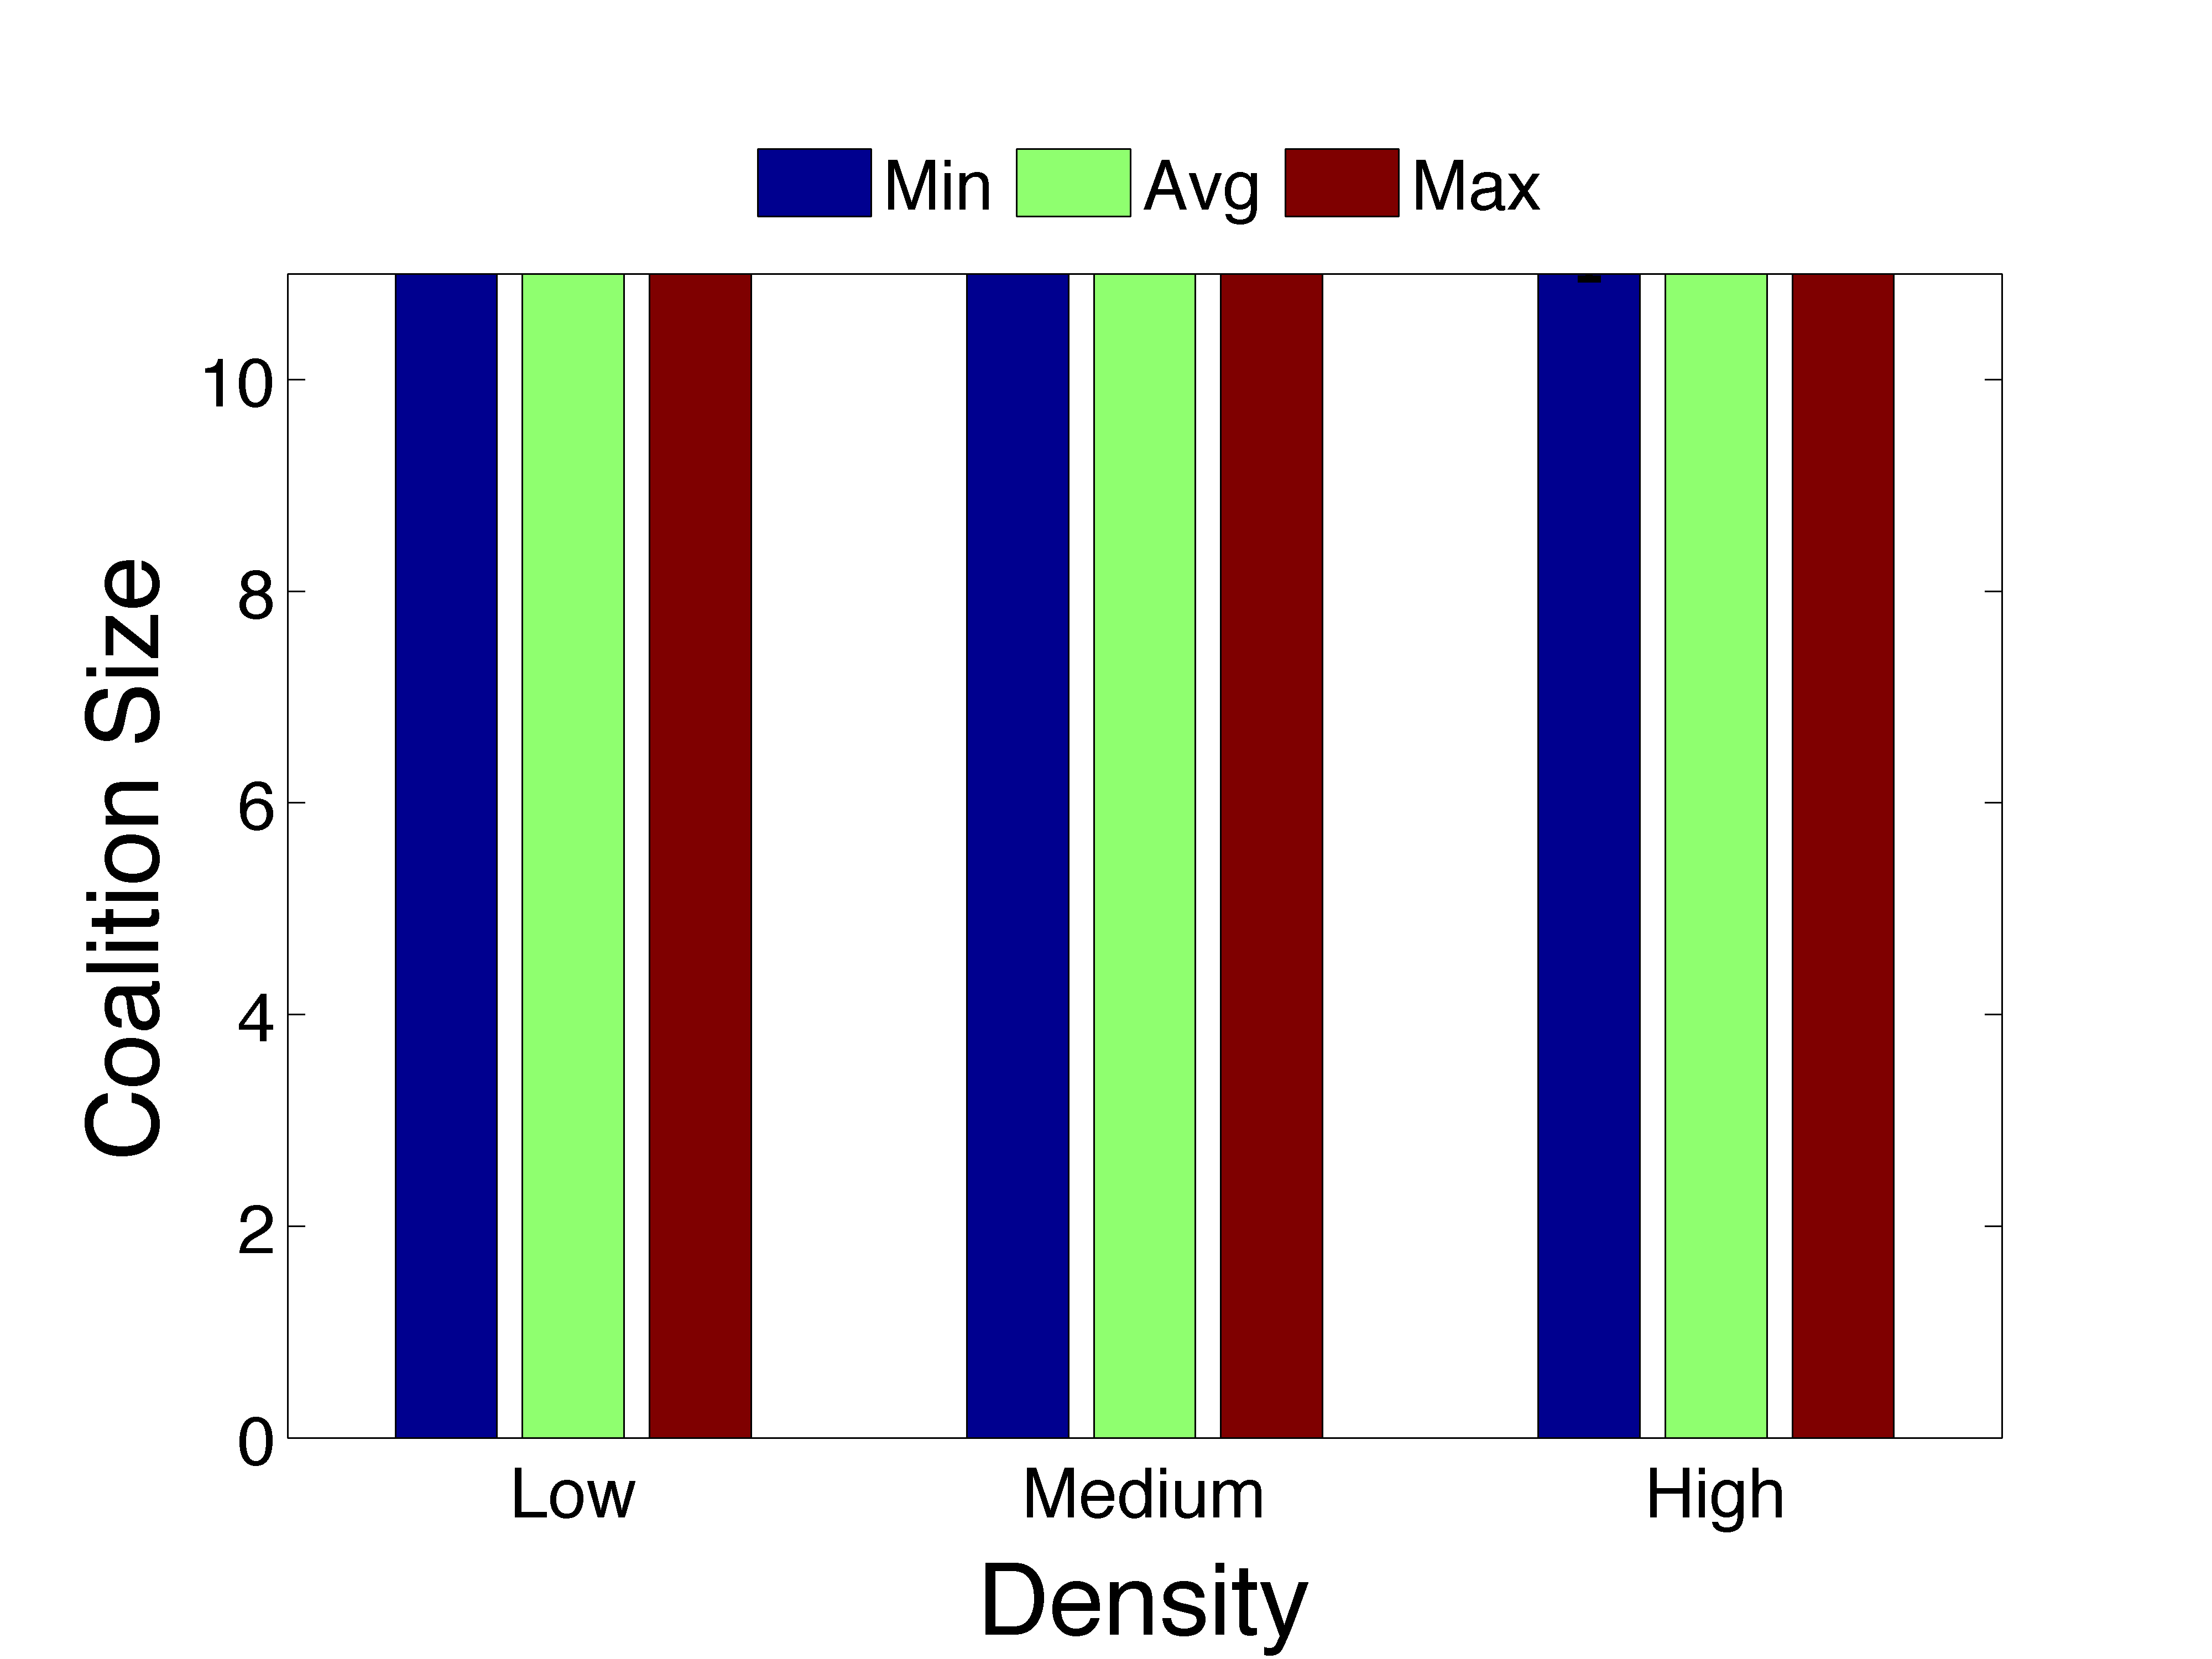
\includegraphics[width=0.33\textwidth,type=png,ext=.png,read=.png]{img/Random-0.500-Size}
% 	}
%   \hspace{-0.1in}\subfigure[Scale Free.]{
%   	%\label{fig:res_mmuca_bandwidth}
% 	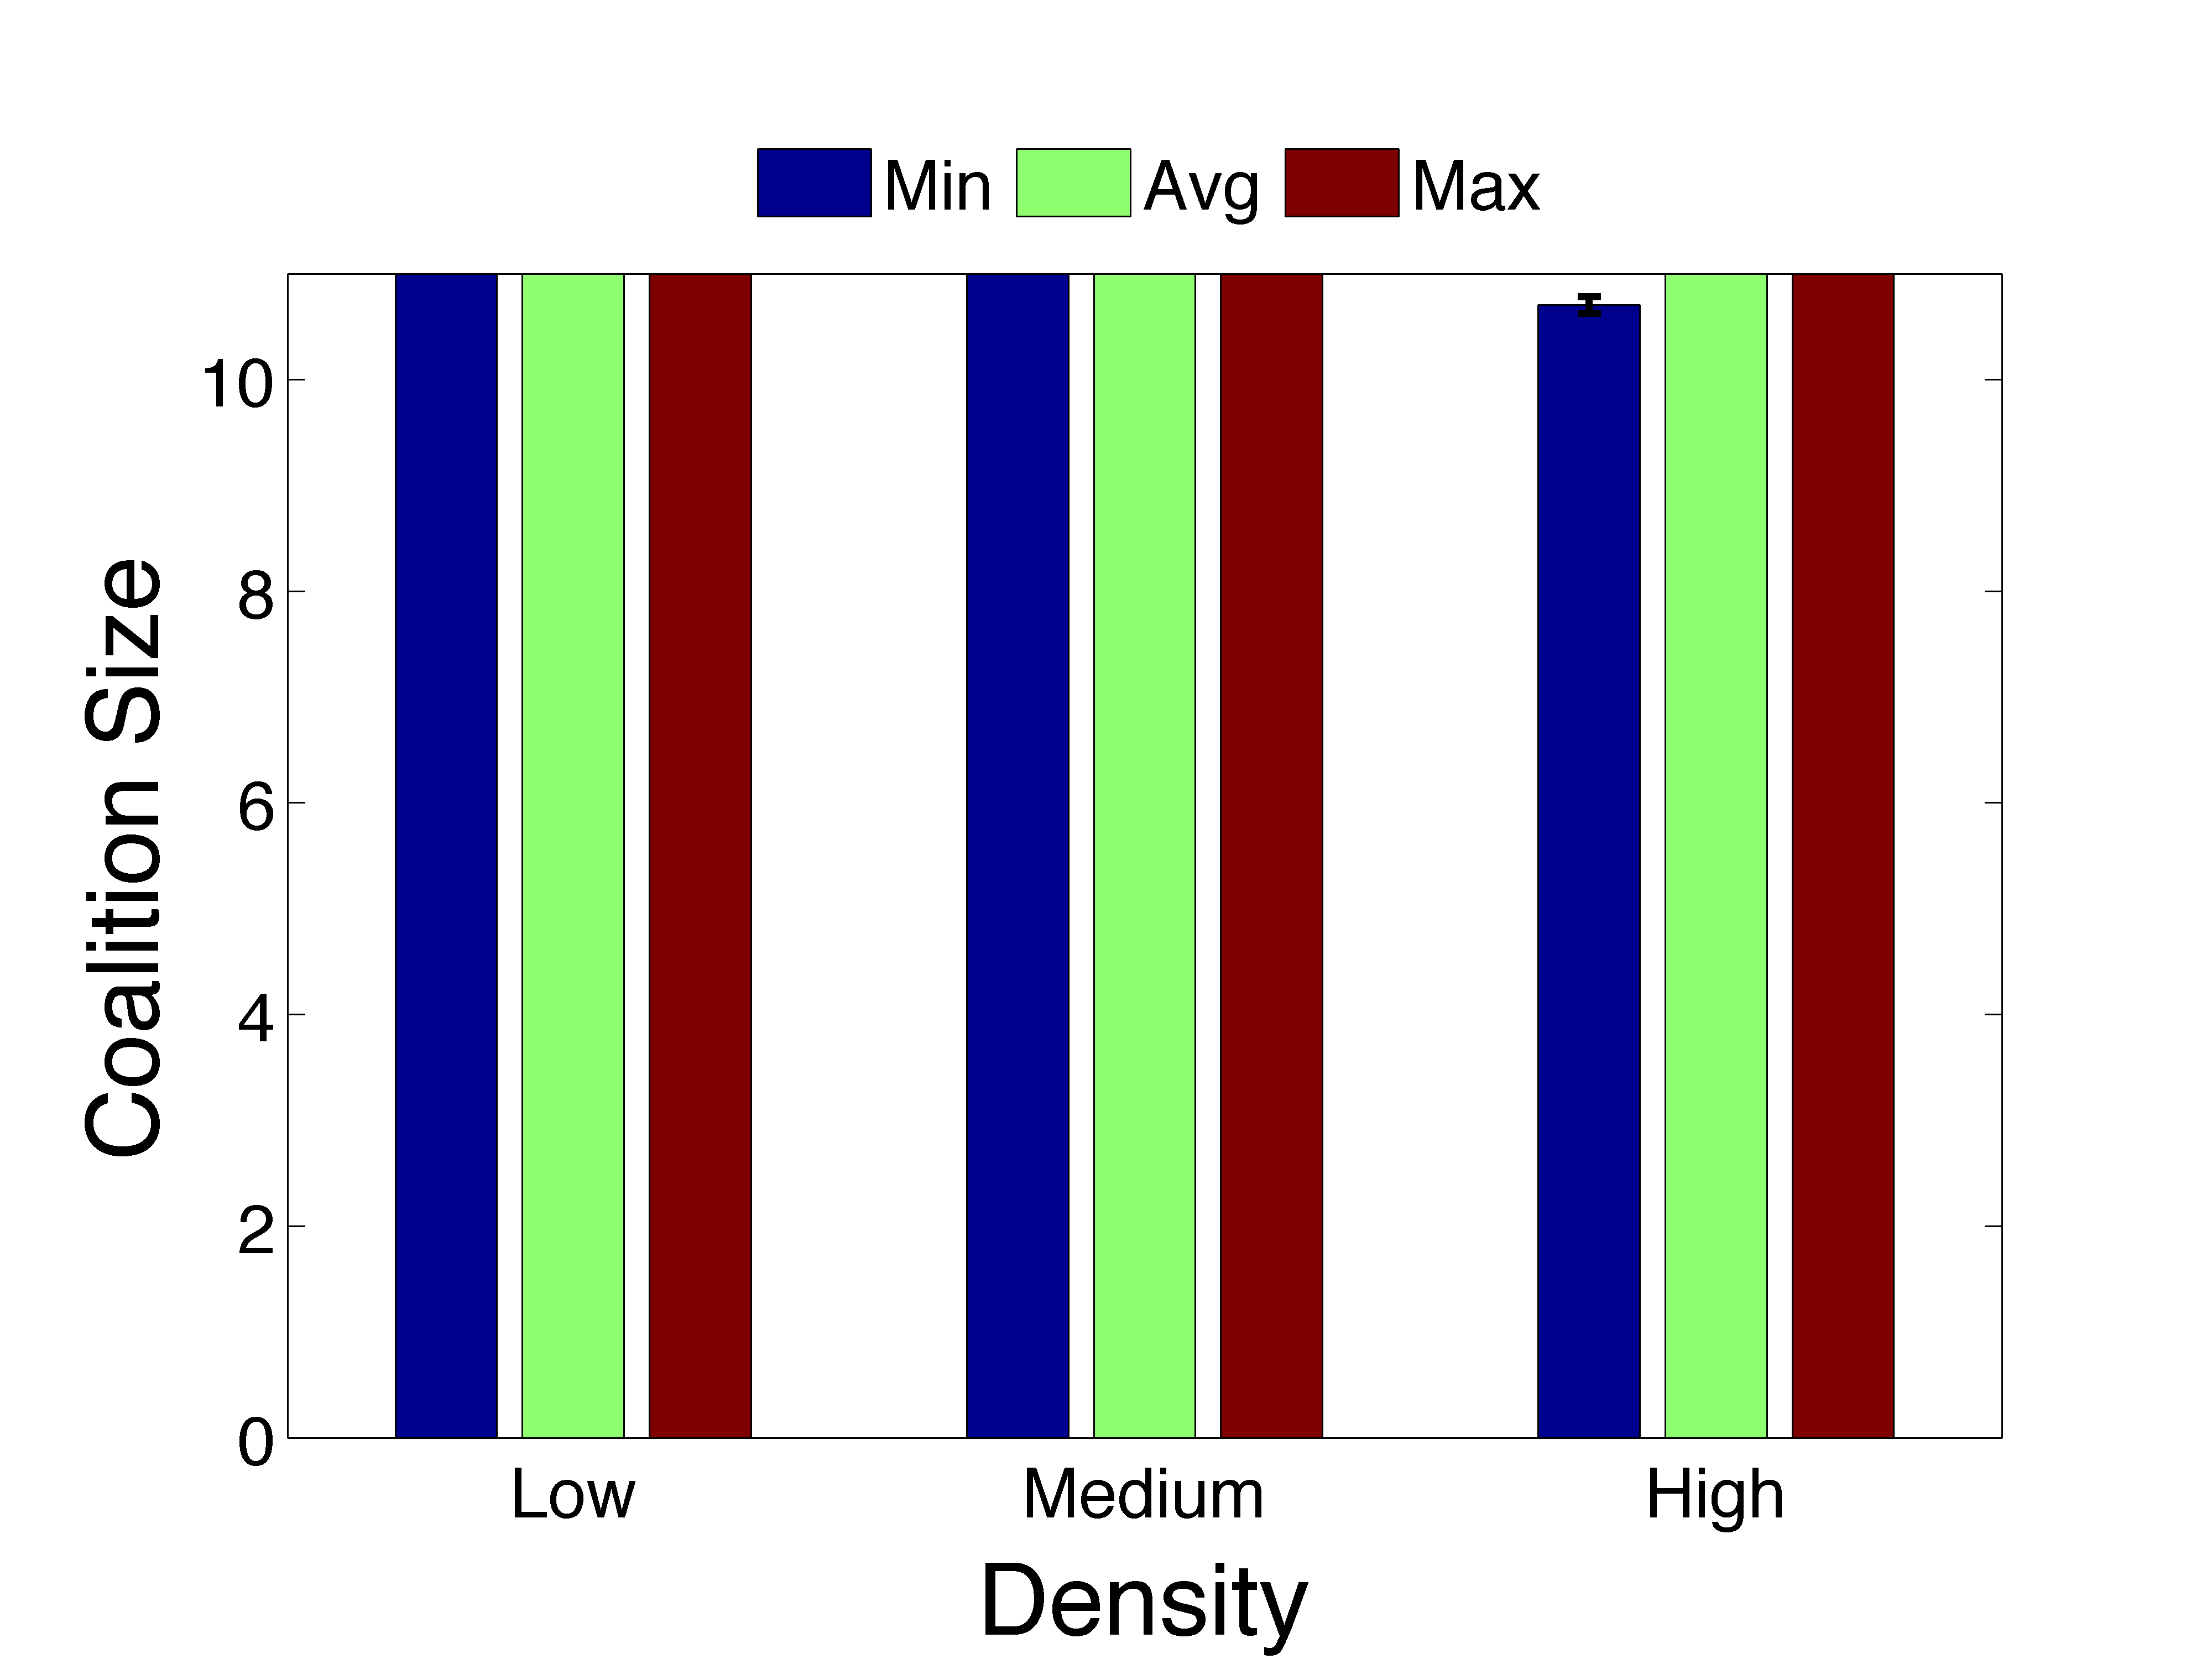
\includegraphics[width=0.33\textwidth,type=png,ext=.png,read=.png]{img/ScaleFree-0.500-Size}
% 	}  
%   \hspace{-0.1in}\subfigure[Small World.]{
%   	%\label{fig:res_mmuca_quality}
% 	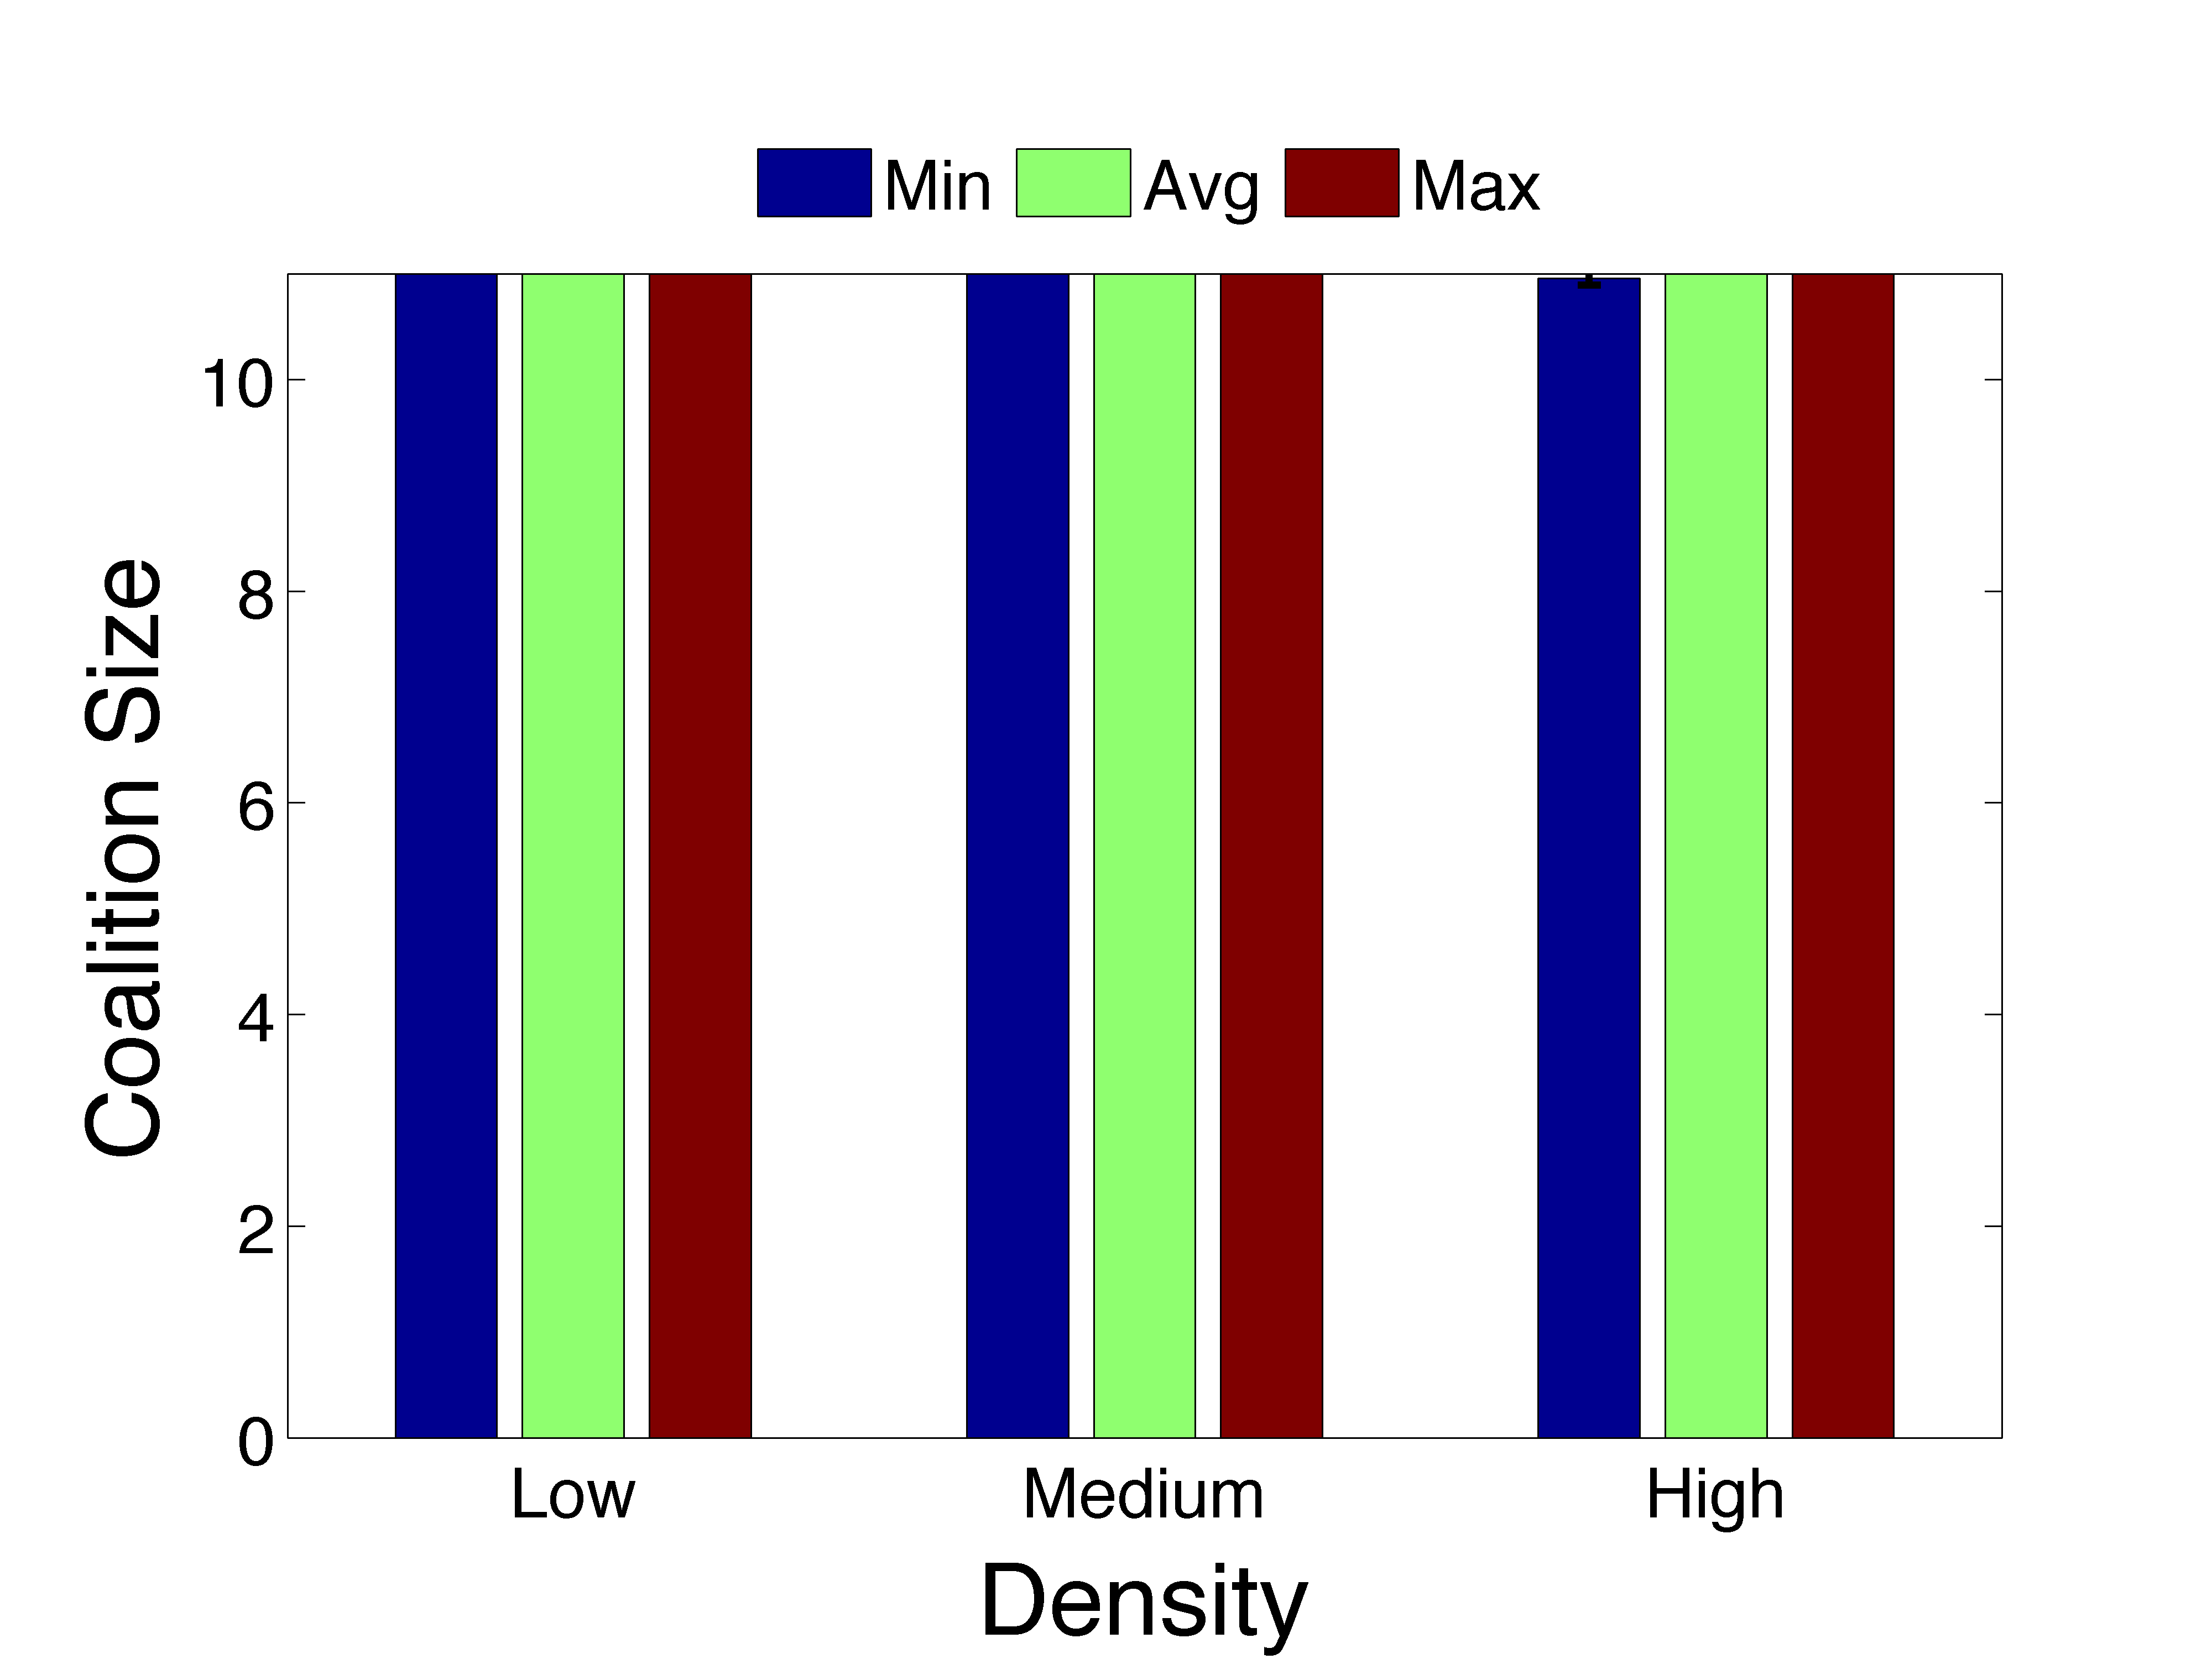
\includegraphics[width=0.33\textwidth,type=png,ext=.png,read=.png]{img/SmallWorld-0.500-Size}
% 	}  
%   \caption{ p=0.500 Graphs showing the minimum, average and maximum size of
%   coalitions formed on different topologies and with different densities. }
%   \label{fig:graphs_size}
% \end{figure*} 








\bibliographystyle{abbrv}

\bibliography{references} 
\end{document}
